\documentclass[a4paper,12pt,openany]{article} 


\usepackage[table]{xcolor}
\usepackage[final]{pdfpages} 

\usepackage{times} 
% this is for the margin for binding in the case of two side printing
\usepackage[hmarginratio=2:2]{geometry}

\usepackage{amsmath, amssymb, latexsym}
\usepackage{amsfonts}
\usepackage{amsthm}
\usepackage{mathtools}
%\usepackage{subfigure}
%\captionsetup[subtable]{position=bottom}
%\usepackage[caption=false,font=footnotesize]{subfig}
\usepackage[utf8]{inputenc}
\usepackage{epsfig}
\usepackage{pdfpages}
\usepackage{booktabs}
\usepackage{float}
\usepackage{wrapfig}
\usepackage{colonequals}
\usepackage{tikz}
\usepackage{xspace}
\usepackage{paralist}
\usetikzlibrary{arrows.meta,decorations.pathmorphing,positioning,fit,trees,shapes,shadows,automata,calc,decorations.markings,patterns} 
\tikzset{>=latex}


\usepackage{protocolj,arydshln}

\usepackage[ruled,vlined,linesnumbered]{algorithm2e}

\setlength{\emergencystretch}{3em} % prevent overfull lines
\providecommand{\tightlist}{%
	\setlength{\itemsep}{0pt}\setlength{\parskip}{0pt}}\setlength{\emergencystretch}{3em} % prevent overfull lines
\providecommand{\tightlist}{%
\setlength{\itemsep}{0pt}\setlength{\parskip}{0pt}}


\usepackage[hyphens]{url}
\usepackage{multirow}
%\usepackage[center, font={small,it}]{caption}
\usepackage[font={small},skip=3pt,belowskip=-7pt]{caption}

\usepackage{subcaption}
\captionsetup{compatibility=false}
\usepackage[bookmarks=true]{hyperref}

\usepackage{array}
\usepackage{rotating}   
\usepackage{makecell}
\usepackage{colortbl}

\usepackage{emptypage}
\usepackage{diagbox}

\usepackage{subfloat}

\usepackage{pifont}

\usepackage{hyperref} % draft for non-clickable links
\usepackage[nameinlink,capitalize]{cleveref}
%\usepackage{graphicx}

\textwidth          150mm
\textheight         225mm
%\oddsidemargin      +6mm
%\evensidemargin     +6mm
%\oddsidemargin      +10mm
%\evensidemargin     +10mm
%\topmargin          -15mm
\topmargin          -5mm

%\usepackage{algorithm}
\usepackage{algpseudocode}

\SetKwInput{KwInput}{Input}                % Set the Input
\SetKwInput{KwOutput}{Output}              % set the Output

\newcommand{\diff}[1]{\textcolor{red}{#1}}

\newcommand{\myparagraph}[1]{\vspace{0.1cm}\noindent{\bf #1.}}

\newcolumntype{P}[1]{>{\centering\arraybackslash}p{#1}}
\newcommand{\Z}{\ensuremath{Z}}
\newcommand{\Zt}{\ensuremath{\Z_t}}
\newcommand{\Zp}{\ensuremath{\Z_p}}
\newcommand{\Zq}{\ensuremath{\Z_q}}
\newcommand{\ZN}{\ensuremath{\Z_N}}
\newcommand{\Zps}{\ensuremath{\Z_p^*}}
\newcommand{\ZNs}{\ensuremath{\Z_N^*}}
\newcommand{\calL}{\ensuremath{\mathcal{L}}}
\newcommand{\calR}{\ensuremath{\mathcal{R}}}
\newcommand{\Prove}{\ensuremath{\mathsf{Prove}}}
\newcommand{\Vrfy}{\ensuremath{\mathsf{Vrfy}}}
\newcommand{\Sim}{\ensuremath{\mathsf{Sim}}}
\newcommand{\Ext}{\ensuremath{\mathsf{Ext}}}
\newcommand{\stmt}{\ensuremath{\mathsf{stmt}}}
\newcommand{\wits}{\ensuremath{\mathsf{wits}}}
\newcommand{\resp}{\ensuremath{\mathsf{resp}}}
\newcommand{\chlg}{\ensuremath{\mathsf{chlg}}}
\newcommand{\mask}{\ensuremath{\mathsf{mask}}}

\newcommand{\Hzk}{\ensuremath{\mathsf{H}_{\mathsf{zk}}}}

\iffalse

	\usepackage[
	automake,
	%acronym, % Create "acronym" glossary, so it can be printed separately
	nogroupskip, % The vertical gaps are caused by a change in letter group. Use nogroupskip to omit them
	nonumberlist, % The number list can be suppressed using the nonumberlist option.
	]{glossaries-extra}
	
	% ############################ Glossaries #####################################
	% Has to be outside preamble to work with latexmkrc
	%\usepackage{makeidx}dbb0a64436904c97afe3e4b28e4f149c4bf93a91
	\usepackage[
	%acronym, % Create "acronym" glossary, so it can be printed separately
	nogroupskip, % The vertical gaps are caused by a change in letter group. Use nogroupskip to omit them
	nonumberlist, % The number list can be suppressed using the nonumberlist option.
	]{glossaries-extra}
	
	\makeindex{}
	\makeglossaries{}
	
	% https://tex.stackexchange.com/questions/437345/acronyms-will-only-display-short-version-in-main-text-even-the-first-time-they
	% First time acronym is used, use long version, afterwards short
	\setabbreviationstyle[acronym]{long-short}
	
	\loadglsentries{glossaries}
	
	% Automatically index the location of entry in the glossary
	% for those entries that are in the "general" category:
	% This indexes every glossary entry by name
	\glssetcategoryattribute{general}{dualindex}{true}
	
	% Emphasize only first use of glossary component
	% https://www.dickimaw-books.com/gallery/index.php?label=mixed-glossary-emph2
	% \renewcommand{\glsxtrregularfont}[1]{\glsxtrifwasfirstuse{\emph{#1}}{#1}}
	\renewcommand{\glsxtrregularfont}[1]{\glsxtrifwasfirstuse{\textit{#1}}{#1}}
	% \renewcommand{\glsxtrabbreviationfont}[1]{\glsxtrifwasfirstuse{\emph{#1}}{#1}}
	%\renewcommand{\glsxtrabbreviationfont}[1]{\glsxtrifwasfirstuse{\textit{#1}}{#1}}
	
	% ########################## End Glossaries ###################################
\fi

%%%% -----------------------------------------------------------------------
%%%% Ryzi Nashovo ekvilibrium
\newcommand{\pnes}{s^{*}}

\newcommand{\gls}[1]{#1}

%%%% -----------------------------------------------------------------------
%%%% Hrac honest a malicious
\newcommand{\phon}{P_{hon}}
\newcommand{\pmal}{P_{grd}}
\newcommand{\halfhalf}{(\frac{1}{2}, \frac{1}{2})}
\newcommand{\bracks}[2]{\left( #1, #2 \right)}

\newtheorem{claim}{Claim}
\newtheorem{definition}{Definition}
\newtheorem{corollary}{Corollary}

\newtheorem{lemma}{Lemma}

\definecolor{ao(english)}{rgb}{0.0, 0.5, 0.0}

\newcommand{\varDash}[1]{{\operatorname{\mathit{#1}}}}

\newtheorem{theorem1}{Security Claim}
\newenvironment{proof1} {\begin{proof}[Justification]} {\end{proof}}


\DeclareUnicodeCharacter{00A0}{ }

\newcommand{\pluseq}{\mathrel{{+}{=}}}
\newcommand{\plusplus}[1]{\mathrel{{#1}{+}{+}}}


%%%% -----------------------------------------------------------------------
%%%% Genericka tabulka zisku v bazove hre
\newcommand{\bazka}[4]{
	\begin{tabular}[t]{c|c|c}
		$\phon$/$\pmal$ & \gls{honest} & \gls{greedy} \\
		\hline
		\gls{honest} & (#1,#1) & (#2,#3) \\
		\hline
		\gls{greedy} & (#3,#2) & (#4,#4) \\
\end{tabular}}


\newtheorem{theorem}{Theorem}
\newtheorem{hypothesis}{Hypothesis}


\newcommand{\goes}[1]{\xrightarrow{#1}}

\newcommand{\reducetool}[0]{\textsc{Reduce}}

\newcommand{\specialcell}[2][c]{%
	\begin{tabular}[#1]{@{}l@{}}#2\end{tabular}}

\usepackage[normalem]{ulem}
\newcommand{\cmark}{\textcolor{black}{\ding{51}}}
\newcommand{\xmark}{\textcolor{black}{\ding{55}}}
\newcommand{\trot}[1]{\multicolumn{1}{l}{\rlap{\rotatebox{25}{#1}~}}}


\algrenewcommand\algorithmiccomment[1]{\hfill \textcolor{gray}{$\triangleright$ \textit{#1}}}


\algnewcommand{\IIf}[1]{\State\algorithmicif\ #1\ \algorithmicthen}
\algnewcommand{\EElse}[1]{\State\algorithmicelse\ #1\ }
\algnewcommand{\EndIIf}{\unskip}
\algrenewcommand\algorithmicindent{1.2em}%

\newcommand*{\dittoclosing}{---''---}


\newcommand{\familymc}{\ensuremath{\mathfrak{D}}}
\newcommand{\init}{\ensuremath{s_0}}
\newcommand{\semantics}[1]{[\![\, #1 \, ]\!]}
%\newcommand{\nils}[1]{\color{blue}Nils: #1\color{black}\xspace}
\newcommand{\pathset}{\mathsf{Paths}}
\newcommand{\paths}[2]{\pathset(#1,\allowbreak\,#2)}
\newcommand{\pathsfin}{\pathset_{\mathit{fin}}}
\newcommand{\pathsinf}{\pathset_{\mathit{inf}}}
\newcommand{\act}{\ensuremath{a}}
\newcommand{\Act}{\ensuremath{\mathit{Act}}}
\newcommand{\last}[1]{\mathrm{last}(#1)}
\DeclareMathOperator{\supp}{supp}
\DeclareMathOperator{\successors}{succ}
\newcommand{\Distr}{\mathit{Distr}}
\newcommand{\subDistr}{\mathit{subDistr}}
\newcommand{\distDom}{X}
%\newcommand{\distDomFin}{\DistDom=\{x_1,\, \ldots,\, x_n}
\newcommand{\distFunc}{\mu}
\newcommand{\distDomElem}{x}
\newcommand{\true}{\texttt{true}\xspace}
\newcommand{\false}{\texttt{false}\xspace}
\newcommand{\probOneG}{\mathit{p1G}}
\newcommand{\probPosG}{\mathit{pPG}}
\newcommand{\quotientstates}{\ensuremath{S^\mathfrak{D}_\sim}}
\newcommand{\abs}{\text{abs}}
\newcommand{\queue}{\ensuremath{Q}}
\newcommand{\submc}[2]{\ensuremath{{#1}\!\downarrow\!{#2}}}


\newcommand{\dtmc}{\ensuremath{D}}
\newcommand{\mdp}{\ensuremath{M}}
\newcommand{\probdtmc}{\ensuremath{P}}
\newcommand{\probfam}{\ensuremath{\mathfrak{P}}}
\newcommand{\sched}{\ensuremath{\sigma}}
\newcommand{\induced}[2]{\ensuremath{{#1}_{#2}}}
\newcommand{\Succ}{\ensuremath{\mathsf{Succ}}}

\newcommand{\Option}{\mathsf{Option}}
\newcommand{\Sketch}{\mathfrak{S}_H}
\newcommand{\ProgHoles}{\mathfrak{P}_H}
\newcommand{\program}[2]{\mathfrak{#1}_{#2}}
\newcommand{\SketchConstraints}{\ensuremath{\Gamma}}
\newcommand{\OptionPrices}{\ensuremath{\mathsf{cost}}}

\newcommand{\Assignments}[1]{\mathcal{A}_{#1}}
\newcommand{\var}{\xi}
\newcommand{\dom}{\textsl{dom}}

\newcommand{\actionof}[1]{\mathrm{act}(#1)}
\newcommand{\varHigh}{\xi}
\newcommand{\Vars}{\mathrm{Var}}
\newcommand{\modules}{\mathcal{M}}
\newcommand{\enabled}{\mathsf{enabled}}
\newcommand{\Prob}{\mathsf{Prob}}
\newcommand{\fixdeadlock}{\mathsf{fixdl}}

\newcommand{\crn}{\mathcal{N}}
\newcommand{\concMC}{\gamma(\crn)}
\newcommand{\absMC}{\alpha(\crn)}
\newcommand{\absIMC}{\alpha(\crn)}

\newcommand{\pspace}{\mathcal{P}}
\newcommand{\tspace}{\mathcal{T}}
\newcommand{\uspace}{\mathcal{U}}
\newcommand{\fspace}{\mathcal{F}}
\newcommand{\rspace}{\mathcal{R}}

\newcommand{\model}{\ensuremath{\mathcal{C}}}

\newcommand{\distr}{\pi}
\newcommand{\tmat}{\mathbf{R}}
\newcommand{\states}{S}
\newcommand{\state}{s}
\newcommand{\pmat}{\mathbf{P}}
\newcommand{\propQM}{=?}

\newcommand{\propTrue}{\mbox{\tt true}}
\newcommand{\propFalse}{\mbox{\tt false}}

\newcommand{\pathF}{\ensuremath{\phi}}
\newcommand{\stateF}{\ensuremath{\Phi}}


\newcommand{\propP}{\mbox{P}}
\newcommand{\propU}{\mbox{U}}
\newcommand{\propG}{\mbox{G}}
\newcommand{\propF}{\mbox{F}}
\newcommand{\propC}{\mbox{C}}
\newcommand{\propI}{\mbox{I}}
\newcommand{\propR}{\mbox{R}}
\newcommand{\propX}{\mbox{X}}

\newcommand{\satfun}{\ensuremath{\Lambda}}

\newcommand{\CTMC}{\ensuremath{\mathcal{C}=(S,\pi_0, \mathbf{R}, L)}}
\newcommand{\pp}{\ensuremath{\gamma}}
\newcommand{\ddistr}{\tau}

\newcommand{\Path}{\mbox{Path}}

\newcommand{\toolname}{PRISM-PSY}


\usepackage{listings}


% tikzstyles
\definecolor{prismgreen}{HTML}{009900}
\definecolor{prismred}{HTML}{cc0000}
\definecolor{prismblue}{HTML}{0000cc}



% PRISM syntax highlighting
\lstdefinelanguage{Prism}{
        basicstyle=\color{prismred}\scriptsize\ttfamily,
        literate=*	{0}{{\textcolor{prismblue}{0}}}{1}
			{1}{{\textcolor{prismblue}{1}}}{1}
			{2}{{\textcolor{prismblue}{2}}}{1}
			{3}{{\textcolor{prismblue}{3}}}{1}
			{4}{{\textcolor{prismblue}{4}}}{1}
			{5}{{\textcolor{prismblue}{5}}}{1}
			{6}{{\textcolor{prismblue}{6}}}{1}
			{7}{{\textcolor{prismblue}{7}}}{1}
			{8}{{\textcolor{prismblue}{8}}}{1}
			{9}{{\textcolor{prismblue}{9}}}{1}
			{.0}{{\textcolor{prismblue}{.0}}}{2}
			{.1}{{\textcolor{prismblue}{.1}}}{2}
			{.2}{{\textcolor{prismblue}{.2}}}{2}
			{.3}{{\textcolor{prismblue}{.3}}}{2}
			{.4}{{\textcolor{prismblue}{.4}}}{2}
			{.5}{{\textcolor{prismblue}{.5}}}{2}
			{.6}{{\textcolor{prismblue}{.6}}}{2}
			{.7}{{\textcolor{prismblue}{.7}}}{2}
			{.8}{{\textcolor{prismblue}{.8}}}{2}
			{.9}{{\textcolor{prismblue}{.9}}}{2}
			{[}{{\textcolor{black}{[}}}{1}
			{]}{{\textcolor{black}{]}}}{1}
			{+}{{\textcolor{black}{+}}}{1}
			{-}{{\textcolor{black}{-}}}{1}
			{=}{{\textcolor{black}{=}}}{1}
			{<}{{\textcolor{black}{<}}}{1}
			{>}{{\textcolor{black}{>}}}{1}
			{\&}{{\textcolor{black}{\&}}}{1}
			{|}{{\textcolor{black}{|}}}{1}
			{:}{{\textcolor{black}{:}}}{1}
			{;}{{\textcolor{black}{;}}}{1}
			{(}{{\textcolor{black}{(}}}{1}
			{)}{{\textcolor{black}{)}}}{1}
			{..}{{\textcolor{black}{..}}}{2},
        keywords= {bool,ceil,const,ctmc,double,dtmc,endinit,endmodule,endrewards, endsystem,F,false,floor,formula,G,global,I,init,int,label,max,mdp,min,module,nondeterministic,P,Pmin,Pmax,prob,probabilistic,rate,rewards,Rmin,Rmax,S,stochastic,system,true,U, option, either, assignment, relation, operation, hole, variable},
        keywordstyle={\bfseries\color{black}},
        numberstyle=\footnotesize\color{black},
        comment=[l] {//}, morecomment=[s]{/*}{*/},
        commentstyle= \color{prismgreen},
        tabsize=4,
        captionpos=b,
        escapechar=^,
        moredelim=[is][\color{orange}]{@}{@},
}


\usepackage{nicefrac}


\newcommand{\ih}[1]{\textcolor{blue}{\footnotesize [IH: #1]}}

\hyphenation{block-chain block-chains Smart-OTPs free-ness Strong-Chain gree-dy}

\newcommand{\name}{CHANGE-ME\xspace}%


\begin{document} 

\thispagestyle{empty}


\includegraphics[width=150mm]{figs/FIT_color_CMYK_EN.pdf}
{\fontfamily{ptm}\selectfont

%{\huge Brno University of Technology}         \\[2mm]
%{\LARGE Faculty of Information Technology}    \\[50mm]

\vspace{5cm}


\begin{center}
  {\large Lecture Notes for the Course}      \\[10mm]
  {\LARGE \bf Blockchains and Decentralized Applications}    
  
\end{center}                                            
 
 \vfill
                 
\large doc. Ing. Ivan Homoliak  Ph.D.                                   
  \hfill  Brno 2025                                  


}

\thispagestyle{empty}

\eject

\thispagestyle{empty}

\ \\



\pagenumbering{roman}

%------------------------------------------------------------------------------
\section*{Abstract}
%------------------------------------------------------------------------------
The course Blockchain and Decentralized Applications (BDA) aims to acquaint students with the principles and protocols in fully decentralized (P2P) network communication. While aspects of client-server communication are important, the less traditional but emerging peer-to-peer blockchain scheme and its integration into the Internet is an alternative that allows us to achieve unique features in terms of availability, transparency, and trust. This course focuses on the technical aspects of blockchain systems, smart contracts, and decentralized applications. Students will learn how these systems are built, how to communicate with them, and how to design \& create secure decentralized applications. Students will also exercise the acquired knowledge in practice through a semestral assignment.
Students will learn advanced theoretical and practical knowledge in the field of decentralized computing platforms, their types, consensual protocols, and problems associated with them. Further, students will learn knowledge of terminology, unique properties of blockchain, knowledge of advanced integrity-preserving data structures and algorithms used in blockchains and smart contract platforms. the next goal is to present practical use cases and their potential vulnerabilities. The course also deals with the problem of scalability and anonymity and variants of their solution. In sum, students should obtain the ability to design, deploy, and manage custom decentralized applications and solutions.
%------------------------------------------------------------------------------
\section*{Keywords}
%------------------------------------------------------------------------------
Decentralized platforms, blockchains, integrity-preserving data structures, smart contracts, decentralized applications, DAPPs, consensus protocols, security threats, scalability, anonymity, and privacy.
%Security, privacy, blockchains, distributed ledgers, threat modeling, standardization, decentralized applications, consensus protocols, proof-of-work, selfish mining attacks, undercutting attacks, incentive attacks, DAG-based blockchains, cryptocurrency wallets, two-factor authentication, 2FA, electronic voting, e-voting, public bulletin board, secure logging, data provenance, interoperability, Central Bank Digital Currency, CBDC, Trusted Execution Environment, TEE, cross-chain protocol.


\clearpage
%
%------------------------------------------------------------------------------
\section*{Acknowledgment}
%------------------------------------------------------------------------------
First, I would like to thank my supervisor and colleague from SUTD -- Pawel Szalachowski -- for collaborating and igniting many interesting research ideas as well as explaining to me that ideas are important but cheap in contrast to realization. 
Second, I would like to thank all my co-authors, especially Sarad Venugopalan, Pieter Hartel, Daniel Reijsbergen, Federico~Matteo Ben{\v{c}}i{\'c}, Fran Casino, and Martin Hrub{\'y}. 
%
Third, I would like to thank Tomas Vojnar, Pavel Zemcik, Pavel Smrz, and Ales Smrcka for their support in funding my research at FIT BUT.
Next, I would like to thank all Ph.D./MSc/BSc students I have had the chance to work with, especially Martin Peresini, Ivana Stan{\v{c}}{\'\i}kov{\'a}, and Dominik Breitenbacher / Tomas Hladky, Jakub Handzus, Jakub Kubik, and Martin Ersek / and Rastislav Budinsk{\'y}. 
%
Also, I would like to thank Milan Ceska (and Tomas Vojnar) for inspiring me in the habilitation process and helping me to maximize cross-domain transfer learning in this process.  
Finally, I would like to thank around 20\% of anonymous reviewers (mostly from security venues) for providing useful and constructive feedback. % or reasonable arguments.




%First, I would like to thank my advisers and mentors: Lubo\v{s} Brim for starting my research and academic career, Marta Kwiatkowska for providing me the world-leading expertise in the area of probabilistic verification and Tom\'{a}\v{s} Vojnar for helping me to establish my own research group.
%Second, I would like to thank all my co-authors, especially David \v{S}afr\'{a}nek, Nicola Paoletti, Alessandro Abate, Radu Calinescu, Joost-Pieter Katoen, Ond\v{r}ej Leng\'{a}l, Luk\'{a}\v{s} Hol\'{i}k, and Jan K\v{r}et\'{i}nsk\'{y}. Third, I would like to thank all Ph.D. students I had the chance to work with especially Sven Dra\v{z}an, Luca Laurenti, Simos Gerasimou, Ji\v{r}\'{i} Maty\'{a}\v{s}, Vojta Havlena and Sebastian Junges. Last but not least, I would like to thank Gabina for supporting me during my entire research career and my parents for inspiring me to take this career. 


\vfill \emph{Over the time, I have been supported by number of projects, in particular, by EU ECSEL projects, EU HORIZON EUROPE projects, National Research Foundation -- Prime Minister's Office in Singapore, Technology Agency of the Czech Republic, and the Czech IT4Innovations Centre of Excellence project.
%Czech Science Foundation project
}


\newtheorem{mydef}{Definition}
\newtheorem{example}{Example}
\newtheorem{myproof}{Proof}
\newtheorem{myproposition}{Proposition}
\newtheorem{mytheorem}{Theorem}
\newtheorem{myexample}{Example}
\newtheorem{myproblem}{Problem}
\newtheorem{mycorollary}{Corollary}
\newtheorem{mymethod}{Approach}
\newtheorem{remark}{Remark}


\renewcommand{\tableautorefname}{Table}
\renewcommand{\algorithmautorefname}{Algorithm}
\renewcommand{\figureautorefname}{Figure}
\renewcommand{\equationautorefname}{Equation}
\renewcommand{\sectionautorefname}{Appendix}

\renewcommand{\chapterautorefname}{Chapter}
\renewcommand{\sectionautorefname}{Section}
\renewcommand{\subsectionautorefname}{Section}
\renewcommand{\subsubsectionautorefname}{Section}
\renewcommand{\paragraphautorefname}{ Section}
\renewcommand{\tablename}{Table}
\renewcommand{\figurename}{Figure}
%\newcommand{\subfigureautorefname}{\figureautorefname}

\newcommand{\mysubsubsection}[1]{\smallskip\subsubsection{#1}}


\tableofcontents

\newcommand{\squishlist}{
   \begin{list}{$\bullet$}
    { \setlength{\itemsep}{5pt}    \setlength{\parsep}{0pt}
      \setlength{\topsep}{5pt}     \setlength{\partopsep}{0pt}
      \setlength{\leftmargin}{1.35em} \setlength{\labelwidth}{1em}
      \setlength{\labelsep}{0.5em} } }

\newcommand{\squishend}{
    \end{list}  }


\clearpage
\pagenumbering{arabic}



%\part{COMMENTARY}
%\part{COMMENTED RESEARCH}

\section{Introduction and Required Cryptographic Constructs}\label{sec:intro}
%\subsection{Introduction}\label{introduction}

This section serves as a comprehensive introduction to the course of
Blockchains and Decentralized Applications (BDA). It begins by outlining
the course's core objectives, which are designed to provide both
theoretical knowledge and practical skills in this rapidly evolving
domain. 
%The section details the course structure, including the lecture
%schedule, project requirements, and examination policies, to provide a
%clear roadmap for the semester. A significant portion of this
%introduction is dedicated to presenting the instructors, a team of
%seasoned academics and industry practitioners, whose collective
%expertise spans the critical areas of blockchain technology, from
%consensus protocols and system security to zero-knowledge cryptography
%and forensic analysis.

The primary objective of this section is to establish a solid foundation
for the topics that will be explored in subsequent sections. To this
end, it delves into the fundamental cryptographic constructs that are
indispensable for understanding the inner workings of blockchain
systems. These include a detailed examination of cryptographic hash
functions, which ensure data integrity; hash chains, a simple yet
powerful tool for creating cryptographically connected sequences; Merkle trees, an
efficient data structure for verifying the contents of large data sets;
and digital signatures, the mechanism that provides authenticity and
non-repudiation in a decentralized environment. A thorough understanding
of these cryptographic primitives is paramount, as they form the bedrock
upon which the security, immutability, and trustworthiness of
blockchains are built.

\subsection{Learning Objectives of the Course}\label{learning-objectives}

\begin{itemize}
	\tightlist
	\item
	Gain theoretical and practical knowledge in the field of BDA, their
	types, consensual protocols, and pros/cons.
	\item
	Understand the terminology, unique properties of blockchain,
	integrity-preserving data structures, and algorithms.
	\item
	Learn about practical use cases and their potential vulnerabilities.
	\item
	Understand the scalability/throughput problems and their solutions.
	\item
	Grasp the privacy aspects and variants of their solution.
	\item
	Develop the ability to design, implement, and deploy custom DAPPs and
	blockchains.
\end{itemize}

\begin{center}\rule{0.5\linewidth}{0.5pt}\end{center}

\subsection{Course Overview}\label{section-1-course-overview}

\subsubsection{About the Instructors}\label{about-the-instructors}

The course is led by a team of experienced researchers and practitioners
in the field of blockchain technology, each bringing a unique set of
skills and experiences to the curriculum.
The following listings contains current and former course instructors who helped in running this course.
\begin{itemize}
	\item
	\textbf{doc. Ing. Ivan Homoliak, Ph.D.} (Guarantor): Dr.~Homoliak is
	an associate professor at the Faculty of Information Technology, Brno
	University of Technology (FIT@BUT). His academic journey includes a
	Ph.D.~from FIT@BUT in 2016, followed by a postdoctoral fellowship at
	the Singapore University of Technology and Design (SUTD), where his
	research was centered on blockchains and cybersecurity. His
	habilitation, titled ``Towards Secure Consensus Protocols and
	Decentralized Applications in Blockchains,'' \ih{cite} underscores his deep
	expertise in the field. Dr.~Homoliak's research interests are
	extensive and include electronic voting in blockchains~\cite{homoliak2023bbb,venugopalan2023always,stanvcikova2022sbvote,homoliak2025votemate}, the security
	and scalability of consensus protocols~\cite{perevsini2023incentive,perevsini2021dag,perevsini2023dag,budinsky2023fee}, the intersection of Trusted
	Execution Environments (TEE) with blockchain technology~\cite{homoliak2020aquareum}, Central Bank
	Digital Currencies (CBDC)~\cite{homoliak2023cbdc}, and the application of zero-knowledge
	cryptography~\cite{perevsini2025featherwallet} \ih{todo}.
	\item
	\textbf{Ing. Vladimír Veselý, Ph.D.} (Guarantor Deputy): Dr.~Veselý's
	engagement with cryptocurrencies dates back to 2011, when he began
	mining Bitcoin. His practical experience is complemented by a
	Ph.D.~from FIT@BUT. He serves as a consultant for law enforcement
	agencies on cryptocurrency-related crimes, a role that leverages his
	deep understanding of forensic analysis and the tracking of illicit
	activities on the blockchain. His research has involved correlating
	dark market activities with cryptocurrency transactions\ih{cite} and exploring
	the use of blockchains for storing personal named records\ih{cite}.
	\item
	\textbf{Martin Perešíni}: A Ph.D.~student (under supervision of Dr. Homoliak) whose research is
	concentrated on the security and scalability of consensus protocols.
	His work includes the study of Directed Acyclic Graph (DAG) based
	protocols~\cite{perevsini2023incentive,perevsini2021dag,perevsini2023dag}, which offer a promising alternative to traditional
	single-chain blockchains for enhancing throughput. He also
	investigates incentive schemes and threats such as selfish mining \ih{cite}.
	\item
	\textbf{Samuel Olekšák}: A Ph.D.~student (under supervision of Dr. Homoliak) specializing in the
	application of zero-knowledge cryptography in blockchains and
	consensus protocols. His research explores innovative concepts such as
	Proof of Useful Work for mining zero-knowledge proofs\ih{cite}, aiming to make
	the mining process more computationally meaningful.
	\item
	\textbf{Ivana Stančíková}: A former Ph.D. student (under supervision of Dr. Homoliak) whose focus revolved around blockchain-based e-voting protocols and the problem of their scalability~\cite{venugopalan2023always,stanvcikova2022sbvote}.
\end{itemize}

\subsubsection{1.2: Motivation and Expected
	Outcomes}\label{motivation-and-expected-outcomes}

The proliferation of blockchain technology has created a significant
demand for professionals with a deep technical understanding of its
principles and applications. This course is motivated by the observation
that many recent graduates and industry practitioners lack the
specialized knowledge required to navigate this complex landscape. The
curriculum is therefore designed to bridge this gap by providing a
rigorous and comprehensive education in the technical aspects of BDA.

A key motivation is the need to empower students to critically evaluate
the suitability of blockchain technology for various use cases. The hype
surrounding blockchains has often led to their application in contexts
where they are not the optimal solution. This course aims to cultivate a
discerning perspective, enabling students to identify scenarios where
the unique properties of blockchains---such as decentralization,
immutability, and transparency---offer tangible benefits over
traditional centralized systems.

Furthermore, the course is designed to provide hands-on experience in
the design, development, and deployment of decentralized applications
and smart contracts. This practical component is essential for
translating theoretical knowledge into real-world skills. Students will
also gain experience with permissioned blockchains, which are becoming
increasingly prevalent in enterprise and consortium settings.

Upon successful completion of this course, students will possess a
robust understanding of the following:

\begin{itemize}
	\tightlist
	\item
	\textbf{Theoretical Foundations}: A firm grasp of the theoretical
	underpinnings of BDA, including the various types of blockchains,
	consensus protocols, and their respective advantages and
	disadvantages.
	\item
	\textbf{Technical Terminology and Concepts}: A comprehensive knowledge
	of the terminology, unique properties, and fundamental data structures
	and algorithms that define blockchain systems.
	\item
	\textbf{Practical Applications and Vulnerabilities}: An awareness of
	the practical use cases of blockchain technology and the potential
	security vulnerabilities that can arise.
	\item
	\textbf{Scalability and Throughput}: An understanding of the inherent
	scalability and throughput challenges in blockchain networks and the
	various solutions that have been proposed to address them.
	\item
	\textbf{Privacy and Anonymity}: A nuanced understanding of the privacy
	implications of blockchain technology and the cryptographic techniques
	used to enhance anonymity.
	\item
	\textbf{System Design and Implementation}: The ability to design,
	implement, and deploy custom decentralized applications and
	blockchains, tailored to specific requirements.
\end{itemize}

It is important to note that this course will not provide investment
advice or recommendations on specific projects or cryptocurrencies. The
focus is strictly on the technical and academic aspects of the
technology.

\subsubsection{Course Structure and
	Assignments}\label{course-structure-and-assignments}

The course is structured to provide a balanced and comprehensive
learning experience, integrating theoretical foundations with practical,
hands-on application.

\begin{itemize}
	\item
	\textbf{Lectures}: The lecture series is designed to cover a wide
	spectrum of topics, beginning with the fundamental principles of
	cryptography and distributed systems. The curriculum then progresses
	to explore the intricacies of existing blockchain platforms, their
	unique characteristics, and their inherent challenges. A significant
	portion of the lectures is dedicated to security and privacy
	considerations, which are paramount in the design of robust
	decentralized systems. The course culminates in practical instruction
	on the development of decentralized applications (DAPPs) and smart
	contracts, equipping students with the skills to build and deploy
	their own blockchain-based solutions.
	\item
	\textbf{Project}: A central component of the course is a semester-long
	project, which accounts for 40 points of the final grade. Students are
	required to obtain a minimum of one point to pass. The project offers
	two distinct tracks:
	
	\begin{itemize}
		\tightlist
		\item
		\textbf{Mainstream Track}: This option involves a standardized task,
		such as extending the functionality of an ERC20 token. This track is
		designed to provide a solid foundation in smart contract
		development.
		\item
		\textbf{Individual Track}: This option allows students to pursue a
		project tailored to their specific interests, which can be aligned
		with their bachelor's or master's thesis. This provides an
		opportunity for in-depth research and development in a specialized
		area of blockchain technology.
	\end{itemize}
	\item
	\textbf{Final Exam}: A comprehensive final exam will be administered
	at the end of the semester, covering all the topics discussed in the
	lectures. The exam is worth 60 points, and a minimum score of 30 is
	required to pass the course. There will be no mid-term exam.
\end{itemize}

\begin{center}\rule{0.5\linewidth}{0.5pt}\end{center}

\subsection{Cryptographic
	Constructs}\label{section-2-cryptographic-constructs}

\subsubsection{Cryptography \& System
	Security}\label{cryptography-system-security}

The security of any system, particularly a decentralized one like a
blockchain, is predicated on a clear and well-defined \textbf{attacker
	model}. This model serves as a formal specification of the capabilities
and resources of a potential adversary. By establishing a robust
attacker model, we can design and analyze systems with a precise
understanding of the threats they are intended to withstand. In the
context of blockchain security, the attacker model typically includes
the following assumptions:

\begin{itemize}
	\tightlist
	\item
	\textbf{Network-Level Attacks}: The attacker is assumed to have
	control over the network, enabling them to perform actions such as
	eavesdropping on communication channels and executing
	man-in-the-middle (MITM) attacks. This assumption acknowledges that
	the underlying communication infrastructure is not inherently secure.
	\item
	\textbf{Cryptographic Primitives}: A fundamental assumption is that
	the cryptographic primitives used in the blockchain, such as hash
	functions and digital signature schemes, are computationally secure.
	This means that the attacker is unable to break these primitives with
	any realistic amount of computational power.
	\item
	\textbf{Authentication Factors}: In systems that employ multi-factor
	authentication, it is often assumed that an attacker cannot compromise
	more than a specified number of authentication factors. For example,
	in a two-factor authentication scheme, the attacker is assumed to be
	unable to steal both factors.
	\item
	\textbf{Consensus Power}: A critical assumption in permissionless
	blockchains is that an attacker cannot gain control of more than a
	certain threshold of the network's consensus power. In Proof-of-Work
	systems like Bitcoin, this threshold is typically 51\% of the total
	hash rate. In Proof-of-Stake and Proof-of-Authority systems, it is often 33\% of the total
	staked capital or the number of equal consensus nodes, respectively.
\end{itemize}

It is crucial to recognize that cryptography, while essential, is not a
panacea for all security challenges. The practical security of a
blockchain system is also contingent on several other factors:

\begin{itemize}
	\tightlist
	\item
	\textbf{Implementation Issues}: Flaws in the implementation of
	cryptographic protocols can introduce vulnerabilities, even if the
	underlying cryptographic primitives are secure. A discrepancy between
	the mathematical definition of a protocol and its software
	implementation is a common source of security breaches.
	\item
	\textbf{Side-Channel Attacks}: These attacks exploit information
	leaked from the physical implementation of a system, rather than from
	theoretical weaknesses in the algorithms. For example, an attacker
	might analyze the power consumption or electromagnetic radiation of a
	device to infer secret keys.
	\item
	\textbf{Key Management}: The secure generation, storage, and
	management of cryptographic keys are of paramount importance. A
	compromised private key can undermine the security of the entire
	system, regardless of the strength of the cryptographic algorithms.
	\item
	\textbf{Performance Trade-offs}: There is often a trade-off between
	security and performance. For instance, while zero-knowledge proofs
	can provide strong privacy guarantees, their computational overhead
	can be significant, impacting the scalability and efficiency of the
	system.
\end{itemize}

\subsubsection{Cryptographic Hash
	Functions}\label{cryptographic-hash-functions}

A cryptographic hash function is a fundamental building block in modern
cryptography and a cornerstone of blockchain technology. It is a
mathematical algorithm that maps an input of arbitrary size to a
fixed-size output, commonly referred to as a hash, digest, or
fingerprint. This process is deterministic, meaning that the same input
will always produce the same output.

\begin{equation}
	H: \{0,1\}^* \rightarrow \{0,1\}^n
\end{equation}


Where $\{0,1\}^*$ represents a binary string of any length, and
$\{0,1\}^n$ represents a binary string of a fixed length
\texttt{n}. Common output sizes include 128, 160, and 256 bits. Examples
of widely used hash functions include the SHA (Secure Hash Algorithm)
family, such as SHA-256, which is used extensively in Bitcoin, and
Keccak-256, which is part of the SHA-3 standard and used in Ethereum.

The security of a cryptographic hash function is defined by three
essential properties:

\begin{itemize}
	\item
	\textbf{Pre-image Resistance (First Pre-image Resistance)}: This
	property ensures that it is computationally infeasible to find an
	input \texttt{x} that produces a given hash \texttt{y}. In other
	words, given \texttt{y}, it is practically impossible to find
	\texttt{x} such that \texttt{H(x)\ =\ y}. This one-way nature of hash
	functions is crucial for protecting data, as it prevents an attacker
	from reverse-engineering the original input from its hash.
	\item
	\textbf{Second Pre-image Resistance}: This property states that given
	an input \texttt{x}, it is computationally infeasible to find a
	different input \texttt{x\textquotesingle{}} such that
	\texttt{H(x)\ =\ H(x\textquotesingle{})}. This is important for
	preventing an attacker from creating a fraudulent document that has
	the same hash as a legitimate one.
	\item
	\textbf{Collision Resistance}: This is the strongest of the three
	properties and implies the other two. It asserts that it is
	computationally infeasible to find any two distinct inputs \texttt{x}
	and \texttt{x\textquotesingle{}} that produce the same hash output.
	The ``Birthday Paradox'' illustrates that finding a collision is
	significantly easier than finding a pre-image, which is why hash
	functions used in security-critical applications require a
	sufficiently large output size to make collision attacks impractical.
\end{itemize}

In the context of blockchains, hash functions are indispensable for
several reasons:

\begin{itemize}
	\tightlist
	\item
	\textbf{Data Integrity}: By hashing the contents of a block and
	including the hash of the previous block in the current block's
	header, a chain of blocks is formed. Any alteration to a previous
	block would change its hash, which would invalidate all subsequent
	blocks, making tampering immediately evident.
%	\item
%	\textbf{Message Authentication}: Hash functions are used in the
%	creation of Message Authentication Codes (MACs), which provide a way
%	to verify the integrity and authenticity of a message.
	\item
	\textbf{Digital Signatures}: Before a message is digitally signed, it
	is typically hashed first. The digital signature is then applied to
	the hash rather than the entire message. This is more efficient, as
	the hash is much smaller than the original message, and it also
	provides the security benefits of the hash function.
	\item
	\textbf{Proof-of-Work}: As we will see later, hash functions are at
	the core of the Proof-of-Work consensus mechanism, where miners
	compete to find a hash that meets a certain difficulty requirement.
\end{itemize}

\subsubsection{2.3: Lamport's Hash Chains}\label{lamports-hash-chains}

A hash chain, also known as a Lamport chain, is a sequence of values
generated by repeatedly applying a cryptographic hash function to a
starting value, often referred to as a \textbf{seed}. The chain is constructed in
reverse, starting with the final hash and working backward to the
initial seed.

\begin{itemize}
	\tightlist
	\item
	\textbf{Construction}: Given a seed \texttt{s}, a hash chain of length
	\texttt{n} is constructed as follows:
	
	\begin{eqnarray*}
		h_n\ &=& H(s) \\
		h_{n-1}\ &=&\ H(h_n) \\
		&\ldots& \\
		h_0\ &=&\ H(h_1)
	\end{eqnarray*}

\end{itemize}

The value \texttt{$h_0$} is then made public, while the seed \texttt{s}
is kept secret.

\medskip
A classic application of hash chains is in the implementation of
\textbf{One-Time Passwords (OTPs)}. In this scheme, a client generates a
random seed \texttt{s} and computes a hash chain of a certain length.
The final hash in the chain is registered with a server. To
authenticate, the client reveals the pre-image of the registered hash.
The server can then verify the authenticity of the client by applying
the hash function to the received value and comparing it to the
registered hash. This process can be repeated for subsequent
authentications, with the client revealing the next pre-image in the
sequence each time.

While simple and effective, hash chains have certain limitations. The
number of OTPs is finite and determined by the length of the chain. Once
all the pre-images have been revealed, a new chain must be generated and
registered with the server. Furthermore, the system is vulnerable to
man-in-the-middle attacks if the communication channel is not secure.

\subsubsection{Hash Chains with Data}\label{hash-chains-with-data}

A simple extension of hash chains is to include data in the chain (see \autoref{fig:hash-chain-data}). This
is also known as \textbf{linked timestamping}. The principle is to link data to
the hash chain to ensure its integrity and to publish some outputs to
provide timestamping and unforgeability.

\begin{figure}[t]
	%	\vspace{-0.3cm}
	\begin{center}
		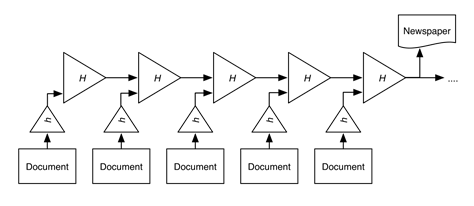
\includegraphics[width=0.7\textwidth]{./figs/hash-chain-with-data.png} 

		\caption{Hash chain with data.}		
		\label{fig:hash-chain-data}

	\end{center}	
\end{figure}

This approach, however, does not scale well with the number of documents
being logged. To address this, documents can be aggregated using data
structures like Merkle trees.

\subsubsection{Merkle Trees}\label{merkle-trees}

A Merkle tree, also known as a hash tree, is a binary tree data
structure in which every leaf node is the hash of a block of data, and
every non-leaf node is the hash of the concatenation of its children's
hashes (see \autoref{fig:merkle-tree}). This structure allows for efficient and secure verification of
the contents of large data sets.

\begin{figure}[t]
	%	\vspace{-0.3cm}
	\begin{center}
		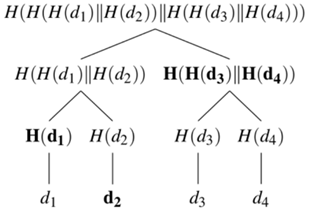
\includegraphics[width=0.5\textwidth]{./figs/merkle-tree.png} 

		\caption{Merkle tree.}		
		\label{fig:merkle-tree}

	\end{center}	
\end{figure}

The construction of a Merkle tree begins at the bottom with the leaf
nodes, which represent the hashes of individual data blocks, such as
transactions in a blockchain. These leaf nodes are then paired, and
their hashes are concatenated and hashed together to form the parent
nodes. This process is repeated recursively until a single root hash is
produced, which is known as the Merkle root.

The Merkle root has the unique property of representing the hash of the
entire data set. Any change to a single data block will result in a
different Merkle root, making it an effective tool for ensuring data
integrity.

One of the most significant advantages of Merkle trees is their ability
to provide \textbf{compact membership proofs}. A membership proof, also
known as an authentication path, allows a user to verify that a specific
piece of data is included in the data set without having to download and
hash the entire set. The proof consists of the leaf hash and the hashes
of the sibling nodes along the path from the leaf to the root. The
verifier can then use this information to reconstruct the Merkle root
and compare it to the known root hash. This process has a logarithmic
time and space complexity, making it highly efficient for large data
sets.

In the context of blockchains, Merkle trees are used to summarize all
the transactions in a block, producing a single Merkle root that is
included in the block header. This allows for efficient verification of
transactions without the need to download the entire block.

\subsubsection{A Combination of Merkle Trees and Hash Chains}\label{a-combination-of-merkle-trees-and-hash-chains}

Data can be aggregated in Merkle trees and added in batches (see \autoref{fig:combination}). The
integrity of the data is represented by the small root hashes, and the
integrity of the whole chain is represented by the last hash in the
chain.

\begin{figure}[t]
	%	\vspace{-0.3cm}
	\begin{center}
		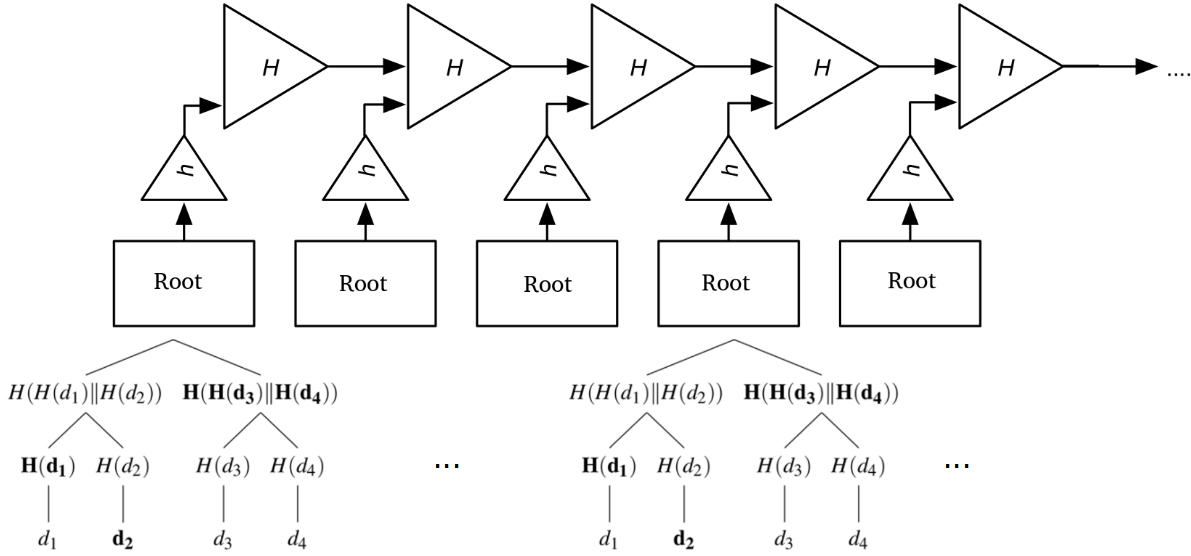
\includegraphics[width=0.9\textwidth]{./figs/combination-mk-hc.png} 

		\caption{A combination of Merkle tree and hash chains.}		
		\label{fig:combination}
	\end{center}	
\end{figure}


\subsubsection{Proof-of-Work (PoW)}\label{proof-of-work-pow}

Proof-of-Work is a mechanism that requires a significant amount of
computational work to be performed in order to achieve a certain goal (see example in \autoref{fig:pow}).
It is a key component of many cryptocurrencies, including Bitcoin.

A non-interactive version of PoW is \textbf{Hashcash}, proposed by Adam
Back in 1997 as a spam prevention mechanism. The idea is that the sender
of an email has to perform some work to send it, making it expensive to
send large volumes of spam. The proof generation is expensive, but the
verification is cheap.

\begin{figure}[!b]
	%	\vspace{-0.3cm}
	\begin{center}
		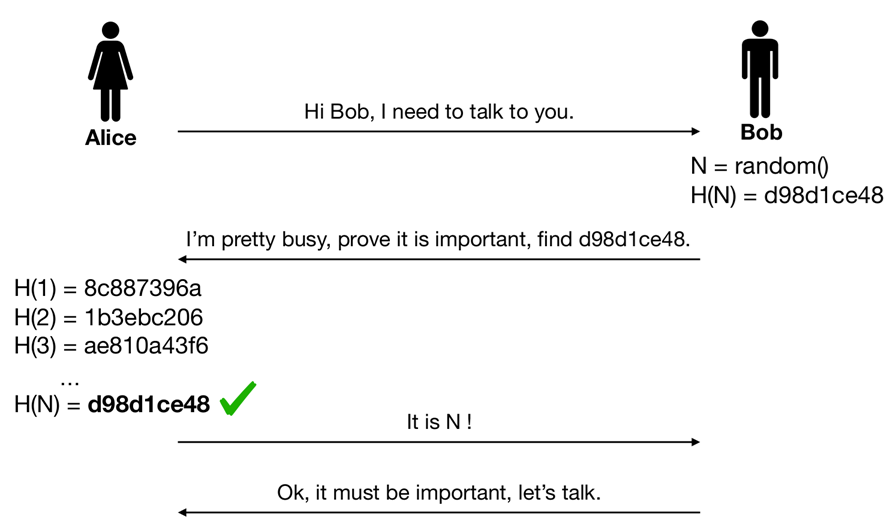
\includegraphics[width=0.8\textwidth]{./figs/pow.png} 
		\caption{Proof-of-Work principle.}		
		\label{fig:pow}
	\end{center}	
\end{figure}


\subsubsection{Commitments}\label{commitments}

A commitment scheme allows one to commit to a chosen value while keeping
it hidden from others, with the ability to reveal the committed value
later.

\begin{itemize}
	\tightlist
	\item
	\textbf{Commit}: Alice picks a value \texttt{x} and sends
	\texttt{H(x)} to Bob. This is the commitment. The use of a hash
	function guarantees the \textbf{binding} property (the commitment is
	bound to \texttt{x}), and since Bob doesn't know \texttt{x}, the
	\textbf{hiding} property is also satisfied.
	\item
	\textbf{Reveal}: Alice reveals \texttt{x} to Bob, who can then verify
	that \texttt{H(x)} matches the commitment he received.
\end{itemize}

\subsubsection{Digital Signatures}\label{digital-signatures}

Digital signatures are a cornerstone of modern cryptography, providing a
means to ensure the authenticity, integrity, and non-repudiation of
digital messages. They are the digital equivalent of a handwritten
signature, but with far stronger security guarantees. Digital signatures
are based on public-key cryptography, which involves a pair of
mathematically related keys: a private key, which is kept secret by the
owner, and a public key, which can be freely distributed.

The fundamental operations of a digital signature scheme are as follows:

\begin{itemize}
	\tightlist
	\item
	\textbf{Key Generation}: A user generates a key pair, consisting of a
	private key (SK) and a corresponding public key (PK).
	\item
	\textbf{Signing}: To sign a message, the user applies a signing
	algorithm to the message and their private key. This produces a
	digital signature, which is a fixed-size string of data (see \autoref{fig:signatures}.
	\item
	\textbf{Verification}: To verify a signature, a recipient uses the
	sender's public key, the message, and the signature. The verification
	algorithm returns a boolean value indicating whether the signature is
	valid (see \autoref{fig:signatures}.
\end{itemize}

\begin{figure}[t]
	%	\vspace{-0.3cm}
	\begin{center}
		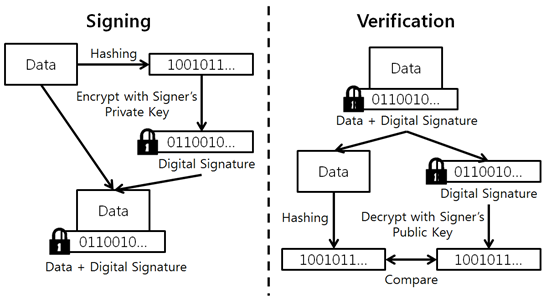
\includegraphics[width=0.7\textwidth]{./figs/signatures.png} 
		\caption{Digital signatures.}		
		\label{fig:signatures}
	\end{center}	
\end{figure}

Digital signatures provide several crucial security properties:

\begin{itemize}
	\tightlist
	\item
	\textbf{Authenticity}: A valid signature confirms that the message was
	signed by the owner of the corresponding private key. This is because
	only the owner of the private key could have produced a valid
	signature that can be verified with the public key.
	\item
	\textbf{Integrity}: The signature ensures that the message has not
	been altered since it was signed. Any modification to the message
	would result in an invalid signature.
	\item
	\textbf{Non-Repudiation}: The signer cannot plausibly deny having
	signed the message, as only they have access to the private key.
	However, it is important to note that this property can be challenged
	if the signer can plausibly claim that their private key was
	compromised.
	\item
	\textbf{Unforgeability}: It is computationally infeasible for an
	attacker to forge a valid signature for a new message without access
	to the private key. This property is based on the computational
	difficulty of the underlying mathematical problems, such as the
	discrete logarithm problem or the integer factorization problem.
\end{itemize}

In the context of blockchains, digital signatures are used to authorize
transactions. When a user wants to send cryptocurrency or interact with
a smart contract, they sign the transaction with their private key. This
signature proves that they are the legitimate owner of the funds or
assets being transferred and that they have authorized the transaction.

\begin{center}\rule{0.5\linewidth}{0.5pt}\end{center}

\subsection{Introduction to
	Blockchains}\label{section-3-introduction-to-blockchains}

\subsubsection{Why Blockchains?}\label{why-blockchains}

The advent of blockchain technology was driven by the inherent
limitations of traditional centralized information systems. These
systems, while ubiquitous, suffer from a number of vulnerabilities that
can compromise their security, reliability, and trustworthiness.

\begin{itemize}
	\tightlist
	\item
	\textbf{Single Point of Failure}: Centralized systems are susceptible
	to a single point of failure. A hardware malfunction, a software bug,
	or a successful denial-of-service (DDoS) attack on a central server
	can render the entire system inoperable.
	\item
	\textbf{Censorship}: A central authority has the power to censor users
	or transactions at its discretion, often without any mechanism for
	appeal or recourse. This can lead to arbitrary exclusion and a lack of
	fairness.
	\item
	\textbf{Limited Availability}: While cloud service providers often
	advertise high availability, achieving 100\% uptime is practically
	impossible in a centralized architecture. Outages can and do occur,
	leading to service disruptions.
	\item
	\textbf{Lack of Data Integrity}: In a centralized database, a
	malicious actor with sufficient privileges can alter or delete data
	without leaving a trace. This makes it difficult to guarantee the
	integrity and authenticity of the data.
	\item
	\textbf{Lack of Transparency}: The inner workings of centralized
	systems are often opaque to users. There is no way to independently
	verify that the system is operating as intended or that the data is
	being handled correctly.
\end{itemize}

Blockchain technology offers a paradigm shift, providing a decentralized
alternative that addresses these challenges through its inherent
properties:

\begin{itemize}
	\tightlist
	\item
	\textbf{Decentralization}: By distributing the ledger across a network
	of nodes, blockchains eliminate the single point of failure. The
	system can continue to operate even if some nodes go offline.
	\item
	\textbf{Censorship Resistance}: In a permissionless blockchain, all
	valid transactions are eventually processed. No single entity has the
	power to censor transactions, ensuring that the network remains open
	and accessible to all.
	\item
	\textbf{Immutability}: The append-only nature of the blockchain,
	enforced by cryptographic hashes, makes it extremely difficult to
	alter or delete past transactions. This creates a permanent and
	tamper-evident record of all activity on the network.
	\item
	\textbf{Auditability}: The entire history of the blockchain is
	available for anyone to inspect and verify. This allows for
	independent auditing of the system, ensuring that all transactions are
	valid and that the rules of the protocol have been followed.
	\item
	\textbf{Transparency}: All transactions on a public blockchain are
	visible to all participants. This transparency fosters trust and
	accountability, as all actions are open to scrutiny.
\end{itemize}

\subsubsection{3.2: High-Level View of
	Blockchains}\label{high-level-view-of-blockchains}

From a high-level perspective, a blockchain can be understood as a
synthesis of three distinct fields:

\begin{figure}[t]
	%	\vspace{-0.3cm}
	\begin{center}
		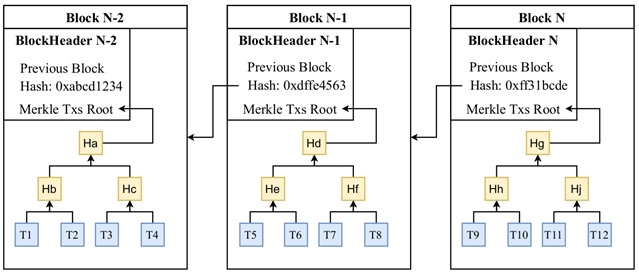
\includegraphics[width=0.8\textwidth]{./figs/blockchain-overview.png} 
		\caption{Overview of blockchain structure.}		
		\label{fig:overview-blockchain}
	\end{center}	
\end{figure}

\begin{itemize}
	\tightlist
	\item
	\textbf{Cryptography}: This provides the fundamental tools for
	securing the data and computations on the blockchain. As discussed in
	the previous section, cryptographic primitives such as hash functions
	and digital signatures are essential for ensuring the integrity,
	authenticity, and immutability of the ledger.
	\item
	\textbf{Distributed Systems}: This field provides the theoretical and
	practical foundations for building and maintaining a decentralized
	network. Blockchains are inherently distributed systems, and they rely
	on concepts from this field to address challenges such as fault
	tolerance, concurrency, and consensus.
	\item
	\textbf{Economics and Game Theory}: This provides the framework for
	designing protocols that incentivize rational actors to behave in a
	manner that is beneficial to the network as a whole. By carefully
	designing the economic incentives, it is possible to create a system
	that is robust and secure, even in the presence of self-interested or
	malicious participants.
\end{itemize}

At its core, a blockchain is a globally shared, append-only database, or
ledger, that is replicated across all participating nodes in the
network. The ledger is modified through the submission of transactions,
which are cryptographically signed by the participants. These
transactions are then bundled together into blocks, which are added to
the chain in a chronological and immutable manner. Each block is linked
to its predecessor by including the hash of the previous block's header,
creating a cryptographically secure chain of blocks that is resistant to
tampering (see \autoref{fig:overview-blockchain}).




\subsubsection{Participants in a Blockchain
	Network}\label{sec:participants-in-a-blockchain-network}

A blockchain network is a diverse ecosystem of participants, each with a
distinct role and level of engagement. The network can be conceptualized
as an inclusive hierarchy, with different types of nodes contributing to
the overall operation and security of the system (see \autoref{fig:participants}).

\begin{figure}[t]
	%	\vspace{-0.3cm}
	\begin{center}
		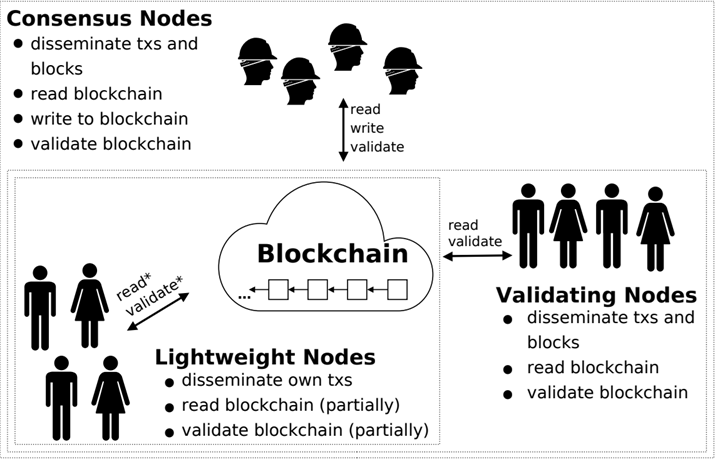
\includegraphics[width=0.8\textwidth]{./figs/participants.png} 
		\caption{Participants in blockchains.}		
		\label{fig:participants}
	\end{center}	
\end{figure}


\begin{itemize}
	\item
	\textbf{Consensus Nodes (Miners/Validators)}: At the top of the
	hierarchy are the consensus nodes, also known as miners in
	Proof-of-Work (PoW) systems or validators in Proof-of-Stake (PoS)
	systems. These nodes are the most active participants in the network,
	and they are responsible for the critical task of creating new blocks.
	This involves collecting and validating transactions, ordering them
	into a new block, and proposing the block to the rest of the network.
	In return for their efforts, consensus nodes are rewarded with newly
	created cryptocurrency and transaction fees.
	\item
	\textbf{Validating Nodes (Full Nodes)}: These nodes form the backbone
	of the network, providing a high level of security and
	decentralization. They download and store a complete copy of the
	blockchain, and they independently validate every transaction and
	block against the protocol's consensus rules. By doing so, they ensure
	that all participants are adhering to the same set of rules and that
	no invalid transactions are included in the ledger. Validating nodes
	also play a crucial role in disseminating transactions and blocks
	throughout the network.
	\item
	\textbf{Lightweight Nodes (Clients)}: These are the most common type
	of node, and they are typically used by end-users to interact with the
	blockchain. Lightweight nodes, as their name suggests, do not store
	the entire blockchain. Instead, they only download and store the block
	headers, which contain a summary of the block's contents, including
	the Merkle root. To verify a transaction, a lightweight node can
	request a membership proof from a full node, which allows it to
	confirm that the transaction is included in a block without having to
	download the entire block. This makes lightweight nodes ideal for use
	on devices with limited storage and bandwidth, such as mobile phones.
\end{itemize}

\subsubsection{How Participants
	Communicate}\label{how-participants-communicate}

Participants in a blockchain network communicate through a peer-to-peer
(P2P) network over-layed over underlying network using a gossiping protocol (see \autoref{fig:network-overlay}). Messages are sent only to a
small number of peers (e.g., 8-50). When a new node joins the network,
it scans a list of hard-coded directory nodes (DNS seeders) to find
peers.

The network propagation delay is a crucial factor. A 2013 study on
Bitcoin showed that the mean time for a block to be seen by 95\% of the
nodes was 12.6 seconds, with a maximum of 40 seconds \ih{cite}.

\begin{figure}[t]
	%	\vspace{-0.3cm}
	\begin{center}
		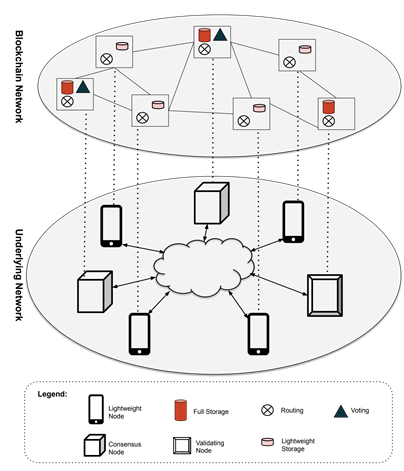
\includegraphics[width=0.4\textwidth]{./figs/network-overlay.png} 
		\caption{Overview of network in blockchains.}		
		\label{fig:network-overlay}
	\end{center}	
\end{figure}

\begin{center}\rule{0.5\linewidth}{0.5pt}\end{center}

\subsection{Summary / Key Takeaways}\label{summary-key-takeaways}

This section has provided a comprehensive introduction to the BDA
course, outlining its objectives, structure, and the expertise of its
instructors. It has underscored the critical importance of a strong
technical foundation in the principles of blockchain and decentralized
applications. The section has delved into the essential cryptographic
constructs that form the bedrock of blockchain technology, including:

\begin{itemize}
	\tightlist
	\item
	\textbf{Cryptographic Hash Functions}: Their properties of pre-image
	resistance, second pre-image resistance, and collision resistance are
	fundamental to the integrity and security of the blockchain.
	\item
	\textbf{Hash Chains}: A simple yet powerful method for creating
	sequences of verifiable data, with applications such as one-time
	passwords.
	\item
	\textbf{Merkle Trees}: An efficient data structure for summarizing and
	verifying the integrity of large sets of data, enabling compact
	membership proofs.
	\item
	\textbf{Digital Signatures}: The mechanism for providing authenticity,
	integrity, and non-repudiation in a decentralized environment.
\end{itemize}

The section concluded with a high-level overview of blockchain
technology, highlighting its key features and the problems it aims to
solve. It also provided a classification of the different participants
in a blockchain network, from lightweight clients to consensus nodes.

\begin{center}\rule{0.5\linewidth}{0.5pt}\end{center}

\subsection{Keywords}\label{keywords}

\begin{itemize}
	\tightlist
	\item
	\textbf{Blockchain}: A decentralized, distributed, and immutable
	digital ledger that is used to record transactions across many
	computers so that any involved record cannot be altered retroactively,
	without the alteration of all subsequent blocks.
	\item
	\textbf{Decentralized Application (DApp)}: An application that is run
	by many users on a decentralized network with trustless protocols.
	They are designed to avoid any single point of failure.
	\item
	\textbf{Cryptographic Hash Function}: A mathematical algorithm that
	maps data of arbitrary size to a bit string of a fixed size (a hash)
	and is a one-way function, that is, a function which is practically
	infeasible to invert.
	\item
	\textbf{Merkle Tree}: A tree in which every leaf node is labelled with
	the cryptographic hash of a data block, and every non-leaf node is
	labelled with the cryptographic hash of the labels of its child nodes.
	\item
	\textbf{Digital Signature}: A mathematical scheme for demonstrating
	the authenticity of digital messages or documents. A valid digital
	signature gives a recipient very strong reason to believe that the
	message was created by a known sender (authentication), that the
	sender cannot deny having sent the message (non-repudiation), and that
	the message was not altered in transit (integrity).
	\item
	\textbf{Consensus Protocol}: A set of rules and procedures that allows
	a distributed network of computers to work together to achieve a
	common goal. In the context of blockchains, the consensus protocol is
	what allows the network to agree on the state of the ledger.
	\item
	\textbf{Attacker Model}: A formal model of the capabilities of an
	attacker, used to analyze the security of a system.
	\item
	\textbf{Proof-of-Work (PoW)}: A consensus mechanism that requires a
	significant amount of computational work to be performed in order to
	create a new block.
	\item
	\textbf{Proof-of-Stake (PoS)}: A consensus mechanism in which the
	creator of the next block is chosen in a deterministic way, depending
	on its wealth, also defined as stake.
\end{itemize}

\begin{center}\rule{0.5\linewidth}{0.5pt}\end{center}

\subsection{Further Reading}\label{further-reading}

\begin{itemize}
	\tightlist
	\item
	\textbf{Bitcoin and Cryptocurrency Technologies}:\\
	\url{http://bitcoinbook.cs.princeton.edu/}
	\item
	\textbf{Security Reference Architecture for Blockchains}:\\
	\url{https://ieeexplore.ieee.org/document/9239372}
	\item
	\textbf{Blockchain Technology Course by P. Szalachowski}:\\
	\url{https://github.com/pszal/teaching/tree/master/Blockchain-Technology}
\end{itemize}
\newpage

\section{Consensus Protocols \& Blockchains}\label{sec:consensus-protocols-blockchains}
%\subsection{Introduction}\label{in/troduction}

This section delves into the fundamental mechanisms that underpin the
operation of decentralized networks: consensus protocols. These
protocols are the cornerstone of any blockchain, as they provide the
means for a distributed network of independent and potentially
untrusting nodes to reach an agreement on the state of the ledger. As we
will learn, achieving this ``agreement'' or ``consensus'' in a
decentralized environment is a non-trivial challenge, especially when
considering the potential for network delays, failures, and even
malicious participants.

We will begin by exploring the theoretical foundations of consensus,
including the different types of blockchain networks and how they manage
access and participation. We will dissect the inherent trade-offs in
distributed systems as encapsulated by the famous CAP theorem, and
understand why blockchains must often prioritize availability and
partition tolerance, leading to a model of ``eventual consistency.'' We
will also define the critical properties that a robust consensus
protocol must satisfy -- namely \textbf{safety, liveness, and finality} -- to
ensure the network remains secure and functional.

The section will then proceed to examine the two primary paradigms for
achieving consensus: \textbf{lottery-based} and \textbf{voting-based} mechanisms. We will
analyze the respective strengths and weaknesses of each approach,
considering factors such as scalability, network overhead, and the time
it takes for transactions to be irreversibly confirmed. A significant
portion of the section will be dedicated to understanding the concept of
\textbf{forks} -- a natural consequence of the probabilistic nature of some
consensus protocols -- and the mechanisms used to resolve them.

Furthermore, we will explore the classic \textbf{Byzantine Generals Problem},
which provides a powerful analogy for understanding the challenges of
achieving consensus in the presence of malicious actors. This will lead
to a discussion of Byzantine Fault Tolerance (BFT) and its practical
implementation in the form of the Practical Byzantine Fault Tolerance
(PBFT) algorithm, a protocol foundational to many permissioned
blockchains.

Finally, we will examine the most prominent consensus protocols used in
practice today. This includes Proof-of-Work (PoW), the original,
resource-intensive mechanism of Bitcoin; Proof-of-Stake (PoS), a more
energy-efficient alternative that has been adopted by many modern
blockchains like Ethereum; and \textbf{Proof-of-Authority} (PoA), a
reputation-based mechanism well-suited for private, permissioned
networks. We will also discuss the crucial role of incentive schemes in
securing permissionless networks and the complex challenges of managing
decentralized names and identities.

\subsection{Learning Objectives}\label{learning-objectives}

\begin{itemize}
	\tightlist
	\item
	Understand the different types of blockchain networks (permissionless,
	permissioned, and semi-permissionless) and their methods for
	controlling entry and preventing Sybil attacks.
	\item
	Grasp the concepts of the CAP theorem and its implications for
	blockchain design, particularly the trade-off between consistency and
	availability.
	\item
	Learn the standard goals of consensus protocols: safety (agreement),
	liveness (termination), and finality (eventual consistency).
	\item
	Differentiate between lottery-based and voting-based consensus
	mechanisms and their respective trade-offs.
	\item
	Understand the concept of forks (accidental, malicious, and
	intentional) and the fork-choice rules used to resolve them.
	\item
	Gain insight into the Byzantine Generals Problem and its relevance to
	fault tolerance in distributed systems.
	\item
	Learn about specific consensus protocols, including Practical
	Byzantine Fault Tolerance (PBFT), Proof-of-Work (PoW), and
	Proof-of-Stake (PoS).
	\item
	Understand the role of incentive schemes in motivating honest
	participation in blockchain networks.
	\item
	Understand the challenges of decentralized identity management as
	described by Zooko's Triangle.
\end{itemize}

\begin{center}\rule{0.5\linewidth}{0.5pt}\end{center}

\subsection{Blockchain Networks and System
	Models}\label{section-1-blockchain-networks-and-system-models}

\subsubsection{Types of Blockchains}\label{types-of-blockchains}

Blockchains can be broadly classified into three categories based on
their access control mechanisms, which determine how new nodes can join
the network and participate in the consensus process.

\begin{itemize}
	\item
	\textbf{Permissionless Blockchains}: These are open networks that
	anyone can join without requiring permission from a central authority.
	The core challenge in such a system is the \textbf{Sybil attack},
	where an attacker could create a large number of pseudonymous
	identities to gain a disproportionate influence on the network. 
%	As the 	lecturer explained, 
	If consensus were to be based on a simple vote, one
	could ``create a thousand fake identities and have a thousand votes.''
	To prevent this, permissionless blockchains employ
	\textbf{Proof-of-Resource} mechanisms. These mechanisms require nodes
	to demonstrate ownership of a scarce resource, such as computational
	power (in Proof-of-Work) or a significant financial stake (in
	Proof-of-Stake). A node's influence in the consensus process is
	directly proportional to the amount of the scarce resource it
	controls, not the number of identities it possesses. Bitcoin and
	Ethereum are prominent examples of permissionless blockchains.
	\item
	\textbf{Permissioned Blockchains}: In contrast to permissionless
	blockchains, these are closed networks where new nodes must obtain
	explicit permission to join from a centralized or federated authority.
	This authority is responsible for vetting and onboarding new
	participants. For instance, a bank operating its own blockchain would
	only allow vetted entities to join. Because participants are known and
	there's a mechanism to expel malicious actors, the risk of Sybil
	attacks is eliminated. This allows permissioned blockchains to use
	more traditional and efficient voting-based consensus protocols, such
	as Practical Byzantine Fault Tolerance (PBFT), where each node
	typically has an equal say (``one node, one vote''). These networks
	are well-suited for enterprise applications where privacy, control,
	and performance are paramount.
	\item
	\textbf{Semi-Permissionless Blockchains}: This category represents a
	hybrid approach, analogous to a joint-stock company where voting power
	is tied to ownership. While new nodes do not require permission from a
	central authority to join, they must acquire a ``stake'' in the
	network to participate in the consensus process. This stake, which is
	typically in the form of the network's native cryptocurrency, can be
	acquired from any existing participant. A node's consensus power is
	proportional to the size of its stake, which serves as a form of
	collateral that can be forfeited in the event of malicious behavior.
	This model aims to strike a balance between the openness of
	permissionless networks and the control of permissioned networks.
\end{itemize}

\subsubsection{Centralized vs.~Decentralized
	Systems}\label{centralized-vs.-decentralized-systems}

In the discourse surrounding blockchain technology, the terms
``distributed'' and ``decentralized'' are often used interchangeably,
but they refer to distinct concepts. A clear understanding of this
distinction is essential for appreciating the unique value proposition
of blockchains.

\begin{itemize}
	\item
	\textbf{Distributed Systems}: A distributed system (see \autoref{fig:distrib-decentralized}) is one in which
	components are located on different networked computers, which then
	communicate and coordinate their actions. The key characteristic of a
	distributed system is its \textbf{geographical distribution}. For
	example, a company like Google operates a massive distributed system
	with data centers located all over the world. However, despite its
	distributed nature, this system is still \textbf{centrally controlled}
	by a single entity.
	\item
	\textbf{Decentralized Systems}: A decentralized system, on the other
	hand, is defined by its \textbf{control and trust model}. In a fully
	decentralized system, there is no single point of control or trust.
	Instead, control is distributed among the participants, and decisions
	are made through a consensus mechanism. This eliminates the need for a
	trusted third party, as the system is designed to be resilient to the
	failure or malicious behavior of individual nodes.
\end{itemize}

While all decentralized systems are necessarily distributed, the
converse is not true. A system can be geographically distributed but
still be centrally controlled. The true innovation of blockchain
technology lies in its ability to create a fully decentralized system
that can operate in a trustless environment.

\begin{figure}[t]
	%	\vspace{-0.3cm}
	\begin{center}
		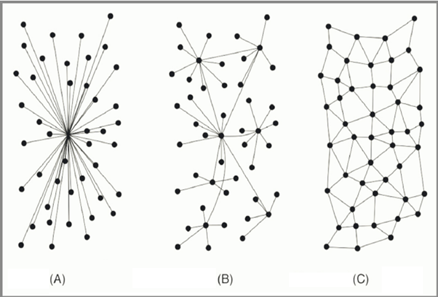
\includegraphics[width=0.8\textwidth]{./figs/distrib-decentralized.png} 
		\caption{(A) centralized system, (B) partially decentralized system, (C) fully decentralized system.}		
		\label{fig:distrib-decentralized}
	\end{center}	
\end{figure}

\subsubsection{The CAP Theorem}\label{the-cap-theorem}

The CAP theorem, also known as Brewer's theorem, is a fundamental
principle in distributed systems that describes an inherent trade-off
between three desirable properties: consistency, availability, and
partition tolerance. The theorem states that any distributed data store
can only provide two of these three guarantees simultaneously.

\begin{itemize}
	\tightlist
	\item
	\textbf{Consistency}: This guarantee ensures that all nodes in the
	network see the same data at the same time. In a consistent system,
	every read operation will return the value of the most recent write
	operation or an error.
	\item
	\textbf{Availability}: This guarantee ensures that every request to
	the system receives a response, without the guarantee that it contains
	the most recent write. In an available system, there are no single
	points of failure, and the system remains operational even if some
	nodes are down.
	\item
	\textbf{Partition Tolerance}: This guarantee ensures that the system
	continues to operate even if the network is partitioned, meaning that
	messages between nodes are dropped or delayed.
\end{itemize}

In the context of blockchain technology, which operates over the public
internet, network partitions are an unavoidable reality. Therefore, any
blockchain protocol \textbf{must be partition tolerant}. This leaves a
fundamental choice between consistency and availability.
%
Most blockchain protocols, particularly those based on Nakamoto
consensus, prioritize \textbf{availability and partition tolerance} over
strong consistency. This means that they will continue to operate and
process transactions even in the presence of network partitions, but at
the cost of immediate consistency. Instead, they offer a weaker form of
consistency known as \textbf{eventual consistency}. This means that
while different nodes may have a different view of the ledger at any
given moment, they will eventually converge on a single, consistent
state over time. This is typically achieved by requiring a certain
number of \textbf{confirmations} (i.e., subsequent blocks) before a
transaction is considered final. For example, in Bitcoin, a transaction
is conventionally considered secure and final after six confirmations,
which takes approximately 60 minutes.

\begin{figure}[t]
	%	\vspace{-0.3cm}
	\begin{center}
		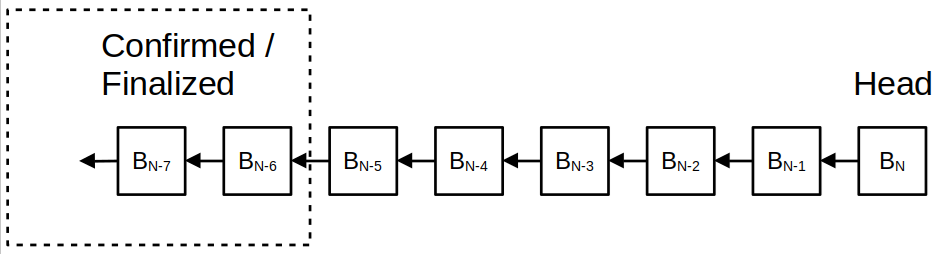
\includegraphics[width=0.8\textwidth]{./figs/btc-finality.png} 
		\caption{Eventual consistency of availability-favored blockchains within CAP theorem.}		
		\label{fig:btc-finality}
	\end{center}	
\end{figure}

\begin{center}\rule{0.5\linewidth}{0.5pt}\end{center}

\subsection{Consensus Protocols in
	Blockchains}\label{section-2-consensus-protocols-in-blockchains}

\subsubsection{Goals of Consensus
	Protocols}\label{goals-of-consensus-protocols}

Consensus protocols are the mechanisms by which a distributed network of
nodes can agree on a single, consistent history of transactions. These
protocols are designed to achieve several key goals, which are essential
for the secure and reliable operation of a blockchain.

\begin{itemize}
	\item
	\textbf{Safety (Agreement)}: This property ensures that all honest
	nodes in the network will eventually agree on the same value. In the
	context of a blockchain, this means that all honest nodes will have an
	identical copy of the ledger. Safety is a critical property, as it
	prevents a ``split-brain'' scenario where different parts of the
	network have conflicting views of the truth.
	\item
	\textbf{Liveness (Termination)}: This property ensures that the
	network will continue to make progress. In other words, all honest
	nodes will eventually decide on a value, and the blockchain does not
	stall. This ensures that new transactions are eventually included in
	the ledger.
	\item
	\textbf{Finality}: This is a concept that reinterprets safety and
	liveness in the context of blockchains that provide eventual
	consistency. A block is said to have reached finality when it is
	computationally infeasible for it to be overturned or removed from the
	blockchain (see \autoref{fig:btc-finality}). The time to finality can vary significantly between
	different consensus protocols. For example, in Bitcoin, a block is
	typically considered final after six subsequent blocks have been added
	to the chain, which takes approximately one hour. In contrast, some
	voting-based protocols can achieve finality in a matter of seconds.
\end{itemize}

\subsubsection{Lottery vs.~Voting}\label{lottery-vs.-voting}

At a high level, consensus protocols can be categorized into two main
approaches: lottery-based and voting-based~\cite{hyperledger1}.

\begin{itemize}
	\item
	\textbf{Lottery-Based Consensus}: In this approach, a single node is
	selected through a lottery-like mechanism to be the leader for a given
	round. This leader is then responsible for producing the next block
	and broadcasting it to the network. The probability of being selected
	as the leader is typically proportional to the amount of a scarce
	resource that a node controls, such as computational power in
	Proof-of-Work or stake in Proof-of-Stake. Lottery-based protocols are
	characterized by their low network overhead and high scalability, as
	they do not require all nodes to communicate with each other. However,
	they are susceptible to forks, which can occur if multiple leaders are
	elected simultaneously and propose conflicting blocks.
	\item
	\textbf{Voting-Based Consensus}: In this approach, all nodes in the
	network participate in a collective voting process to agree on the
	next block. This typically involves multiple rounds of communication,
	where nodes exchange messages to reach a consensus. Voting-based
	protocols, such as PBFT, offer the advantage of low-latency finality,
	as a block is considered final once it has been approved by a
	sufficient number of nodes. However, they suffer from high
	communication complexity, which is typically on the order of
	$O(N^2)$, where $N$ is the number of nodes. This makes them unsuitable
	for large, permissionless networks, but well-suited for smaller,
	permissioned blockchains where the number of participants is limited.
\end{itemize}

Many modern protocols, like Algorand~\cite{gilad2017algorand}, use a combination of these two
approaches, using a lottery to select a small committee of nodes which
then vote on the next block.

\subsubsection{Forks}\label{forks}

A fork is a situation where a blockchain diverges into two or more
competing chains. This can happen for a variety of reasons, and it is a
fundamental concept to understand in the context of blockchain
technology.

\begin{itemize}
	\item
	\textbf{Accidental Forks}: These are a natural consequence of the
	probabilistic nature of lottery-based consensus protocols. Due to
	network latency, it is possible for two or more nodes to solve the
	consensus puzzle at approximately the same time and broadcast their
	new blocks to the network. This can result in a temporary fork, where
	different parts of the network have a different view of the latest
	block. These forks are typically resolved quickly as subsequent blocks
	are added to one of the chains, making it the longest and therefore
	the canonical chain.
	\item
	\textbf{Malicious Forks}: These are intentionally created by attackers
	with the aim of disrupting the network or defrauding other users. A
	common example is a \textbf{double-spending attack}, where an attacker
	sends a transaction to a merchant, waits for the merchant to deliver
	the goods, and then creates a fork to reverse the transaction. Another
	example is \textbf{selfish mining}, where a miner with significant
	hash power secretly builds a longer chain and then releases it to the
	network to orphan the blocks of other miners and claim their rewards.
	\item
	\textbf{Intentional Forks (Hard Forks and Soft Forks)}: These are
	planned forks that are created to introduce changes to the protocol.
	
	\begin{itemize}
		\tightlist
		\item
		A \textbf{hard fork} is a backward-incompatible change to the
		protocol, which requires all nodes to upgrade to the new version. If
		some nodes do not upgrade, the blockchain will permanently split
		into two separate chains. The creation of Bitcoin Cash from Bitcoin,
		which increased the block size limit, is a well-known example of a
		hard fork.
		\item
		A \textbf{soft fork} is a backward-compatible change, which allows
		non-upgraded nodes to continue to participate in the network.
	\end{itemize}
\end{itemize}

Forks are typically resolved through a \textbf{fork-choice rule}, which
is a set of rules that nodes use to determine which chain to consider
the canonical one. The most common fork-choice rule is the
\textbf{longest chain rule}, which states that the valid chain is the
one with the most blocks (see \autoref{fig:longest-chain}), as it represents the most accumulated work.
Another approach is the \textbf{strongest chain rule}, which takes into
account the ``quality'' of the blocks, such as the total number of
transactions they contain.

\begin{figure}[t]
	%	\vspace{-0.3cm}
	\begin{center}
		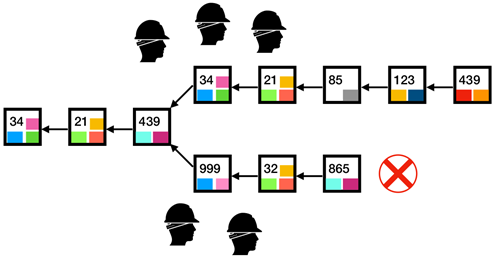
\includegraphics[width=0.8\textwidth]{./figs/longest-chain.png} 
		\caption{Longest chain fork-choice rule.}		
		\label{fig:longest-chain}
	\end{center}	
\end{figure}

\begin{center}\rule{0.5\linewidth}{0.5pt}\end{center}

\subsection{Byzantine Fault
	Tolerance}\label{section-3-byzantine-fault-tolerance}

\subsubsection{The Byzantine Generals
	Problem}\label{the-byzantine-generals-problem}

The Byzantine Generals Problem is a classic thought experiment in
distributed computing that provides a powerful analogy for the
challenges of achieving consensus in a network where some participants
may be unreliable or malicious. The problem is typically stated as
follows (see also \autoref{fig:generals}):

\begin{itemize}
	\item \textit{A group of Byzantine generals are besieging a city. They must decide whether to attack or retreat. If all loyal generals attack, they
		will be victorious. If all loyal generals retreat, they will be saved.
		However, if some generals attack while others retreat, they will be
		defeated. The generals can only communicate with each other via
		messengers, and some of the generals may be traitors who will try to
		disrupt the plan by sending conflicting messages.}
	
\end{itemize}

\begin{figure}[t]
	%	\vspace{-0.3cm}
	\begin{center}
		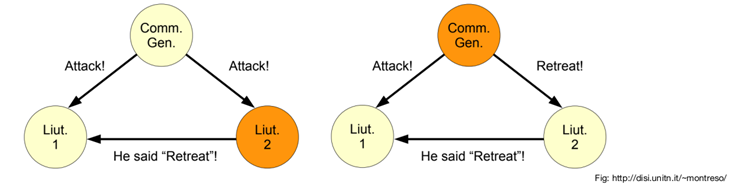
\includegraphics[width=0.9\textwidth]{./figs/byzantyne-generals.png}
		\caption{Byzantine generals problem.}		
		\label{fig:generals}
	\end{center}	
\end{figure}


The problem illustrates the difficulty of achieving consensus in a
distributed system where there is no central authority and where some
nodes may be faulty or malicious. A loyal general receiving conflicting
messages -- for instance, ``attack'' from the commander but ``retreat''
from a fellow lieutenant -- cannot know who the traitor is.

It has been proven that a solution to the Byzantine Generals Problem is
only possible if the number of loyal generals is greater than two-thirds
of the total number of generals. In other words, a system can tolerate
\texttt{f} Byzantine nodes only if the total number of nodes \texttt{N}
is greater than \texttt{3f} (\texttt{f\ \textless{}\ N/3}). This means
that more than two-thirds of the nodes must be honest and follow the
protocol for the system to be able to reach a consensus. This result has
profound implications for the design of fault-tolerant distributed
systems, including blockchains.

\subsubsection{Practical Byzantine Fault Tolerance
	(PBFT)}\label{practical-byzantine-fault-tolerance-pbft}

Practical Byzantine Fault Tolerance (PBFT) \ih{cite} is a landmark consensus
protocol designed to be resilient to Byzantine failures in asynchronous
systems. Developed by Miguel Castro and Barbara Liskov in 1999, PBFT
provides a practical solution to the Byzantine Generals Problem, making
it suitable for use in real-world distributed systems.

PBFT is a voting-based protocol that operates in a series of rounds,
with each round having a designated leader. The protocol involves a
multi-step process to ensure that all honest nodes agree on the order of
operations before they are committed to the ledger. The key phases of
the PBFT protocol are (see also \autoref{fig:pbft}):

\begin{enumerate}
	\def\labelenumi{\arabic{enumi}.}
	\tightlist
	\item
	\textbf{Request}: A client sends a request to the leader node.
	\item
	\textbf{Pre-prepare}: The leader node multicasts the request to all
	other nodes in the network.
	\item
	\textbf{Prepare}: Upon receiving the pre-prepare message, each node
	verifies the request and, if it is valid, multicasts a prepare message
	to all other nodes.
	\item
	\textbf{Commit}: A node waits until it has received \texttt{2f}
	prepare messages from different nodes that match the pre-prepare
	message. At this point, the node multicasts a commit message to all
	other nodes.
	\item
	\textbf{Reply}: A node waits until it has received \texttt{2f\ +\ 1}
	commit messages from different nodes. At this point, the node executes
	the request and sends a reply to the client.
\end{enumerate}

The client waits for \texttt{f\ +\ 1} replies from different nodes with
the same result. This ensures that the result is valid, as at most
\texttt{f} nodes can be malicious.

PBFT is well-suited for permissioned blockchains where the number of
participants is relatively small, due to its $O(N^2)$ communication
complexity. Its ability to provide low-latency finality makes it an
attractive choice for enterprise applications that require high
performance and strong consistency guarantees.

\begin{figure}[t]
	%	\vspace{-0.3cm}
	\begin{center}
		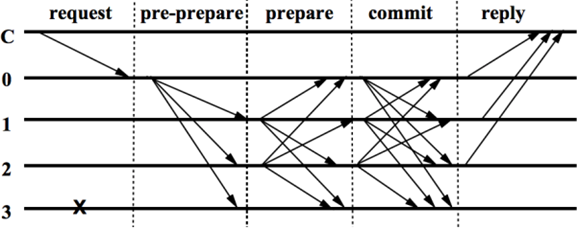
\includegraphics[width=0.75\textwidth]{./figs/pbft.png}
		\caption{Practical Byzantine Fault Tolerant protocol.}		
		\label{fig:pbft}
	\end{center}	
\end{figure}

\begin{center}\rule{0.5\linewidth}{0.5pt}\end{center}

\subsection{Section 4: Consensus Protocols in
	Practice}\label{section-4-consensus-protocols-in-practice}

\subsubsection{Proof-of-Work (PoW)}\label{sec:proof-of-work-pow}

Proof-of-Work (PoW) is the pioneering consensus mechanism that was first
introduced with Bitcoin~\cite{nakamoto2008bitcoin}. It is a permissionless, lottery-based protocol
that allows a decentralized network to reach a consensus without relying
on a central authority.

In a PoW system, nodes, known as miners, compete to solve a
computationally intensive puzzle. This puzzle involves finding a value,
called a nonce, which, when combined with the data in the block and
hashed, produces a hash that is below a certain target value. The
difficulty of this puzzle is adjusted periodically to ensure that a new
block is created at a relatively constant rate (approximately every 10
minutes for Bitcoin), regardless of the total computational power of the
network.

The first miner to find a valid nonce is rewarded with a certain amount
of cryptocurrency, known as the block reward, as well as the transaction
fees from the transactions included in the block. This economic
incentive motivates miners to contribute their computational resources
to the network, thereby securing the blockchain.

PoW is highly scalable in terms of the number of participating nodes, as
anyone can become a miner by simply dedicating computational resources
to the network. However, it has been widely criticized for its high
energy consumption, as the mining process requires a vast amount of
electricity, comparable to that of entire countries. This has led to the
development of alternative consensus mechanisms, such as Proof-of-Stake,
which are more energy-efficient.

\subsubsection{Proof-of-Stake (PoS)}\label{proof-of-stake-pos}

Proof-of-Stake (PoS) is a class of consensus mechanisms that has emerged
as a more energy-efficient alternative to Proof-of-Work. In a PoS
system, the right to create a new block is not determined by a
computational race, but by the amount of cryptocurrency that a node
holds and is willing to ``stake'' as collateral.

The fundamental principle of PoS is that nodes with a larger stake have
a higher probability of being selected to create the next block. This is
because they have a greater vested interest in the security and
integrity of the network. If a validator attempts to add a fraudulent
block to the chain, they risk losing their stake (a process known as
``slashing''), which serves as a powerful economic disincentive against
malicious behavior.

PoS offers several advantages over PoW, including improved energy
efficiency, lower barriers to entry for validators, and the ability to
achieve faster finality. However, it also introduces new challenges,
such as the ``nothing at stake'' problem, where validators have an
incentive to vote for multiple conflicting chains, and the potential for
centralization if a small number of entities accumulate a large portion
of the stake \ih{ref on later}.

\subsubsection{Proof-of-Authority
	(PoA)}\label{proof-of-authority-poa}

Proof-of-Authority (PoA) is a reputation-based consensus mechanism that
is designed for permissioned blockchains. In a PoA network, new nodes
must be approved by a central or federated authority to become
validators. Instead of staking computational resources or
cryptocurrency, validators in a PoA network stake their reputation.

The core idea behind PoA is that validators are incentivized to act
honestly to maintain their reputation. If a validator is found to be
malicious, they can be removed from the network, and their reputation
will be tarnished. This makes PoA a suitable choice for private or
consortium blockchains where the participants are known and trusted
entities, such as a group of financial institutions or a consortium of
universities.

PoA offers several advantages over other consensus mechanisms, including
high throughput, low transaction costs, and energy efficiency. However,
it is also more centralized than permissionless consensus mechanisms
like PoW and PoS, as the authority to validate transactions is
concentrated in a small group of approved nodes.

\begin{center}\rule{0.5\linewidth}{0.5pt}\end{center}


\subsection{Incentive Schemes and Decentralized
	Identities}\label{section-5-incentive-schemes-and-decentralized-identities}

%\subsubsection{Incentive Schemes}\label{incentive-schemes}

Incentive schemes are a critical component of permissionless and
semi-permissionless blockchains, as they provide the economic motivation
for nodes to participate in the consensus process and act honestly.
These schemes typically consist of two main components:

\begin{itemize}
	\tightlist
	\item
	\textbf{Block Rewards}: These are newly created units of
	cryptocurrency that are awarded to the node that successfully creates
	a new block. Block rewards serve as the primary incentive for miners
	in a PoW system and validators in a PoS system.
	\item
	\textbf{Transaction Fees}: These are small fees that are paid by users
	to have their transactions included in a block. Transaction fees
	provide an additional incentive for consensus nodes and become
	increasingly important as the block reward diminishes over time.
	Moreover, transaction fees create the market for the speed of inclusion of transactions in the blockchains -- the higher the fee, the faster inclusion of transaction.
\end{itemize}

The design of the incentive scheme is crucial for the security and
stability of the blockchain. Misaligned incentives can create
vulnerabilities that can be exploited by attackers. For example, if the
transaction fees are too low, miners may be incentivized to create empty
blocks, which can reduce the overall utility of the network.

\subsubsection{Decentralized Names \&
	Identities}\label{decentralized-names-identities}

The management of names and identities in a decentralized system
presents a unique set of challenges. In a traditional centralized
system, a central authority is responsible for managing identities and
ensuring that names are unique. In a decentralized system, however,
there is no such authority, which can lead to problems such as name
collisions and Sybil attacks.

\medskip
\textbf{Zooko's Triangle} is a well-known conjecture in computer science
that illustrates the trade-off among three desirable properties of a
naming system:

\begin{itemize}
	\tightlist
	\item
	\textbf{Human-meaningful}: The names should be easy for humans to
	remember and use (e.g., ``google.com'').
	\item
	\textbf{Secure}: The names should be resistant to spoofing and other
	forms of attack, meaning a name correctly resolves to its intended
	entity.
	\item
	\textbf{Decentralized}: The system should not rely on a central
	authority for name resolution.
\end{itemize}

\begin{figure}[t]
	%	\vspace{-0.3cm}
	\begin{center}
		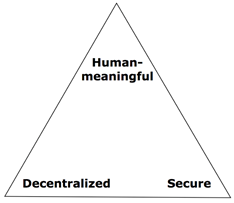
\includegraphics[width=0.3\textwidth]{./figs/zooko.png}
		\caption{Zooko's triangle.}		
		\label{fig:zooko}
	\end{center}	
\end{figure}

Zooko's Triangle posits that it is difficult to achieve all three of
these properties simultaneously. For example, DNS is human-meaningful
and secure (with DNSSec) but centralized. Onion addresses in Tor are
secure and decentralized but not human-meaningful. It is believed that
blockchain technology can help to relax this trade-off by providing a
secure and decentralized platform for managing names and identities.

\textbf{Namecoin} was one of the first projects to attempt to create a
decentralized naming system on a blockchain. It is a fork of Bitcoin
that allows users to register key-value pairs in a censorship-resistant
manner, creating a decentralized domain name system (DNS) with the
top-level domain \texttt{.bit}. However, Namecoin has been plagued by
problems such as \textbf{cyber-squatting} (where users register names
they do not own with the intention of selling them) and
\textbf{front-running} (where an attacker sees a registration
transaction and quickly submits their own for the same name with a
higher fee).

\begin{center}\rule{0.5\linewidth}{0.5pt}\end{center}

\subsection{Summary / Key Takeaways}\label{summary-key-takeaways}

This section has provided a comprehensive exploration of consensus
protocols, the foundational mechanisms that enable the secure and
reliable operation of blockchain networks. We have examined the key
concepts and trade-offs that underpin the design of these protocols,
including:

\begin{itemize}
	\tightlist
	\item
	\textbf{Types of Blockchains}: We have distinguished between
	permissionless, permissioned, and semi-permissionless blockchains,
	highlighting the different access control models and their
	implications for security and decentralization.
	\item
	\textbf{The CAP Theorem}: We have explored the fundamental trade-off
	between consistency, availability, and partition tolerance in
	distributed systems, and how this theorem shapes the design of
	blockchain protocols, leading to eventual consistency.
	\item
	\textbf{Goals of Consensus}: We have defined the key properties of a
	robust consensus protocol: safety, liveness, and finality.
	\item
	\textbf{Lottery vs.~Voting}: We have contrasted the two primary
	approaches to achieving consensus, analyzing their respective
	advantages and disadvantages in terms of scalability, network
	overhead, and time to finality.
	\item
	\textbf{Byzantine Fault Tolerance}: We have delved into the classic
	Byzantine Generals Problem and its solution in the form of Byzantine
	Fault Tolerance, which is essential for building systems that are
	resilient to malicious actors, requiring
	\texttt{N\ \textgreater{}\ 3f} nodes.
	\item
	\textbf{Consensus in Practice}: We have examined the most prominent
	consensus protocols used in real-world blockchains, including
	Proof-of-Work, Proof-of-Stake, and Proof-of-Authority.
	\item
	\textbf{Incentive Schemes and Decentralized Identities}: We have
	discussed the importance of economic incentives in securing blockchain
	networks and the challenges of managing names and identities in a
	decentralized environment, as illustrated by Zooko's Triangle.
\end{itemize}

\begin{center}\rule{0.5\linewidth}{0.5pt}\end{center}

\subsection{Keywords}\label{keywords}

\begin{itemize}
	\tightlist
	\item
	\textbf{Consensus Protocol}: A set of rules and procedures that
	enables a distributed network of computers to achieve agreement on a
	single version of the truth, even in the presence of faults or
	malicious actors.
	\item
	\textbf{Permissionless Blockchain}: A type of blockchain that allows
	anyone to join the network and participate in the consensus process
	without requiring permission from a central authority.
	\item
	\textbf{Permissioned Blockchain}: A type of blockchain that restricts
	access to a limited set of participants who have been granted
	permission to join the network.
	\item
	\textbf{CAP Theorem}: A fundamental theorem in distributed computing
	that states that it is impossible for a distributed data store to
	simultaneously provide more than two of the following three
	guarantees: consistency, availability, and partition tolerance.
	\item
	\textbf{Byzantine Fault Tolerance (BFT)}: The property of a system
	that allows it to tolerate a certain number of faulty or malicious
	nodes (\texttt{f}) without compromising the overall integrity of the
	system, typically requiring more than two-thirds of the nodes to be
	honest (\texttt{N\ \textgreater{}\ 3f}).
	\item
	\textbf{Proof-of-Work (PoW)}: A consensus mechanism that requires
	participants (miners) to solve a computationally intensive puzzle to
	create new blocks, thereby securing the network through the
	expenditure of computational resources.
	\item
	\textbf{Proof-of-Stake (PoS)}: A consensus mechanism in which
	participants (validators) are chosen to create new blocks based on the
	amount of cryptocurrency they hold and are willing to ``stake'' as
	collateral.
	\item
	\textbf{Proof-of-Authority (PoA)}: A consensus mechanism that relies
	on the reputation of a set of pre-approved validators to create new
	blocks, making it suitable for permissioned blockchains.
	\item
	\textbf{Fork}: A situation where a blockchain diverges into two or
	more competing chains.
	\item
	\textbf{Finality}: The property of a consensus protocol that
	guarantees that a transaction, once confirmed, cannot be reversed or
	altered.
	\item
	\textbf{Incentive Scheme}: A set of rules that defines how
	participants in a blockchain network are rewarded (e.g., with block
	rewards and transaction fees) for their contributions to the consensus
	process.
	\item
	\textbf{Zooko's Triangle}: A conjecture that describes the trade-off
	between human-meaningful, secure, and decentralized names in a naming
	system.
\end{itemize}

\begin{center}\rule{0.5\linewidth}{0.5pt}\end{center}

\subsection{Further Reading}\label{further-reading}

\begin{itemize}
	\tightlist
	\item
	\textbf{The Byzantine Generals Problem}:\\
	\url{https://lamport.azurewebsites.net/pubs/byz.pdf}
	\item
	\textbf{Practical Byzantine Fault Tolerance}:\\
	\url{http://pmg.csail.mit.edu/papers/osdi99.pdf}
\end{itemize}


\newpage

\section{Bitcoin (Part I)}\label{chapter-3-bitcoin-part-1}
This section provides a brief introduction to Bitcoin, the
world's first decentralized digital currency. We will begin by exploring
the historical context in which Bitcoin was created, with a particular
focus on the 2008 financial crisis and the erosion of trust in
traditional financial institutions that it engendered. We will then
delve into the fundamental principles that underpin the Bitcoin network,
including its peer-to-peer architecture, the roles of various network
participants, and the structure of transactions and blocks.

A significant portion of this section is dedicated to explaining the key
technological innovations that make Bitcoin possible. We will examine
the Unspent Transaction Output (UTXO) model, which is used to track the
ownership of bitcoins, and the Proof-of-Work (PoW) consensus mechanism,
which secures the network and ensures its integrity. We will also
discuss the challenges that Bitcoin faces, such as its limited
scalability and the privacy concerns associated with its public ledger.
Finally, we will introduce the Lightning Network, a promising Layer 2
solution that aims to address Bitcoin's scalability limitations and
enable fast, low-cost transactions.

\subsection{Learning Objectives}\label{learning-objectives}

\begin{itemize}
	\tightlist
	\item
	Understand the historical context and motivation behind the creation
	of Bitcoin.
	\item
	Grasp the basic concepts of the Bitcoin network, including clients,
	miners, addresses, and transactions.
	\item
	Learn about the structure of the Bitcoin blockchain and the role of
	the Proof-of-Work consensus mechanism.
	\item
	Understand the Unspent Transaction Output (UTXO) model and how it is
	used to track ownership of bitcoins.
	\item
	Gain insight into the challenges facing Bitcoin, such as scalability,
	energy consumption, and privacy.
	\item
	Learn about the Lightning Network as a potential solution to Bitcoin's
	scalability issues.
\end{itemize}

\begin{center}\rule{0.5\linewidth}{0.5pt}\end{center}

\subsection{The History and Genesis of
	Bitcoin}\label{section-1-the-history-and-genesis-of-bitcoin}

\subsubsection{The White Paper and the 2008 Financial
	Crisis}\label{the-white-paper-and-the-2008-financial-crisis}

The genesis of Bitcoin is inextricably linked to the global financial
crisis of 2008. In October of that year, as the crisis was unfolding, a
white paper titled ``Bitcoin: A Peer-to-Peer Electronic Cash System''~\cite{nakamoto2008bitcoin}
was published under the pseudonym Satoshi Nakamoto. The paper proposed a
revolutionary new system for electronic transactions that would operate
without the need for a trusted third party, such as a bank or financial
institution.

The timing of the white paper's release was no coincidence. The 2008
financial crisis, triggered by the collapse of the subprime mortgage
market in the United States, led to a widespread loss of faith in the
traditional financial system. The crisis exposed the systemic risks
inherent in a centralized banking system and the potential for
governments to devalue currencies through inflation. In this climate of
distrust and uncertainty, the idea of a decentralized,
censorship-resistant, and mathematically secured form of money was
particularly appealing.

The Bitcoin white paper laid out the technical foundations for a system
that would allow for direct, peer-to-peer transactions, secured by
cryptographic proof instead of trust. This vision of a new financial
paradigm, free from the control of central authorities, resonated with a
growing community of cryptographers, cypherpunks, and libertarians who
were disillusioned with the existing financial order.

\subsubsection{Satoshi Nakamoto and the Early
	Days}\label{satoshi-nakamoto-and-the-early-days}

The identity of Satoshi Nakamoto remains one of the most enduring
mysteries of the digital age. The name is a pseudonym for the person or
group of people who created Bitcoin. From 2008 to 2011, Nakamoto was an
active participant in the development of Bitcoin, collaborating with
other developers on forums and mailing lists. However, in 2011, Nakamoto
abruptly disappeared, leaving the future of Bitcoin in the hands of the
community.

Despite numerous attempts to uncover the true identity of Satoshi
Nakamoto, it remains unknown. Several individuals have been suggested as
potential candidates, but none have been definitively proven to be the
creator of Bitcoin. The legacy of Satoshi Nakamoto is not just the
Bitcoin protocol and its reference implementation, but also the vision
of a decentralized financial system that has inspired a global movement
and a multi-trillion dollar industry.

\begin{center}\rule{0.5\linewidth}{0.5pt}\end{center}

\subsection{The Basics of Bitcoin}\label{section-2-bitcoin-101-the-basics}

\subsubsection{Key Facts and Figures}\label{key-facts-and-figures}

Bitcoin is defined by a set of core parameters that are hard-coded into
the protocol. These parameters govern the issuance of new bitcoins, the
size of blocks, and the rate at which new blocks are created.

\begin{itemize}
	\tightlist
	\item
	\textbf{Maximum Supply}: The total supply of bitcoin is capped at 21
	million. This fixed supply is a fundamental aspect of Bitcoin's
	monetary policy and is designed to make it a deflationary currency.
	\item
	\textbf{Block Size}: The maximum size of a Bitcoin block is 4
	megabytes (MB). This limit was introduced to prevent spam and
	denial-of-service attacks on the network.
	\item
	\textbf{Consensus Mechanism}: Bitcoin uses the Proof-of-Work (PoW)
	consensus mechanism, which requires miners to expend computational
	energy to create new blocks.
	\item
	\textbf{Block Time}: The Bitcoin protocol is designed to target a
	block time of approximately 10 minutes. This means that a new block is
	added to the blockchain, on average, every 10 minutes.
\end{itemize}

\subsubsection{The Bitcoin Network}\label{the-bitcoin-network}

The Bitcoin network is a global, peer-to-peer (P2P) network of computers
that work together to maintain the integrity of the blockchain. The
network is composed of various types of participants (as we mentioned in \autoref{sec:participants-in-a-blockchain-network}), each with a
specific role:

\begin{itemize}
	\tightlist
	\item
	\textbf{Lightweight Clients, a.k.a., SPV (Simple Payment Verification) Clients}: These are
	lightweight nodes that do not store the entire blockchain. Instead,
	they only download the block headers, which allows them to verify
	transactions with the help of full nodes without having to download
	and process the entire blockchain.
	Note that less secure version of clients are represented by some wallets that rely on a trusted centralized server for providing information about the current state of the blockchain. 
	These are software or hardware
	applications that allow users to store and manage their bitcoins.
	Wallets generate and store the user's private keys, which are required
	to sign transactions and authorize the spending of funds.
	\item
	\textbf{Miners / Consensus Nodes}: These are specialized nodes that are responsible for
	creating new blocks. They do this by collecting pending transactions
	from the network, organizing them into a new block, and then competing
	to solve the Proof-of-Work puzzle. The first miner to solve the puzzle
	is rewarded with newly created bitcoins and the transaction fees from
	the transactions included in the block.
	\item
	\textbf{Full Nodes}: These are nodes that store a complete copy of the
	Bitcoin blockchain. They independently validate all transactions and
	blocks against the protocol's consensus rules, ensuring that all
	participants are adhering to the same set of rules. Full nodes are the
	backbone of the network, providing a high level of security and
	decentralization.


\end{itemize}

\subsubsection{Addresses and
	Transactions}\label{addresses-and-transactions}

\begin{itemize}
	\tightlist
	\item
	\textbf{Addresses}: A Bitcoin address is a unique identifier,
	analogous to an email address, that is used to send and receive
	bitcoins. It is a string of alphanumeric characters that is derived
	from a user's public key using the ECDSA algorithm on the secp256k1
	curve, followed by SHA-256 and RIPEMD-160 hashing.
	\item
	\textbf{Transactions}: A Bitcoin transaction is a digitally signed
	message that authorizes the transfer of value from one address to
	another. A transaction consists of one or more inputs and one or more
	outputs. The inputs are references to unspent outputs from previous
	transactions, and the outputs specify the new owners of the bitcoins
	and the amount they are entitled to spend.
\end{itemize}

\begin{center}\rule{0.5\linewidth}{0.5pt}\end{center}

\subsection{Diving Deeper into the Blockchain and Consensus}\label{section-3-diving-deeper-into-the-blockchain}

\subsubsection{Block Structure and the Merkle
	Tree}\label{block-structure-and-the-merkle-tree}

A Bitcoin block is a data structure that contains a batch of
transactions. It is composed of two main parts: a block header and a
block body (see \autoref{fig:block-structure}). The block body contains the list of transactions that are
included in the block. These transactions are organized into a
\textbf{Merkle tree}, a data structure that allows for efficient
verification of the integrity of the transactions. The root of the
Merkle tree, known as the Merkle root, is included in the block header.

\begin{figure}[t]
	%	\vspace{-0.3cm}
	\begin{center}
		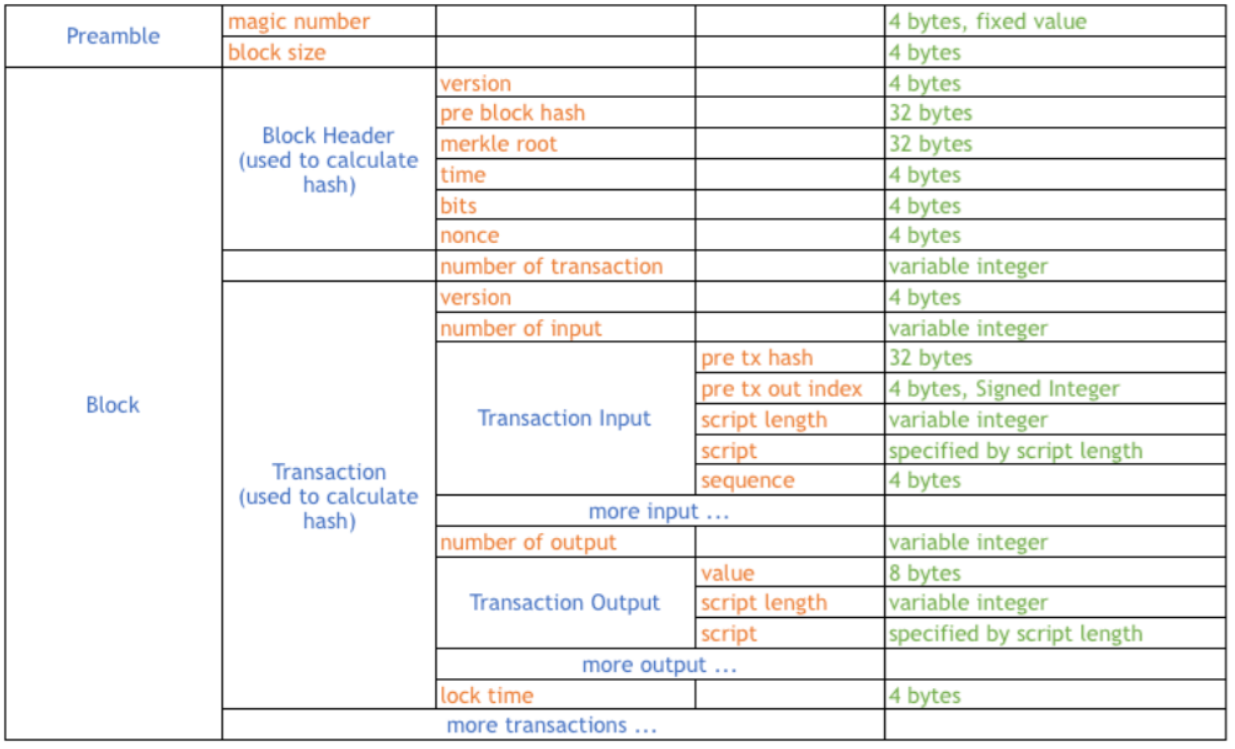
\includegraphics[width=0.9\textwidth]{./figs/block-structructure.png}
		\caption{Bitcoin's block structure~\ih{CITE https://www.blockchain.com/btc/block/100000}.}		
		\label{fig:block-structure}
	\end{center}	
\end{figure}

The block header contains several important pieces of information,
including:

\begin{itemize}
	\tightlist
	\item
	\textbf{Version}: The block version number.
	\item
	\textbf{Previous Block Hash}: The hash of the previous block's header,
	which links the blocks together in a chain.
	\item
	\textbf{Merkle Root}: The root of the Merkle tree of all the
	transactions in the block.
	\item
	\textbf{Timestamp}: The time at which the block was created.
	\item
	\textbf{Difficulty Target}: The target value that the hash of the
	block header must be less than.
	\item
	\textbf{Nonce}: A random value that is incremented by miners in the
	process of finding a valid hash.
\end{itemize}

\subsubsection{Proof-of-Work and Nakamoto's
	Consensus}\label{proof-of-work-and-nakamotos-consensus}

The security of the Bitcoin blockchain is underpinned by the
\textbf{Proof-of-Work (PoW)} consensus mechanism, often referred to as
Nakamoto's consensus. This mechanism ensures that new blocks are added
to the blockchain in a secure and decentralized manner.

In the PoW system, miners compete to solve a computationally intensive
puzzle. This puzzle involves finding a nonce that, when combined with
the other fields in the block header and hashed, produces a hash that is
below a certain target value. The first miner to find a valid hash is
rewarded with newly created bitcoins and the transaction fees from the
transactions included in the block.

The schematic diagram of finding a PoW puzzle of Bitcoin is depicted in \autoref{fig:pow-puzzle-scheme}.
\begin{figure}[t]
	%	\vspace{-0.3cm}
	\begin{center}
		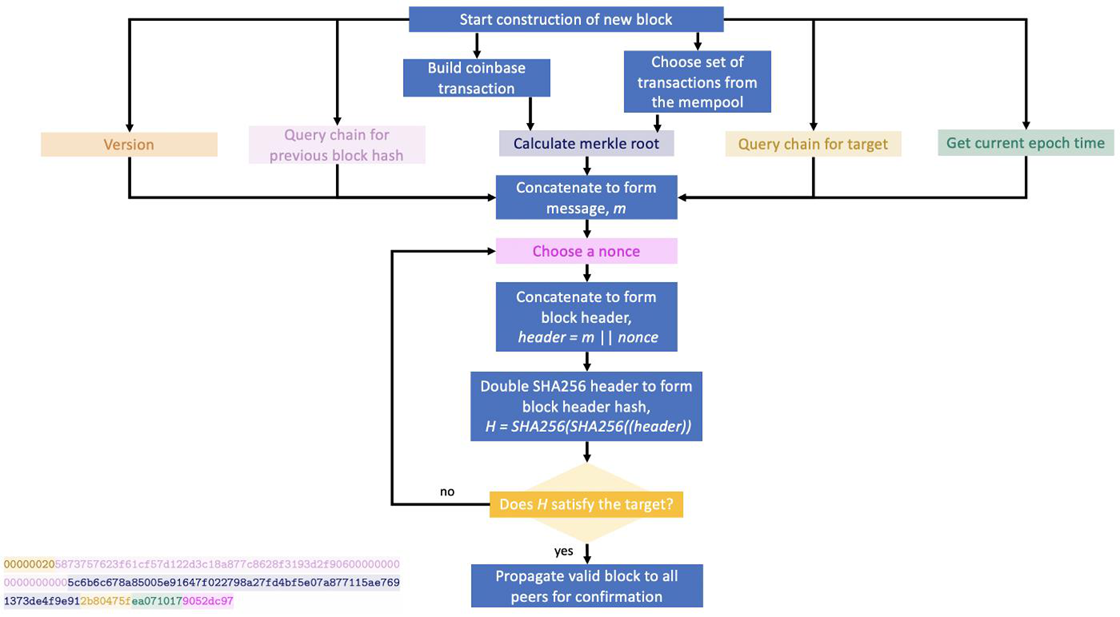
\includegraphics[width=1.1\textwidth]{./figs/pow-scheme.png}
		\caption{Finding a PoW puzzle of Bitcoin~\ih{CITE https://medium.com/fcats-blockchain-incubator/understanding-the-bitcoin-blockchain-header-a2b0db06b515}.}		
		\label{fig:pow-puzzle-scheme}
	\end{center}	
\end{figure}

Also a simplified Python code snippet that demonstrates the
Proof-of-Work algorithm is depicted in \autoref{fig:pow-puzzle-python}.
\begin{figure}[t]
	%	\vspace{-0.3cm}
	\begin{center}
		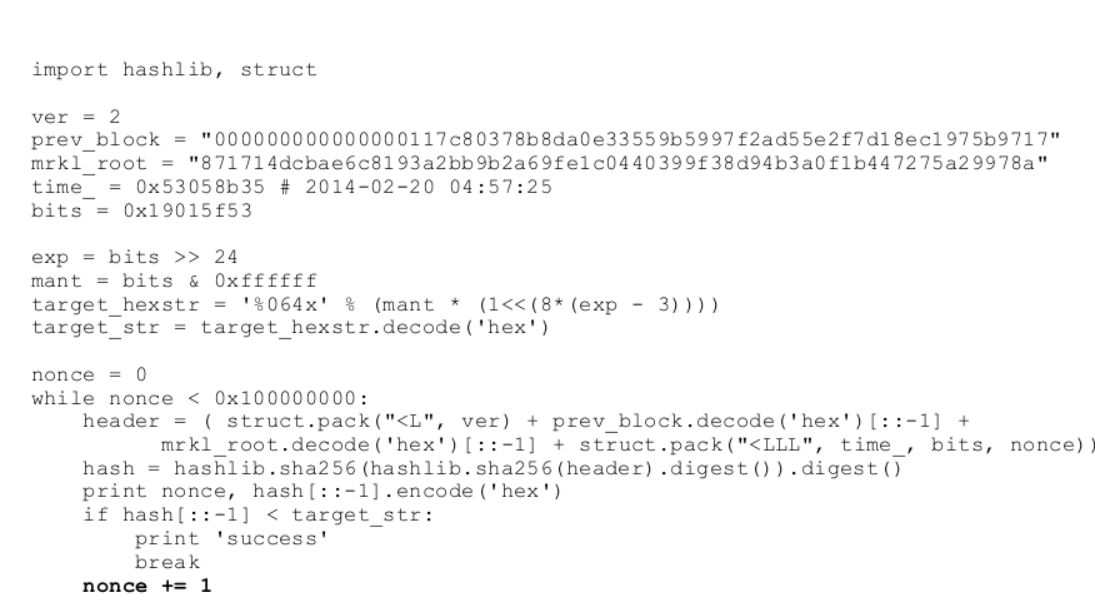
\includegraphics[width=0.9\textwidth]{./figs/pow-python.png}
		\caption{A simplified python code of finding a PoW puzzle in Bitcoin.}		
		\label{fig:pow-puzzle-python}
	\end{center}	
\end{figure}



%\begin{Shaded}
%	\begin{Highlighting}[]
%		\ImportTok{import}\NormalTok{ hashlib, struct}
%		
%		\NormalTok{ver }\OperatorTok{=} \DecValTok{2}
%		\NormalTok{prev\_block }\OperatorTok{=} \StringTok{"000000000000000117c80378b8da0e33559b5997f2ad55e2f7d18ec1975b9717"}
%		\NormalTok{mrkl\_root }\OperatorTok{=} \StringTok{"871714dcbae6c8193a2bb9b2a69fe1c0440399f38d94b3a0f1b447275a29978a"}
%		\NormalTok{time\_ }\OperatorTok{=} \BaseNTok{0x53058b35} \CommentTok{\# 2014{-}02{-}20 04:57:25}
%		\NormalTok{bits }\OperatorTok{=} \BaseNTok{0x19015f53}
%		
%		\NormalTok{exp }\OperatorTok{=}\NormalTok{ bits }\OperatorTok{\textgreater{}\textgreater{}} \DecValTok{24}
%		\NormalTok{mant }\OperatorTok{=}\NormalTok{ bits }\OperatorTok{\&} \BaseNTok{0xffffff}
%		\NormalTok{target\_hexstr }\OperatorTok{=} \StringTok{\textquotesingle{}}\SpecialCharTok{\%064x}\StringTok{\textquotesingle{}} \OperatorTok{\%}\NormalTok{ (mant }\OperatorTok{*}\NormalTok{ (}\DecValTok{1}\OperatorTok{\textless{}\textless{}}\NormalTok{(}\DecValTok{8}\OperatorTok{*}\NormalTok{(exp }\OperatorTok{{-}} \DecValTok{3}\NormalTok{))))}
%		\NormalTok{target\_str }\OperatorTok{=}\NormalTok{ target\_hexstr.decode(}\StringTok{\textquotesingle{}hex\textquotesingle{}}\NormalTok{)}
%		
%		\NormalTok{nonce }\OperatorTok{=} \DecValTok{0}
%		\ControlFlowTok{while}\NormalTok{ nonce }\OperatorTok{\textless{}} \BaseNTok{0x100000000}\NormalTok{:}
%		\NormalTok{    header }\OperatorTok{=}\NormalTok{ ( struct.pack(}\StringTok{"\textless{}L"}\NormalTok{, ver) }\OperatorTok{+}\NormalTok{ prev\_block.decode(}\StringTok{\textquotesingle{}hex\textquotesingle{}}\NormalTok{)[::}\OperatorTok{{-}}\DecValTok{1}\NormalTok{] }\OperatorTok{+}
%		\NormalTok{    mrkl\_root.decode(}\StringTok{\textquotesingle{}hex\textquotesingle{}}\NormalTok{)[::}\OperatorTok{{-}}\DecValTok{1}\NormalTok{] }\OperatorTok{+}\NormalTok{ struct.pack(}\StringTok{"\textless{}LLL"}\NormalTok{, time\_, bits, nonce))}
%		\BuiltInTok{hash} \OperatorTok{=}\NormalTok{ hashlib.sha256(hashlib.sha256(header).digest()).digest()}
%		\BuiltInTok{print}\NormalTok{ nonce, }\BuiltInTok{hash}\NormalTok{[::}\OperatorTok{{-}}\DecValTok{1}\NormalTok{].encode(}\StringTok{\textquotesingle{}hex\textquotesingle{}}\NormalTok{)}
%		\ControlFlowTok{if} \BuiltInTok{hash}\NormalTok{[::}\OperatorTok{{-}}\DecValTok{1}\NormalTok{] }\OperatorTok{\textless{}}\NormalTok{ target\_str:}
%		\BuiltInTok{print} \StringTok{\textquotesingle{}success\textquotesingle{}}
%		\ControlFlowTok{break}
%		\NormalTok{    nonce }\OperatorTok{+=} \DecValTok{1}
%	\end{Highlighting}
%\end{Shaded}

The \textbf{difficulty} of the mining puzzle is a critical parameter
that is adjusted every 2016 blocks (approximately every two weeks) to
maintain a consistent block time of around 10 minutes. If blocks are
being created too quickly, the difficulty is increased. If they are
being created too slowly, the difficulty is decreased. This ensures that
the rate of new bitcoin issuance remains predictable and that the
network remains secure.

\subsubsection{The Coinbase Transaction and the Genesis
	Block}\label{the-coinbase-transaction-and-the-genesis-block}

The first transaction in every block is a special transaction known as
the \textbf{coinbase transaction}. This transaction is created by the
miner who successfully mined the block and has two main purposes:

\begin{enumerate}
	\def\labelenumi{\arabic{enumi}.}
	\tightlist
	\item
	\textbf{Block Reward}: It allows the miner to claim the block reward,
	which is a certain number of newly created bitcoins. The block reward
	is halved approximately every four years in an event known as the
	``halving.''
	\item
	\textbf{Transaction Fees}: It allows the miner to collect the
	transaction fees from all the other transactions included in the
	block.
\end{enumerate}

The very first block in the Bitcoin blockchain, block 0, is known as the
\textbf{Genesis Block}. It was created by Satoshi Nakamoto on January 3,
2009. The coinbase transaction of the Genesis Block contains a
now-famous message: ``\textit{The Times 03/Jan/2009 Chancellor on brink of
second bailout for banks}.'' This message is widely interpreted as a
commentary on the instability of the traditional financial system and a
statement of intent for Bitcoin as a decentralized alternative.

\begin{center}\rule{0.5\linewidth}{0.5pt}\end{center}

\subsection{The UTXO Model}\label{section-4-the-utxo-model}

\subsubsection{Unspent Transaction Outputs
	(UTXOs)}\label{unspent-transaction-outputs-utxos}

Unlike traditional banking systems that use an account-based model,
Bitcoin uses the \textbf{Unspent Transaction Output (UTXO)} model to
track the ownership of funds. In the UTXO model, a user's balance is not
stored as a single value in an account. Instead, it is the sum of all
the individual, unspent transaction outputs that are locked to the
user's address.

\begin{figure}[t]
	%	\vspace{-0.3cm}
	\begin{center}
		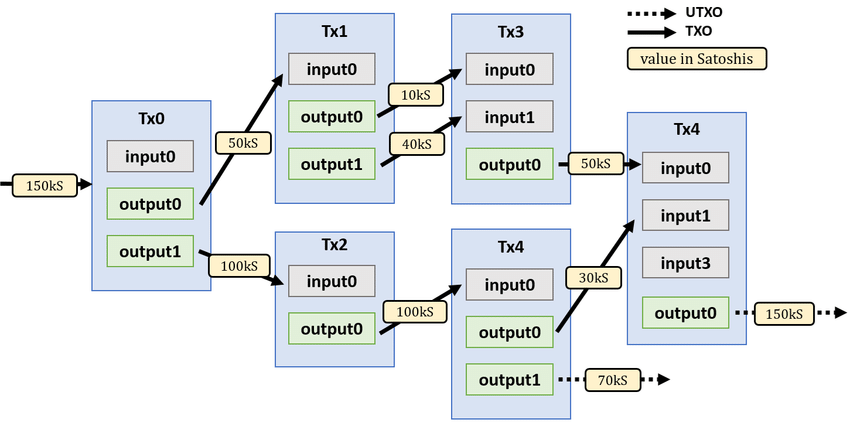
\includegraphics[width=0.9\textwidth]{./figs/utxo.png}
		\caption{Example of UTXO spending.}		
		\label{fig:utxo}
	\end{center}	
\end{figure}

A UTXO is an output of a transaction that has not yet been spent and can
be used as an input in a future transaction. Each UTXO is a discrete
amount of bitcoin that is associated with a specific address. When a
user wants to send bitcoins, their wallet selects a set of UTXOs that
are sufficient to cover the amount of the transaction. These UTXOs are
then used as inputs in the new transaction (see \autoref{fig:utxo}), and new UTXOs are created as
outputs, which are locked to the recipient's address.

Every full node in the Bitcoin network maintains a database of all the
currently unspent transaction outputs, known as the \textbf{UTXO set}. This
database is used to validate new transactions and to ensure that users
can only spend bitcoins that they actually own.

\subsubsection{Transaction Fees and Change
	Outputs}\label{transaction-fees-and-change-outputs}

\begin{itemize}
	\tightlist
	\item
	\textbf{Transaction Fees}: To incentivize miners to include their
	transactions in a block, users can include a transaction fee. The fee
	is the difference between the total value of the inputs and the total
	value of the outputs of a transaction. Miners will typically
	prioritize transactions with higher fees, as this increases their
	profitability.
	\item
	\textbf{Change Outputs}: If the total value of the UTXOs used as
	inputs in a transaction is greater than the amount the user wants to
	send, the excess amount is sent back to the user in a new UTXO, known
	as a \textbf{change output}. This is analogous to receiving change
	when paying for something with cash.
\end{itemize}

\subsubsection{Double-Spending}\label{double-spending}
Double-spending is the act of attempting to spend the same UTXO in more
than one transaction of two or more different temporary or malicious forks. The Bitcoin protocol is designed to prevent
double-spending by ensuring that only one of the conflicting
transactions can be included in the blockchain. Once a transaction is
included in a block and confirmed by the network, the UTXOs it uses as
inputs are considered spent and cannot be used again. Any subsequent
transaction that attempts to spend the same UTXOs will be rejected by
the network as invalid.

\begin{center}\rule{0.5\linewidth}{0.5pt}\end{center}

\subsection{The Lightning Network: A Scalability
	Solution}\label{section-5-the-lightning-network-a-scalability-solution}

One of the most significant challenges facing Bitcoin is its limited
scalability. The combination of a 4 MB block size limit and a 10-minute block time restricts the network's
transaction throughput to approximately 7 transactions per second. This
is a major bottleneck that prevents Bitcoin from being used as a global
payment system for everyday transactions, which would require a much
higher throughput.

\subsubsection{The Lightning Network}\label{the-lightning-network}

The Lightning Network is a Layer 2 scaling solution that is designed to
address Bitcoin's scalability limitations. It is a decentralized network
of off-chain payment channels that allows for instant, low-cost
transactions.

The core idea behind the Lightning Network is to move the majority of
transactions off the main Bitcoin blockchain. Users can open payment
channels with each other by committing a certain amount of bitcoin to a
multi-signature address. Once a channel is open, the two parties can
transact with each other an unlimited number of times without having to
broadcast each transaction to the main blockchain. In this way pairwise network is formed and LN transactions can be route through intermediaries that have sufficient channel capacity (see \autoref{fig:ln}) -- in turn these intermediaries earn routing fees. This allows for instant and virtually free transactions.

\begin{figure}[t]
	%	\vspace{-0.3cm}
	\begin{center}
		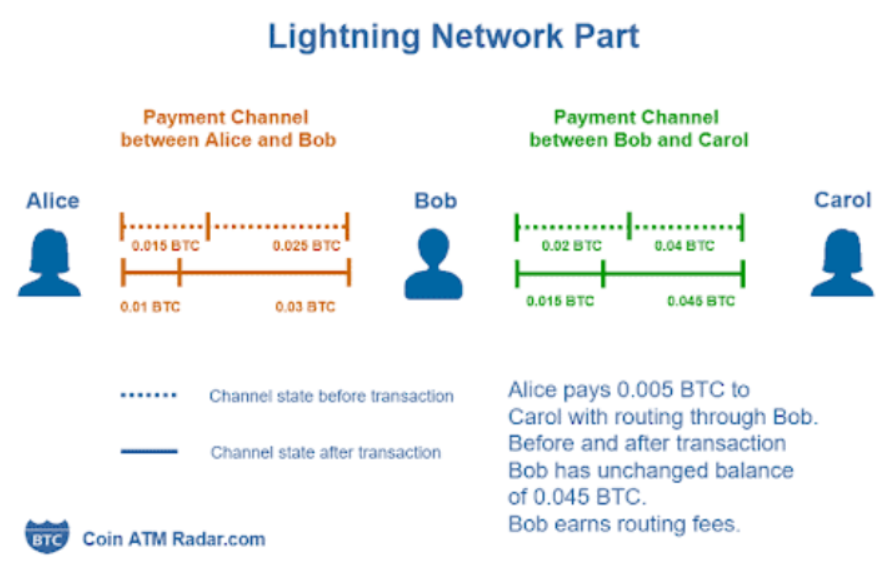
\includegraphics[width=0.9\textwidth]{./figs/ln.png}
		\caption{Lightning network routing and channel update (i.e., balance change).}		
		\label{fig:ln}
	\end{center}	
\end{figure}

The main blockchain is only used to open and close the payment channels.
When the two parties decide to close the channel, the final balance is
settled on the Bitcoin blockchain.

The Lightning Network uses a clever mechanism called \textbf{Hashed
	Time-Locked Contracts (HTLCs)} to enable trustless, multi-hop payments
across the network. This means that two users can transact with each
other even if they do not have a direct payment channel, as long as
there is a path of connected channels between them. In particular, hash time locks enable to conditionally redeem funds by recipient from the sender's output if the pre-image of a hash is revealed in specified time windows. If it is not revealed the funds can be redeemed back by the sender.

\begin{center}\rule{0.5\linewidth}{0.5pt}\end{center}

\subsection{Summary / Key Takeaways}\label{summary-key-takeaways}

This section has provided a detailed introduction to the world of
Bitcoin, the first and most prominent cryptocurrency. We have explored
its origins in the context of the 2008 financial crisis, its core
principles of decentralization and censorship resistance, and the key
technological components that make it function.

We have delved into the peer-to-peer architecture of the Bitcoin
network, identifying the various roles of its participants, from clients
and full nodes to miners. We have also examined the structure of Bitcoin
transactions and blocks, and the crucial role of the Merkle tree in
ensuring data integrity.

A key focus of this section has been the UTXO model, which is Bitcoin's
unique approach to tracking the ownership of funds. We have also
explored the Proof-of-Work consensus mechanism, which is the engine that
secures the Bitcoin blockchain and ensures its immutability.

Finally, we have acknowledged the challenges that Bitcoin faces,
particularly in the areas of scalability and privacy, and we have
introduced the Lightning Network as a promising Layer 2 solution that
aims to address these challenges. This section has laid the groundwork
for a deeper understanding of more advanced topics in blockchain
technology and decentralized applications.

\begin{center}\rule{0.5\linewidth}{0.5pt}\end{center}

\subsection{Keywords}\label{keywords}

\begin{itemize}
	\tightlist
	\item
	\textbf{Bitcoin}: A decentralized digital currency that enables
	peer-to-peer transactions without the need for a central authority.
	\item
	\textbf{Proof-of-Work (PoW)}: A consensus mechanism that secures a
	blockchain by requiring participants to solve a computationally
	intensive puzzle.
	\item
	\textbf{UTXO (Unspent Transaction Output)}: The fundamental building
	block of a Bitcoin transaction, representing a discrete amount of
	bitcoin that can be spent.
	\item
	\textbf{Mining}: The process of creating new blocks in a Proof-of-Work
	blockchain by solving the computational puzzle.
	\item
	\textbf{Lightning Network}: A Layer 2 payment protocol that operates
	on top of the Bitcoin blockchain, enabling fast and low-cost
	transactions.
	\item
	\textbf{Satoshi Nakamoto}: The pseudonymous creator of Bitcoin.
	\item
	\textbf{Genesis Block}: The first block in the Bitcoin blockchain.
	\item
	\textbf{Coinbase Transaction}: A special transaction in each block
	that rewards the miner with newly created bitcoins and transaction
	fees.
	\item
	\textbf{Double-Spending}: The act of spending the same UTXO in
	multiple transactions.
	\item
	\textbf{Hashed Time-Locked Contract (HTLC)}: A type of smart contract
	used in the Lightning Network to enable trustless, multi-hop payments.
\end{itemize}

\begin{center}\rule{0.5\linewidth}{0.5pt}\end{center}

\subsection{Further Reading}\label{further-reading}

\begin{itemize}
	\tightlist
	\item
	\textbf{Bitcoin: A Peer-to-Peer Electronic Cash System}:\\
	\url{https://bitcoin.org/bitcoin.pdf}
	\item
	\textbf{Bitcoin Developer Guide}:\\
	\url{https://bitcoin.org/en/developer-guide}
	\item
	\textbf{Mastering Bitcoin by Andreas M. Antonopoulos}:\\
	\url{https://github.com/bitcoinbook/bitcoinbook}
\end{itemize}

\newpage

\section{Bitcoin (Part II)}\label{chapter-3-bitcoin-part-2}
Building upon the foundational concepts introduced in the previous
section, this section delves deeper into the technical intricacies of
the Bitcoin protocol. We will begin by exploring Bitcoin Script, the
simple yet powerful scripting language that underpins all Bitcoin
transactions. We will examine how this stack-based language is used to
create sophisticated spending conditions, enabling a wide range of
transaction types beyond simple payments.

The section will then trace the evolution of Bitcoin's standard script
types, from the early Pay-to-Public-Key (P2PK) and
Pay-to-Public-Key-Hash (P2PKH) scripts to the more advanced
Pay-to-Script-Hash (P2SH) and multi-signature (P2MS) scripts. We will
analyze the motivation behind each of these developments and the new
capabilities they introduced.

A significant portion of this section is dedicated to the two most
important upgrades in Bitcoin's history: Segregated Witness (SegWit) and
Taproot. We will explore the technical details of these upgrades,
including how SegWit solved the long-standing problem of transaction
malleability and how Taproot introduced Schnorr signatures and
Merkelized Alternative Script Trees (MAST) to enhance privacy,
efficiency, and smart contract capabilities.

%\ih{drop} Finally, we will discuss the concept of blockchain forks in greater
%detail, examining the different types of forks and their implications
%for the network. We will also analyze the threat of a 51\% attack and
%other potential vulnerabilities that could compromise the security and
%integrity of the Bitcoin network.

\subsection{Learning Objectives}\label{learning-objectives}

\begin{itemize}
	\tightlist
	\item
	Understand the fundamentals of Bitcoin Script and its role in defining
	spending conditions.
	\item
	Learn about the different standard script types, including P2PK,
	P2PKH, P2SH, and the various SegWit and Taproot formats.
	\item
	Grasp the concepts of transaction malleability and how Segregated
	Witness (SegWit) addresses this issue.
	\item
	Understand the benefits of the Taproot upgrade, including improved
	privacy and efficiency.
%	\item
%	\ih{drop} Learn about the different types of blockchain forks and their
%	implications for the network.
	\item
	Gain insight into the 51\% attack and other potential vulnerabilities
	in the Bitcoin network.
\end{itemize}

\begin{center}\rule{0.5\linewidth}{0.5pt}\end{center}

\subsection{The UTXO Model and Bitcoin
	Script}\label{section-1-the-utxo-model-and-bitcoin-script}

\subsubsection{Recap of the UTXO
	Model}\label{recap-of-the-utxo-model}

As established in the preceding section, the Bitcoin protocol employs
the \textbf{Unspent Transaction Output (UTXO)} model as its fundamental
accounting mechanism. This model represents a paradigm shift from the
traditional account-based systems used in conventional finance. Instead
of maintaining balances in accounts, the Bitcoin ledger comprises a
collection of UTXOs, each representing a discrete and unspent amount of
bitcoins. Every transaction consumes one or more UTXOs as inputs and
generates one or more new UTXOs as outputs, thereby creating a
continuous and verifiable chain of ownership.

\subsubsection{Introduction to Bitcoin
	Script}\label{introduction-to-bitcoin-script}

At the heart of the UTXO model is \textbf{Bitcoin Script}, a simple,
stack-based programming language that governs the spending conditions
for each UTXO. Every transaction output is encumbered with a locking
script, formally known as \texttt{ScriptPubKey}, which specifies the
conditions that must be met to spend the associated funds. To redeem a
UTXO, a subsequent transaction must provide a corresponding unlocking
script, or \texttt{ScriptSig}, that satisfies the requirements of the
\texttt{ScriptPubKey} (see \autoref{fig:utxo-unlock}).


\begin{figure}[t]
	%	\vspace{-0.3cm}
	\begin{center}
		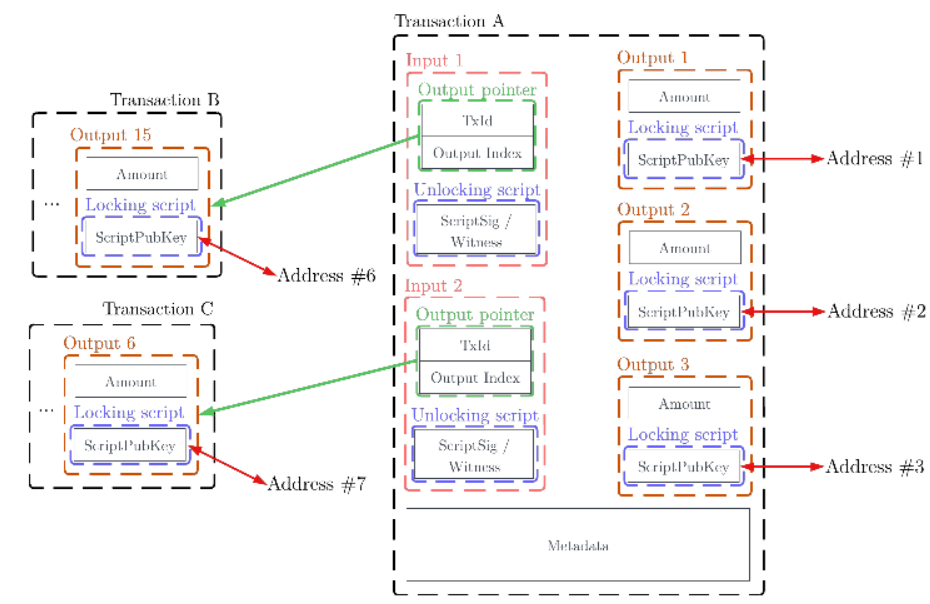
\includegraphics[width=0.9\textwidth]{./figs/utxo-unlocking.png}
		\caption{Bitcoin transaction with locking and unlocking scripts.}		
		\label{fig:utxo-unlock}
	\end{center}	
\end{figure}



The design of Bitcoin Script is intentionally minimalistic. It is not
Turing-complete, meaning that it lacks the ability to perform loops or
complex recursive operations. This limitation is a deliberate security
feature, designed to prevent the execution of overly complex or
malicious scripts that could potentially disrupt the network.

\subsubsection{Standard Script Types}\label{standard-script-types}

While Bitcoin Script allows for a high degree of flexibility in defining
spending conditions, a set of standard script types has emerged over
time to accommodate the most common use cases. These standard scripts
are recognized and relayed by all nodes in the network, ensuring a high
degree of interoperability.

\begin{itemize}
	\item
	\textbf{Pay-to-Public-Key (P2PK)}: This was the original script type
	used in the earliest days of Bitcoin. It locks a UTXO directly to a
	specific public key, and the corresponding unlocking script simply
	requires a valid signature from the owner of that public key. While
	simple, P2PK has been largely superseded by more advanced script
	types.
	\item
	\textbf{Pay-to-Public-Key-Hash (P2PKH)}: This is the most common
	script type in use today. Instead of locking a UTXO to a public key,
	it locks it to the hash of a public key. This provides two main
	advantages: it results in a shorter and more convenient address
	format, and it offers a degree of privacy protection, as the public key is not revealed until the UTXO is spent.
	\item
	\textbf{Pay-to-MultiSig (P2MS)}: This script type enables
	multi-signature transactions, which require the approval of multiple
	parties to spend a UTXO. A P2MS script specifies a set of \texttt{n}
	public keys and a threshold \texttt{m}, where
	$m \leq n$. To spend the UTXO, at least \texttt{m}
	valid signatures corresponding to the specified public keys must be
	provided.
	\item
	\textbf{Pay-to-Script-Hash (P2SH)}: This is a more advanced and
	flexible script type that allows a UTXO to be locked to the hash of an
	arbitrary script. This enables the creation of complex spending
	conditions without revealing the underlying script until the UTXO is
	spent. P2SH is commonly used for multi-signature wallets and other
	advanced smart contract-like functionality.
\end{itemize}

\begin{center}\rule{0.5\linewidth}{0.5pt}\end{center}

\subsection{Segregated Witness (SegWit) and
	Taproot}\label{section-2-segregated-witness-segwit-and-taproot}

\subsubsection{The Need for Upgrades}\label{the-need-for-upgrades}

As the Bitcoin network grew and evolved, several limitations of the
original protocol became apparent: 

\begin{itemize}
	\tightlist
	\item
	\textbf{Transaction Malleability}: This was a long-standing
	vulnerability in the Bitcoin protocol that allowed a third party to
	alter the signature data of an unconfirmed transaction, thereby
	changing its transaction ID (TXID) without invalidating the
	transaction itself. This could cause problems for services that relied
	on unconfirmed transactions, such as payment processors and exchanges. \ih{check it}
	\item
	\textbf{Scalability}: The 1 MB block size limit severely restricted
	the number of transactions that could be processed by the network,
	leading to congestion and high fees during periods of high demand.
	\item
	\textbf{Privacy}: The public nature of the blockchain made it possible
	to analyze transaction patterns and link addresses to real-world
	identities, raising privacy concerns for users.
\end{itemize}
These challenges prompted the
development of two major upgrades: Segregated Witness (SegWit) and
Taproot \ih{refs on BIPs}. 

\subsubsection{Segregated Witness
	(SegWit)}\label{segregated-witness-segwit}

Segregated Witness (SegWit) was a soft fork upgrade that was activated
on the Bitcoin network in August 2017. It addressed the issue of
transaction malleability by separating the \textbf{signature data}, or
``\textbf{witness},'' from the main transaction data. By moving the witness data to a separate data structure, SegWit made it impossible for a third
party to alter the signature and change the TXID.

In addition to fixing transaction malleability, SegWit also introduced a
new concept of ``block weight,'' which effectively increased the block
size limit to 4 MB for blocks containing SegWit transactions. This
allowed for more transactions to be included in each block, thereby
improving the scalability of the network.

SegWit also introduced new address formats, known as \textbf{P2WPKH
(Pay-to-Witness-Public-Key-Hash)} and \textbf{P2WSH (Pay-to-Witness-Script-Hash)},
which offer lower transaction fees than their legacy counterparts. To
ensure backward compatibility, SegWit also provided a mechanism for
``wrapping'' SegWit transactions in P2SH addresses.
Overview of all existing output types in UTXO is depicted in \autoref{fig:btc-scripts}.

\begin{table}[t]
	%	\vspace{-0.3cm}
	\begin{center}
		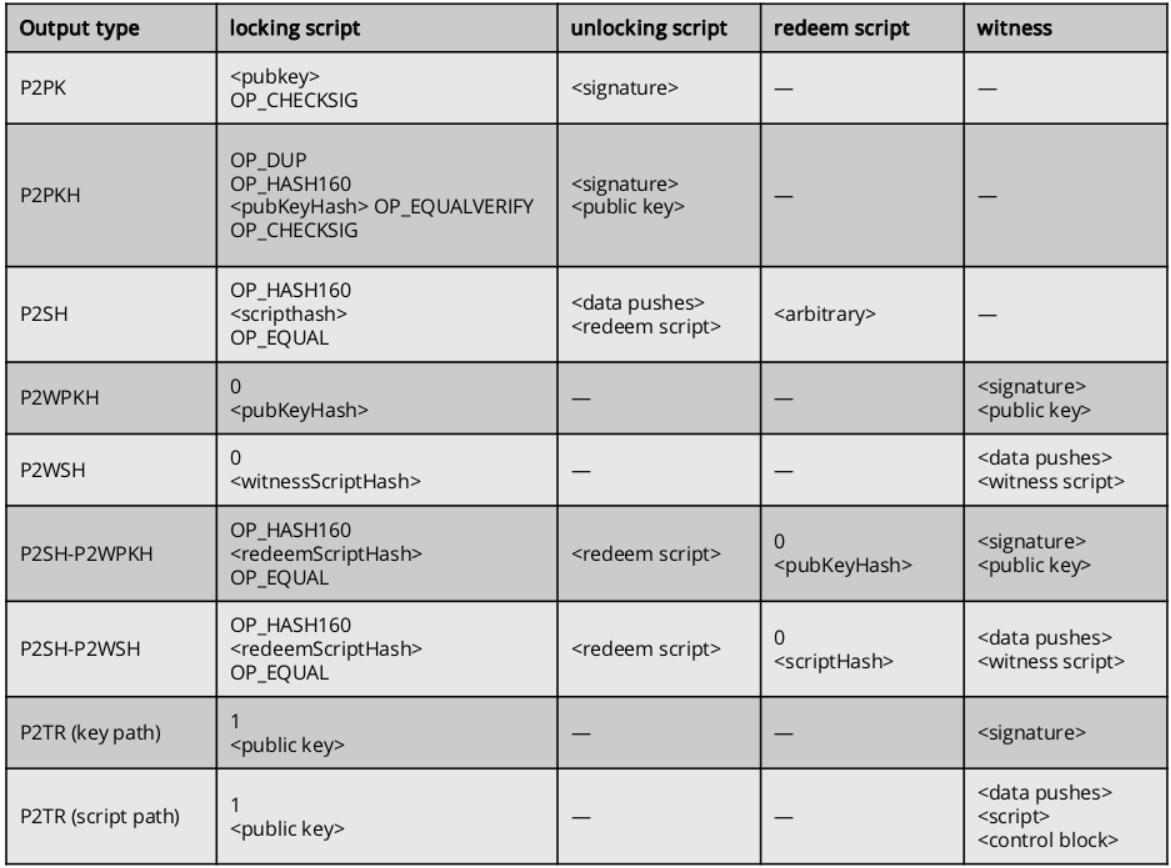
\includegraphics[width=0.9\textwidth]{./figs/scripts}
		\caption{Output types in UTXO and their locking and unlocking scripts.}		
		\label{fig:btc-scripts}
	\end{center}	
\end{table}

\subsubsection{Taproot}\label{taproot}

Taproot is the most significant upgrade to the Bitcoin protocol since
SegWit, and it was activated in November 2021. It introduced a number of
new features that further enhance the privacy, efficiency, and smart
contract capabilities of the network. I  particular, Taproot introduced the following:

\begin{itemize}
	\item
	\textbf{Schnorr Signatures}: Taproot replaced the Elliptic Curve
	Digital Signature Algorithm (ECDSA) with Schnorr signatures. Schnorr
	signatures offer several advantages over ECDSA, including their
	smaller size and their ability to be aggregated. This means that
	multiple signatures can be combined into a single signature, which
	makes multi-signature transactions indistinguishable from
	single-signature transactions on the blockchain. This significantly
	improves the privacy of multi-signature wallets and reduces their
	transaction fees since only one signature is enough to be stored.
	\item
	\textbf{MAST (Merkelized Alternative Script Trees)}: Taproot also
	introduced Merkelized Alternative Script Trees (MAST), a new way of
	constructing complex spending conditions. With MAST, a user can create
	a tree of different scripts, each representing a different spending
	condition. When the UTXO is spent, only the script that is actually
	used is revealed on the blockchain. This improves privacy by hiding
	the other possible spending conditions, and it also reduces the amount
	of data that needs to be stored on the blockchain, thereby improving
	efficiency.
\end{itemize}

\subsubsection{Ordinals and
	Inscriptions}\label{ordinals-and-inscriptions}

The Taproot upgrade had an unforeseen consequence: the emergence of
\textbf{Ordinals and Inscriptions}. The Ordinals protocol is a system
for numbering individual satoshis\ih{check this}, the smallest unit of bitcoin, and
tracking them across transactions. The Inscriptions protocol allows
users to inscribe arbitrary data, such as images and text, onto
individual satoshis.

This has led to the creation of NFT-like assets on the Bitcoin
blockchain, which has been a source of considerable controversy within
the community. While some see it as an innovative new use case for
Bitcoin, others are concerned that it is leading to network congestion
and higher transaction fees, and that it is a departure from Bitcoin's
original purpose as a peer-to-peer electronic cash system.

\begin{center}\rule{0.5\linewidth}{0.5pt}\end{center}

\subsection{The 51\% Attack}\label{section-3-blockchain-forks-and-network-security}

A 51\% attack is a potential attack on a Proof-of-Work blockchain where
a single entity or a group of colluding entities gains control of more
than 50\% of the network's total mining hash rate. With this level of
control, an attacker could theoretically:

\begin{itemize}
	\tightlist
	\item
	\textbf{Prevent new transactions from being confirmed}: By refusing to
	include certain transactions in the blocks they mine, an attacker
	could effectively censor users.
	\item
	\textbf{Halt payments between some or all users}: By creating empty
	blocks, an attacker could prevent any transactions from being
	processed.
	\item
	\textbf{Reverse transactions}: An attacker could use their majority
	hash power to create a private chain that is longer than the public
	chain. They could then broadcast this longer chain to the network,
	which would cause the public chain to be orphaned and all the
	transactions in it to be reversed. This would allow the attacker to
	double-spend their coins.
\end{itemize}

While a 51\% attack is a serious threat, it is important to note that it
is extremely difficult and expensive to execute on a large and
decentralized network like Bitcoin. The cost of acquiring the necessary
hardware and electricity to control more than 50\% of the Bitcoin
network's hash rate would be astronomical. Furthermore, a successful
51\% attack would likely undermine confidence in the network, causing
the price of the cryptocurrency to plummet and rendering the attack
unprofitable.

\begin{center}\rule{0.5\linewidth}{0.5pt}\end{center}

\subsection{Summary / Key Takeaways}\label{summary-key-takeaways}

This section has provided a deep dive into the advanced technical
aspects of the Bitcoin protocol, building upon the foundational
knowledge from the previous section. We have explored the evolution of
Bitcoin's scripting capabilities, from the simple yet powerful Bitcoin
Script to the sophisticated features introduced by the SegWit and
Taproot upgrades.

We have examined the various standard script types, including P2PK,
P2PKH, P2MS, and P2SH, and we have seen how they enable a wide range of
transaction types. We have also analyzed the motivations behind the
SegWit and Taproot upgrades, and we have seen how they have addressed
key challenges such as transaction malleability, scalability, and
privacy.

\begin{center}\rule{0.5\linewidth}{0.5pt}\end{center}

\subsection{Keywords}\label{keywords}

\begin{itemize}
	\tightlist
	\item
	\textbf{Bitcoin Script}: A simple, stack-based programming language
	that is used to define the conditions under which a UTXO can be spent.
	\item
	\textbf{Segregated Witness (SegWit)}: A protocol upgrade that
	addresses transaction malleability and increases the effective block
	size by separating the signature data from the main transaction data.
	\item
	\textbf{Taproot}: A protocol upgrade that enhances privacy,
	efficiency, and smart contract capabilities through the introduction
	of Schnorr signatures and Merkelized Alternative Script Trees (MAST).
	\item
	\textbf{Blockchain Fork}: A divergence in the blockchain that results
	in two or more competing chains.
	\item
	\textbf{51\% Attack}: A potential attack on a Proof-of-Work blockchain
	where a single entity controls more than 50\% of the network's mining
	hash rate.
	\item
	\textbf{P2PKH (Pay-to-Public-Key-Hash)}: The most common type of
	Bitcoin transaction, where the output is locked to the hash of a
	public key.
	\item
	\textbf{P2SH (Pay-to-Script-Hash)}: A type of Bitcoin transaction that
	allows for more complex spending conditions by locking the output to
	the hash of a script.
	\item
	\textbf{Schnorr Signatures}: A digital signature scheme that is more
	efficient and secure than ECDSA and allows for key and signature
	aggregation.
	\item
	\textbf{MAST (Merkelized Alternative Script Trees)}: A mechanism that
	allows for more complex and flexible smart contracts by enabling the
	creation of a tree of possible spending conditions.
	\item
	\textbf{Ordinals and Inscriptions}: A protocol that allows for the
	creation of NFT-like assets on the Bitcoin blockchain.
\end{itemize}

\begin{center}\rule{0.5\linewidth}{0.5pt}\end{center}

\subsection{Further Reading}\label{further-reading}

\begin{itemize}
	\tightlist
	\item
	\textbf{Bitcoin Improvement Proposals (BIPs)}:\\
	\url{https://github.com/bitcoin/bips}
	\item
	\textbf{Learn Me a Bitcoin}: \\ 
	\url{https://learnmeabitcoin.com/}
	\item
	\textbf{Mempool.space}: \\
	\url{https://mempool.space/}
\end{itemize}
\newpage

\section{Ethereum v1.0 (PoW) and Smart Contracts}\label{chapter-4-Eth1}
This section provides a comprehensive introduction to Ethereum v1.0, a
decentralized, open-source blockchain platform that has revolutionized
the field of distributed computing. While Bitcoin introduced the world
to the concept of a peer-to-peer electronic cash system, Ethereum
expanded on this vision by creating a general-purpose blockchain that
enables developers to build and deploy a wide range of decentralized
applications (DAPPs) and smart contracts.

We will begin by exploring the historical context and motivation behind
the creation of Ethereum, including the limitations of Bitcoin's
scripting language that inspired Vitalik Buterin and Gavin Wood to propose a more
flexible and expressive platform. We will then delve into the core
concepts that define the Ethereum ecosystem, such as the Ethereum
Virtual Machine (EVM), the account-based model, and the concept of gas,
which is used to meter the computational resources of the network.

A significant portion of this section will be dedicated to understanding
the technical underpinnings of Ethereum, including the structure of
transactions and blocks, and the use of Merkle-Patricia trees to
efficiently store and verify the global state of the network. By the end
of this section, you will have a solid understanding of the fundamental
principles of Ethereum and the key technological innovations that have
made it the leading platform for smart contracts and decentralized
applications.

\subsection{Learning Objectives}\label{learning-objectives}

\begin{itemize}
	\tightlist
	\item
	Understand the concept of smart contracts and their potential
	applications.
	\item
	Learn about the history and motivation behind the creation of
	Ethereum.
	\item
	Grasp the key features of the Ethereum platform, including its
	Turing-complete scripting language and the Ethereum Virtual Machine
	(EVM).
	\item
	Understand the Ethereum account model and how it differs from
	Bitcoin's UTXO model.
	\item
	Learn about the concept of gas and its role in preventing abuse of the
	network.
	\item
	Gain insight into the structure of Ethereum transactions and blocks.
	\item
	Understand the purpose and function of the Merkle-Patricia Tree in
	managing Ethereum's global state.
\end{itemize}

\begin{center}\rule{0.5\linewidth}{0.5pt}\end{center}

\subsection{The Motivation for Smart
	Contracts}\label{section-1-the-motivation-for-smart-contracts}

\subsubsection{From Legal Contracts to Smart
	Contracts}\label{from-legal-contracts-to-smart-contracts}

Traditional legal contracts, while a cornerstone of modern commerce, are
often fraught with inefficiencies. They can be slow to draft, expensive
to enforce, and subject to the ambiguities of human language. In 1994,
long before the advent of blockchain technology, computer scientist and
cryptographer Nick Szabo envisioned a more efficient and secure
alternative: the \textbf{smart contract}.

Szabo defined a smart contract as a computerized transaction protocol
that executes the terms of a contract. The primary objectives of this
concept were to:

\begin{itemize}
	\tightlist
	\item
	\textbf{Automate Contractual Obligations}: To automatically enforce
	the terms of an agreement, such as payment terms, without the need for
	manual intervention.
	\item
	\textbf{Minimize Exceptions}: To reduce the risk of both malicious and
	accidental exceptions by encoding the terms of the contract in a
	deterministic and unambiguous programming language.
	\item
	\textbf{Reduce Reliance on Trusted Intermediaries}: To minimize the
	need for trusted third parties, such as lawyers and escrow agents,
	thereby reducing transaction costs and increasing efficiency.
\end{itemize}

%A classic example illustrating the need for such automation is an
%\textbf{escrow} service. When buying a house, a significant problem is
%determining the order of operations: should the buyer pay first, or
%should the seller transfer the property title first? An escrow service,
%a trusted third party, solves this by holding the buyer's funds until
%the title transfer is complete. Smart contracts aim to replace such
%intermediaries with automated, trustless code.

\subsubsection{The Limitations of Bitcoin
	Script}\label{the-limitations-of-bitcoin-script}

The Bitcoin protocol, with its simple, stack-based scripting language,
provided the first glimpse of the potential of smart contracts. Bitcoin
Script allows for the creation of basic spending conditions, such as
multi-signature transactions and time-locked payments. However, the
language is intentionally limited in its functionality -- it is not
Turing-complete -- to prioritize security and prevent complex,
potentially malicious scripts from being executed on the network. However, a simple stack-based automaton is insufficient
for Turing-completeness; a more powerful mechanism is required.

This limitation, while a sensible design choice for a digital currency,
made it difficult to build more complex and sophisticated applications
on top of the Bitcoin blockchain. The need for a more general-purpose
blockchain platform with a Turing-complete scripting language was the
primary motivation for the creation of Ethereum.

\begin{center}\rule{0.5\linewidth}{0.5pt}\end{center}

\subsection{An Introduction to
	Ethereum}\label{section-2-an-introduction-to-ethereum}

\subsubsection{The Vision of a World
	Computer}\label{the-vision-of-a-world-computer}

Launched in 2015, Ethereum was conceived with the ambitious vision of
creating a ``world computer'' -- a single, decentralized platform capable
of running any application. This vision was a direct response to the
limitations of Bitcoin, which, while revolutionary, was primarily
designed as a peer-to-peer electronic cash system. Ethereum, in
contrast, was designed to be a general-purpose blockchain, providing
developers with the tools and flexibility to build and deploy their own
smart contracts and decentralized applications (DAPPs).
The key features that enable this vision include:

\begin{itemize}
	\tightlist
	\item
	\textbf{Quasi-Turing-complete Smart Contracts}: Ethereum's primary
	programming language, Solidity, is often described as Turing-complete,
	meaning it can compute anything that is computable. However, this is
	practically limited by the concept of ``gas'' to prevent infinite
	loops. This allows for the creation of sophisticated DAPPs that can
	automate a wide range of processes and interactions.
	\item
	\textbf{The Ethereum Virtual Machine (EVM)}: The EVM is the runtime
	environment for smart contracts on the Ethereum network. It is a
	sandboxed virtual machine that is completely isolated from the host
	node's network, filesystem, or processes, ensuring that smart
	contracts are executed in a secure and deterministic manner.
	\item
	\textbf{Decentralized Finance (DeFi)}: Ethereum's flexible and
	expressive smart contract capabilities have made it the leading
	platform for the burgeoning field of Decentralized Finance (DeFi).
	DeFi applications aim to recreate traditional financial services, such
	as lending, borrowing, and trading, in a decentralized and
	permissionless manner.
\end{itemize}

\subsubsection{The Ethereum Account
	Model}\label{the-ethereum-account-model}

A key architectural difference between Bitcoin and Ethereum is their
respective account models. While Bitcoin uses the \textbf{Unspent
	Transaction Output (UTXO)} model, Ethereum employs an
\textbf{account-balance-based model}, which is more analogous to a traditional
bank account. There are two types of accounts in Ethereum:

\begin{itemize}
	\tightlist
	\item
	\textbf{Externally Owned Accounts (EOAs)}: These accounts are
	controlled by users via their private keys. EOAs can send transactions
	to other accounts and can trigger the execution of smart contracts.
	\item
	\textbf{Contract Accounts}: These accounts are controlled by the code
	of a smart contract. A contract account is created when a smart
	contract is deployed to the blockchain, and it can only execute code
	in response to a transaction or a message call from another account.
\end{itemize}

Each Ethereum account is associated with a unique 20B-long address and maintains
a state that includes its balance of Ether (ETH), the native
cryptocurrency of the Ethereum network, as well as a \textbf{nonce} (a
transaction counter to prevent replay attacks), a \textbf{storage root},
and a \textbf{code hash}.
Nonce field has context-based interpretation and based on the account type.
In the case of EOA account, the value of nonce represents the number of transactions sent from this account while in the case of smart contract account, the nonce value represents the number of smart contract creations made by tbe smart contract account.
Note that the code hash stands for the cryptographically hashed EVM bytecode of the smart contract account, while the code fragments are stored in a dedicated state database, under their hashes -- this is to efficiently optimize the storage for the same codes. The code hash field is immutable (unlike other fields).

\subsubsection{The concept of Gas}\label{gas-and-the-ethereum-virtual-machine-evm}

To prevent the network from being bogged down by infinite loops or other
forms of computational abuse, Ethereum incorporates a mechanism known as
\textbf{gas}. Gas is a unit of measurement for the computational effort
required to execute operations on the EVM. Every operation, from a
simple addition to a complex storage write, has a specific gas cost.

When a user sends a transaction, they must specify a \textbf{gas limit},
which is the maximum amount of gas they are willing to pay for the
transaction. They must also specify a \textbf{gas price}, which is the
amount of Ether they are willing to pay per unit of gas. The total cost
of the transaction is the product of the gas used and the gas price.
This system ensures that the network's computational resources are
allocated efficiently and provides a mechanism for compensating miners
for their work. If a transaction runs out of gas, its operations are
reverted, but the fee is still paid to the miner.

The EVM itself is a stack-based virtual machine with a 256-bit word
size. It provides a secure and deterministic environment for executing
smart contracts, ensuring that all nodes in the network will arrive at
the same result when executing the same code.

\paragraph{\textbf{Gas Price.}}
Every instruction of the EVM has a different gas price, mostly depending on whether it modifies storage or works only with memory. 
In general, the operations with volatile memory are cheap while permanent modification to storage are expensive.
See the example of gas prices of various instructions in \autoref{fig:eth-gas-price}, as introduced by the original version of the Ethereum Yellow paper~\cite{wood2014ethereum}. Note that the transfer transactions costs 21k of gas, which is often used as a baseline for comparison with other smart contract calls.


\begin{figure}[t]
	%	\vspace{-0.3cm}
	\begin{center}
		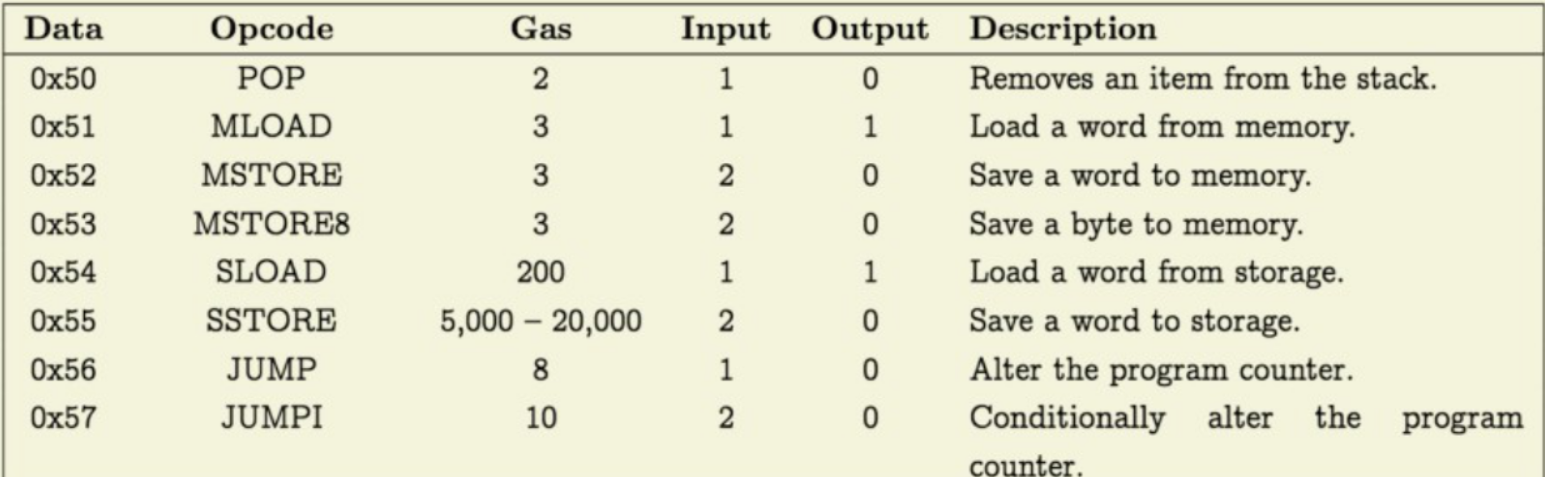
\includegraphics[width=0.9\textwidth]{./figs/gas-price.png}
		\caption{Gas prices of some EVM instructions.}		
		\label{fig:eth-gas-price}
	\end{center}	
\end{figure}

\paragraph{\textbf{Execution of Transaction Calling Smart Contract.}}
The simple pseudocode of deducting gas while doing transaction execution in EVM is described in the following listing:
\begin{enumerate}
	\tightlist
	\item Specify startGas and gasPrice
	\item  Assert(startGas*gasPrice $\leq$ balanceOfCaller)
	\item  balanceOfCaller -= startGas*gasPrice
	\item tmpGas = startGas ; gasRefund = 0
	\item Execute code, deducting from tmpGas
	\begin{itemize}
		\item deducted = ExecutionCost(tx)
		\item \textbf{If} deducted $<$ 0 \textbf{then} \\
		\hspace{0.5cm} ~~~~gasRefund += $|$deducted$|$ \\
		\textbf{else} \\
		\hspace{0.5cm} ~~~~tmpGas -= deducted \\
		\item Assert(tmpGas$\geq$ 0)
	\end{itemize}
	
	\item Refund gasRefund + tmpGas to balanceOfCaller	
\end{enumerate}



\subsubsection{EIP-1559}\label{gas-and-the-ethereum-virtual-machine-evm}
The EIPT-1559 \ih{ref} was included in London's hardfork that occurred on 5th of August 2021, and its main contribution is to optimize the fee market system.
In particular, this EIP introduces 3 elements of gas:
\begin{itemize}
	\item \textbf{Base fee} -- the minimum amount of gas for a transaction, which is burnt. It is set by the network. Blocks can be extended to 200\% of the base fee.
	
	\item \textbf{Tip} -- is set by the user, and it represents a premium to miners that should prioritize the faster inclusion of their transaction.
	
	\item \textbf{Fee cap} -- represents the the maximum amount of gas a user is willing to pay. Therefore, the refund is computed as  fee cap – (base fee + tip).	
\end{itemize}
This EIP improves economics of Ethereum since base we must always be ``payed'' in ETH, while before it could be paid in any currency or token of a the exchange with the full node that handled the fee internally.

\begin{center}\rule{0.5\linewidth}{0.5pt}\end{center}

\subsection{Ethereum Transactions and
	Blocks}\label{section-3-ethereum-transactions-and-blocks}

\subsubsection{Transactions}\label{transactions}

An Ethereum transaction is a cryptographically signed message that is
broadcast to the network and recorded on the blockchain. There are two
fundamental types of transactions in Ethereum:

\begin{enumerate}
	\tightlist
	\item
	\textbf{Contract Creation Transactions}: These transactions are used
	to deploy new smart contracts to the Ethereum blockchain. The
	transaction's data field contains the compiled bytecode of the smart
	contract, which is then executed by the EVM to create the new contract
	account.
	\item
	\textbf{Message Calls}: These transactions are used to interact with
	existing accounts. This can involve transferring Ether from one
	account to another, or it can involve calling a function on a smart
	contract.
\end{enumerate}

Every Ethereum transaction contains several important fields:

\begin{itemize}
	\tightlist
	\item
	\textbf{Nonce}: A sequence number that is used to prevent replay
	attacks.
	\item
	\textbf{Gas Price}: The price per unit of gas that the sender is
	willing to pay.
	\item
	\textbf{Gas Limit}: The maximum amount of gas that the sender is
	willing to use for the transaction.
	\item
	\textbf{To}: The address of the recipient account.
	\item
	\textbf{Value}: The amount of Ether to be transferred.
	\item
	\textbf{Data}: The input data for a message call, or the compiled
	bytecode for a contract creation transaction.
	\item
	\textbf{Signature}: A digital signature that authenticates the sender.
\end{itemize}

\subsubsection{Blocks}\label{blocks}

An Ethereum block is a collection of transactions that are bundled
together and added to the blockchain. Each block consists of a header
and a body. The body contains a list of all the transactions included in
the block, as well as a list of ``\textbf{ommers},'' which are the
headers of stale blocks that were not included in the main chain but are
still rewarded to incentivize miners and improve security.
The block header (of legacy Ethereum v1.0) contains several crucial pieces of information (see also \autoref{fig:eth-eth-header}):

\begin{figure}[t]
	%	\vspace{-0.3cm}
	\begin{center}
		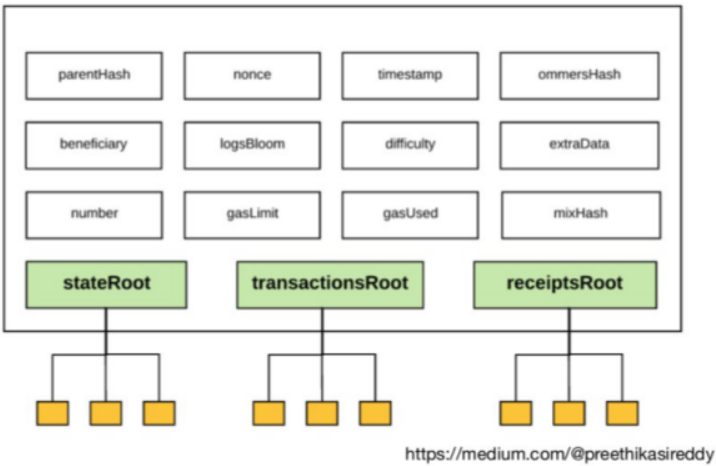
\includegraphics[width=0.7\textwidth]{./figs/eth-block.png}
		\caption{A structure of the header in Ethereum v1.0.}		
		\label{fig:eth-eth-header}
	\end{center}	
\end{figure}


\begin{itemize}
	\tightlist
	\item
	\textbf{Parent Hash}: The hash of the previous block's header, which
	links the blocks together in a chain.
	\item
	\textbf{Block Number}: The sequence number of the block in the chain.
	\item \textbf{Nonce}: replay protection counter.
	\item \textbf{Beneficiary}: the miner of the block -- replaces a coinbase transaction known from Bitcoin.
	\item
	\textbf{Timestamp}: The time at which the block was created.
	\item \textbf{ommersHash}: aggregates stale parent block headers whose miners get a certain partial reward.	
	\item
	\textbf{Difficulty}: The difficulty of the Proof-of-Work puzzle for
	the block.
	\item
	\textbf{Gas Limit and Gas Used}: The maximum amount of gas allowed in
	the block and the total amount of gas used by all the transactions in
	the block.
	\item
	\textbf{State Root, Transaction Root, and Receipt Root}: The root
	hashes of three Merkle-Patricia trees that store the global state, the
	transactions, and the transaction receipts, respectively.
	\item \textbf{ExtraData}: arbitrary data of max. 32B. (e.g., name of the mining pool)
	\item
	\textbf{Logs Bloom}: A Bloom filter that provides an efficient way to
	search for event logs generated by smart contracts within the block.
\end{itemize}

\subsubsection{The Global State and Merkle-Patricia
	Trees}\label{the-global-state-and-merkle-patricia-trees}

The \textbf{global state} of Ethereum is a massive data structure that
contains a mapping of all account addresses to their corresponding
account states. This state is not stored in the blockchain itself, but
rather in a separate key-value database that is maintained by all full
nodes.
The example of a transaction that calls smart contract account and thus changes the state is depicted in \autoref{fig:eth-state-change}.


\begin{figure}[t]
	%	\vspace{-0.3cm}
	\begin{center}
		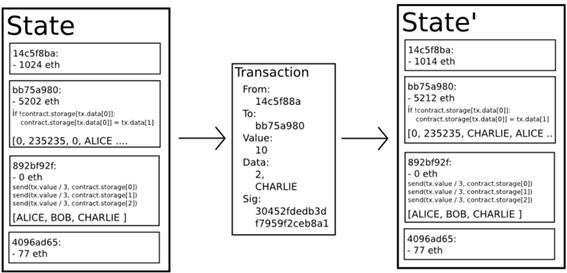
\includegraphics[width=0.7\textwidth]{./figs/eth-state-change.png}
		\caption{A transaction call that changes the state of the smart contract and its value.}		
		\label{fig:eth-state-change}
	\end{center}	
\end{figure}


To efficiently store and verify the global state, Ethereum uses a
sophisticated data structure called a \textbf{Merkle-Patricia Tree
	(MPT)}. The MPT is a hybrid data structure that combines the properties
of a Merkle tree (for integrity) and a Radix/Patricia trie (for
efficient lookups). This allows for efficient verification of the state
and enables light clients to securely query the state of an account
without having to download the entire blockchain. The root of the MPT,
known as the \textbf{state root}, is included in the block header, which
provides a cryptographic commitment to the entire state of the network
at that point in time.
MPT contains 3 types of nodes:
\begin{compactenum}
	\item \textbf{Extension nodes}: aggregate symbols in the key.
	\item \textbf{Branch nodes}: splits the path according to the current symbol in the key.
	\item \textbf{Leaf nodes}: they store data of the account states (or storages).	
\end{compactenum}
The example of ste state trie built using MPT is depicted in \autoref{fig:eth-mpt}, and it contains 4 accounts.

\begin{figure}[t]
	%	\vspace{-0.3cm}
	\begin{center}
		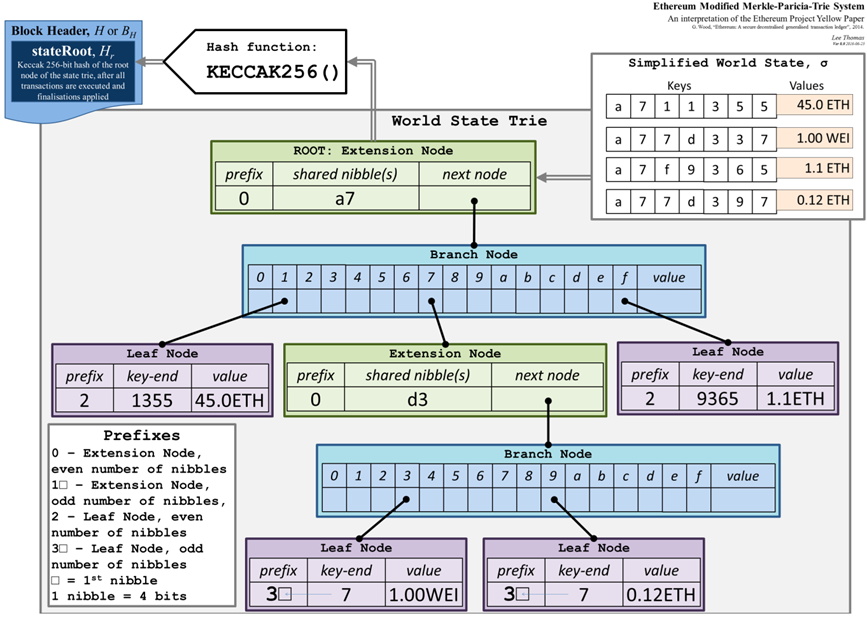
\includegraphics[width=0.95\textwidth]{./figs/eth-mpt.png}
		\caption{A Merkle-Patricia Trie for storing the global state in Ethereum.}		
		\label{fig:eth-mpt}
	\end{center}	
\end{figure}



\subsubsection{Bloom Filters and Transaction
	Receipts}\label{bloom-filters-and-transaction-receipts}

For every transaction, Ethereum generates a \textbf{receipt}, which
contains information about the outcome of the transaction, including the
gas used and, importantly, any \textbf{logs} or events emitted by the
smart contract during its execution.

To allow for efficient searching of these logs without requiring nodes
to scan every transaction in every block, Ethereum uses \textbf{Bloom
	filters}. A Bloom filter is a space-efficient probabilistic data
structure that can quickly test whether an element is a member of a set.
While it can produce false positives, it will never produce a false
negative.

Bloom filter is an $m$ bit array that requires $k$ different (cryptographically insecure) hash functions, where $k << m$. 
Bloom filter supports 2 operations:
\begin{compactenum}
	\item \textbf{Add element} -- we hash new element with k hash functions and set 1 on obtained positions.
	\item \textbf{Query element} -- we hash queried element with k hash functions and if 1 is on all positions, return true. Otherwise, return false (see \autoref{fig:eth-bloom-filter}).
\end{compactenum}
Bloom filter is often use as a pre-filter for expensive storage-lookup queries (see \autoref{fig:bloom-app}).

\begin{figure}[t]
	%	\vspace{-0.3cm}
	\begin{center}
		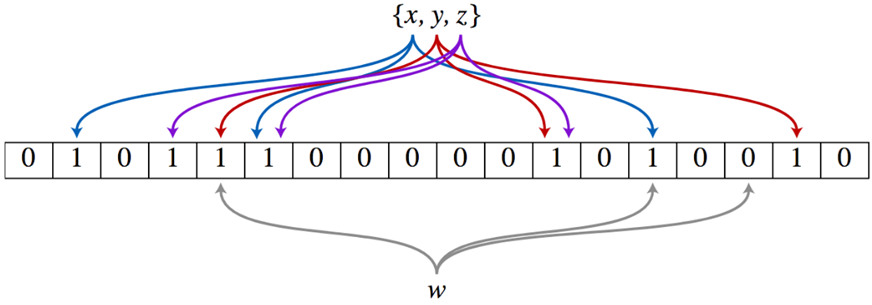
\includegraphics[width=0.9\textwidth]{./figs/bloom.png}
		\caption{An example of the Bloom filter with 3 hashing functions  and 3 elements. Element w in query is not included in the Bloom filter.}		
		\label{fig:eth-bloom-filter}
	\end{center}	
\end{figure}


\begin{figure}[t]
	%	\vspace{-0.3cm}
	\begin{center}
		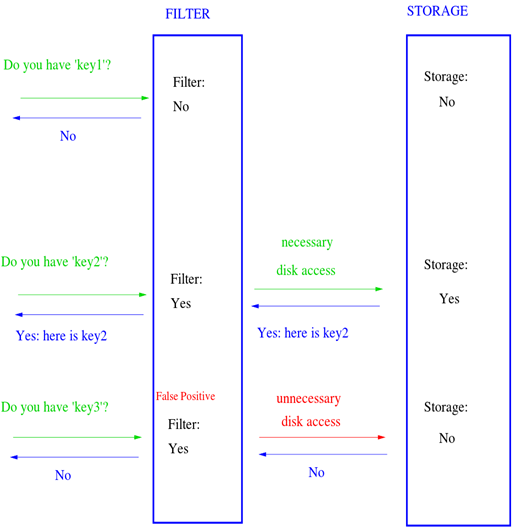
\includegraphics[width=0.7\textwidth]{./figs/bloom-eg.png}
		\caption{Application of Bloom filter for pre-filtering of queries.}		
		\label{fig:bloom-app}
	\end{center}	
\end{figure}



In Ethereum, each transaction receipt contains a Bloom filter of its logs, and the
block header contains a cumulative Bloom filter that aggregates the
filters from all transaction receipts in the block. This allows DAPPs
and light clients to quickly and efficiently find relevant events by
first checking the Bloom filter in the block header.




\begin{center}\rule{0.5\linewidth}{0.5pt}\end{center}

\subsection{Summary / Key Takeaways}\label{summary-key-takeaways}

This section has provided a comprehensive introduction to Ethereum, the
first and currently the most adopted platform for decentralized applications and smart
contracts. We have explored the historical context and motivation behind
its creation, highlighting the limitations of Bitcoin's scripting
language that spurred the development of a more general-purpose
blockchain.

We have delved into the core concepts that define the Ethereum
ecosystem, including:

\begin{itemize}
	\tightlist
	\item
	\textbf{Smart Contracts}: Self-executing contracts with the terms of
	the agreement directly written into code, enabling automation and
	reducing the need for intermediaries.
	\item
	\textbf{The Ethereum Virtual Machine (EVM)}: The sandboxed,
	deterministic runtime environment for smart contracts on the Ethereum
	network.
	\item
	\textbf{The Account-Based Model}: Ethereum's approach to tracking the
	state of the network, which is more intuitive for developers than
	Bitcoin's UTXO model.
	\item
	\textbf{Gas}: The mechanism for metering the computational resources
	of the network, preventing abuse and compensating miners.
	\item
	\textbf{Merkle-Patricia Trees}: The sophisticated data structure used
	to efficiently and securely store the global state of all accounts.
	\item
	\textbf{Bloom Filters}: A probabilistic data structure used to make
	searching for smart contract events highly efficient.
\end{itemize}


\begin{center}\rule{0.5\linewidth}{0.5pt}\end{center}

\subsection{Keywords}\label{keywords}

\begin{itemize}
	\tightlist
	\item
	\textbf{Ethereum}: A decentralized, open-source blockchain platform
	that enables the creation and deployment of smart contracts and
	decentralized applications (DAPPs).
	\item
	\textbf{Smart Contract}: A computer protocol intended to digitally
	facilitate, verify, or enforce the negotiation or performance of a
	contract.
	\item
	\textbf{Ethereum Virtual Machine (EVM)}: The runtime environment for
	smart contracts in Ethereum. It is a quasi-Turing-complete virtual
	machine that executes code as a sandboxed process.
	\item
	\textbf{Gas}: The unit of measurement for the computational effort
	required to execute operations on the Ethereum network.
	\item
	\textbf{Account Model}: An account model used in Ethereum where the
	state of the blockchain is represented as a set of accounts, each with
	its own balance, storage, and code.
	\item
	\textbf{Merkle-Patricia Tree (MPT)}: A hybrid data structure that
	combines a Merkle tree and a Patricia trie to efficiently store and
	verify the global state of the Ethereum network.
	\item
	\textbf{Externally Owned Account (EOA)}: An Ethereum account that is
	controlled by a user's private key.
	\item
	\textbf{Contract Account}: An Ethereum account that is controlled by
	the code of a smart contract.
	\item
	\textbf{Decentralized Finance (DeFi)}: A new financial system built on
	public blockchains that provides an alternative to traditional
	financial services.
	\item
	\textbf{Bloom Filter}: A space-efficient probabilistic data structure
	used in Ethereum to facilitate fast queries for log events.
\end{itemize}

\begin{center}\rule{0.5\linewidth}{0.5pt}\end{center}

\subsection{Further Reading}\label{further-reading}

\begin{itemize}
	\tightlist
	\item
	\textbf{Ethereum White Paper}: \\ 
	\url{https://ethereum.org/en/whitepaper/}
	\item
	\textbf{Ethereum Yellow Paper}: \\
	\url{https://ethereum.github.io/yellowpaper/paper.pdf}
	\item
	\textbf{Mastering Ethereum by Andreas M. Antonopoulos and Gavin Wood}: \\
	\url{https://github.com/ethereumbook/ethereumbook}
\end{itemize}

\newpage

\section{Smart Contract Programming}\label{chapter-6-smart-contract-programming}
This section provides a practical and in-depth introduction to the smart contract programming on the Ethereum blockchain.
Building upon the theoretical foundations laid in the previous section,
we will now transition to the practical aspects of designing,
developing, and deploying smart contracts. The primary focus of this
section will be on Solidity, the most widely adopted programming
language for writing smart contracts on the Ethereum platform.

We will begin by exploring the fundamental elements of the Solidity
language, including its syntax, data types, and control structures. We
will then move on to more advanced topics, such as the use of function
modifiers to create reusable code, the importance of visibility
specifiers for controlling access to functions and state variables, and
the use of libraries to promote code reuse and modularity.

A significant portion of this section will be dedicated to the practical
application of these concepts. We will examine the standards for
creating both fungible (ERC20) and non-fungible (ERC721) tokens, which
are two of the most common use cases for smart contracts on Ethereum.

Finally, we will address the critical topic of smart contract security.
We will discuss common vulnerabilities, such as reentrancy attacks and
integer overflows, and we will explore the best practices and tools that
developers can use to write secure and robust smart contracts. By the
end of this section, you will have the foundational knowledge and
practical skills necessary to begin your journey as a smart contract
developer.

\subsection{Learning Objectives}\label{learning-objectives}

\begin{itemize}
	\tightlist
	\item
	Understand the basics of the Solidity programming language.
	\item
	Learn how to define and interact with smart contracts.
	\item
	Grasp the concepts of visibility specifiers, function modifiers, and
	data locations.
	\item
	Understand the role of fallback and receive functions in handling
	Ether transfers.
	\item
	Learn about the standards for fungible (ERC20) and non-fungible
	(ERC721) tokens.
	\item
	Gain insight into common smart contract vulnerabilities and security
	best practices.
	\item
	Become familiar with the tools and techniques used for smart contract
	development and analysis.
\end{itemize}

\begin{center}\rule{0.5\linewidth}{0.5pt}\end{center}

\subsection{Introduction to
	Solidity}\label{section-1-introduction-to-solidity}

\subsubsection{What is Solidity?}\label{what-is-solidity}

Solidity is a high-level, object-oriented programming language that has
become the de facto standard for writing smart contracts on the Ethereum
blockchain and other EVM-compatible platforms. It is a statically-typed
language with a syntax that is similar to that of JavaScript and C++,
making it relatively easy for developers with experience in these
languages to learn.

The primary purpose of Solidity is to provide a means for developers to
create self-executing contracts that can be deployed to a blockchain.
These contracts can be used to automate a wide range of processes, from
simple token transfers to complex financial instruments.
The users interact with smart contracts through decentralized applications (DAPPs), which run completely server-less -- on the client side (see \autoref{fig:dapps}).


\begin{figure}[t]
	%	\vspace{-0.3cm}
	\begin{center}
		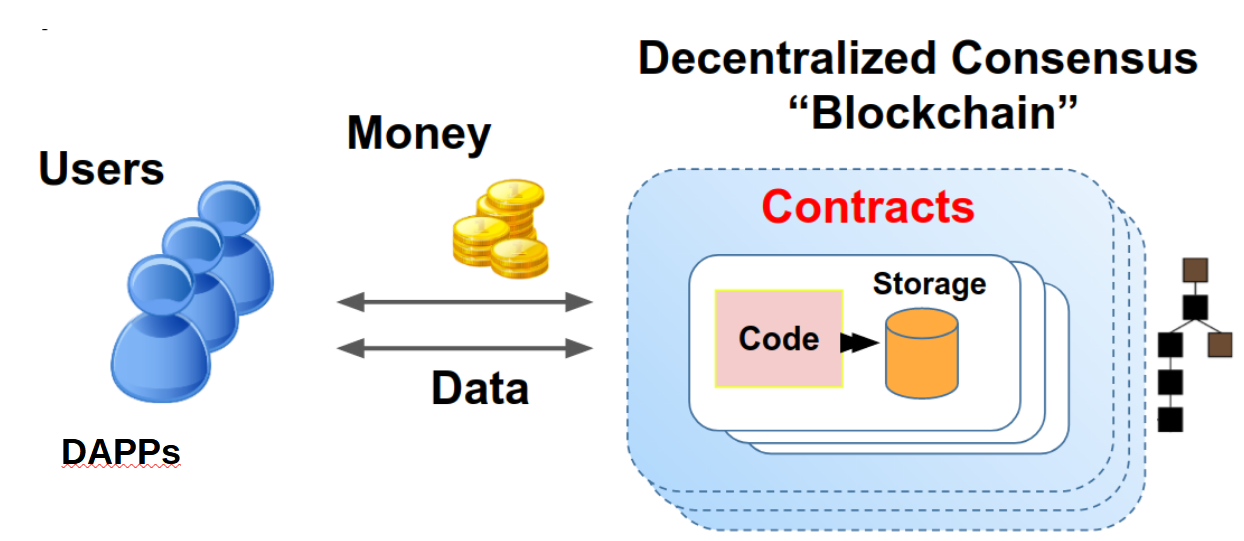
\includegraphics[width=0.8\textwidth]{./figs/smart-contracts-flow.png}
		\caption{Users interacting with smart contract through DAPPs (that run on the client-side).}		
		\label{fig:dapps}
	\end{center}	
\end{figure}
  

\subsubsection{The Structure of a Solidity
	Contract}\label{the-structure-of-a-solidity-contract}

A Solidity contract is a collection of code and data that is deployed to
a specific address on the blockchain. It is analogous to a class in an
object-oriented programming language, in that it encapsulates both data
(in the form of state variables) and behavior (in the form of
functions).

A typical Solidity source file has the following structure:

\begin{itemize}
	\tightlist
	\item
	\textbf{Pragma Directive}: This is a declaration that specifies the
	version of the Solidity compiler that should be used to compile the
	code. This is important for ensuring that the code is compiled
	correctly and that it is compatible with the target version of the
	EVM.
	\item
	\textbf{License Identifier}: This is a comment that specifies the
	license under which the code is released. This is important for legal
	and ethical reasons, as it informs other developers of the terms under
	which they can use and modify the code.
	\item
	\textbf{Contract Definition}: This is the main body of the contract,
	which contains the state variables, functions, events, and modifiers
	that define the contract's behavior.
\end{itemize}
See an example of a smart contract in \autoref{fig:smart-contract}.


\begin{figure}[t]
	%	\vspace{-0.3cm}
	\begin{center}
		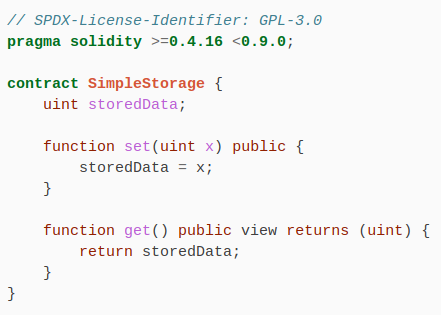
\includegraphics[width=0.5\textwidth]{./figs/smart-contract-example.png}
		\caption{Example of simple smart contract written in Solidity.}		
		\label{fig:smart-contract}
	\end{center}	
\end{figure}


\subsubsection{Data Types and
	Variables}\label{data-types-and-variables}

Solidity supports a rich set of data types, which can be broadly
classified into two categories:

\begin{itemize}
	\tightlist
	\item
	\textbf{Value Types}: These are data types that are passed by value,
	meaning that a copy of the value is created when it is assigned to a
	new variable or passed as an argument to a function. Value types
	include \texttt{bool}, \texttt{int}, \texttt{uint}, \texttt{address},
	and \texttt{bytes}.
	\item
	\textbf{Reference Types}: These are data types that are passed by
	reference, meaning that the new variable or function argument refers
	to the same location in memory as the original. Reference types
	include \texttt{arrays}, \texttt{structs}, and \texttt{mappings}.
\end{itemize}

Variables in Solidity can be stored in one of three data locations:

\begin{itemize}
	\tightlist
	\item
	\textbf{Storage}: This is the persistent storage of the contract,
	which is stored on the blockchain. State variables are stored in
	storage by default. It is the most expensive place in terms of gas since it is permanent.
	\item
	\textbf{Memory}: This is a temporary storage location that is cleared
	between function calls. It is used to store local variables and
	function arguments. In general, the memory is not permanent storage and thus operations with memory are cheap in terms of gas.
	\item
	\textbf{Calldata}: This is a read-only storage location that is used
	to store the input data for a function call. In fact, calldata location is also stored in memory and thus has the same cost implications in terms of gas.
\end{itemize}

\begin{center}\rule{0.5\linewidth}{0.5pt}\end{center}

\subsection{Functions and Control
	Structures}\label{section-2-functions-and-control-structures}

\subsubsection{Functions}\label{functions}

Functions are the fundamental units of execution in a Solidity smart
contract. They encapsulate the logic of the contract and can be called
either internally by other functions within the same contract or
externally by other contracts or users.

Solidity provides four visibility specifiers for functions, which
control how they can be accessed:

\begin{itemize}
	\tightlist
	\item
	\textbf{\texttt{public}}: Public functions can be called from
	anywhere, both internally and externally.
	\item
	\textbf{\texttt{private}}: Private functions can only be called from
	within the contract in which they are defined.
	\item
	\textbf{\texttt{internal}}: Internal functions can be called from
	within the contract in which they are defined and from any contracts
	that inherit from it.
	\item
	\textbf{\texttt{external}}: External functions can only be called from
	outside the contract.
\end{itemize}

In addition to visibility specifiers, functions can also have modifiers
that alter their behavior. The most common modifiers are:

\begin{itemize}
	\tightlist
	\item
	\textbf{\texttt{view}}: This modifier indicates that the function is
	read-only and does not modify the state of the contract.
	\item
	\textbf{\texttt{pure}}: This modifier indicates that the function does
	not read or modify the state of the contract.
	\item
	\textbf{\texttt{payable}}: This modifier indicates that the function
	can receive Ether.
\end{itemize}

Note that Solidity provides several globally available variables and functions that are specific either to the current transaction or the block in which the transaction is included. 
The most important such functions and variables are presented in \autoref{fig:special-vars} and \autoref{fig:special-vars2}.

\begin{figure}[t]
	%	\vspace{-0.3cm}
	\begin{center}
		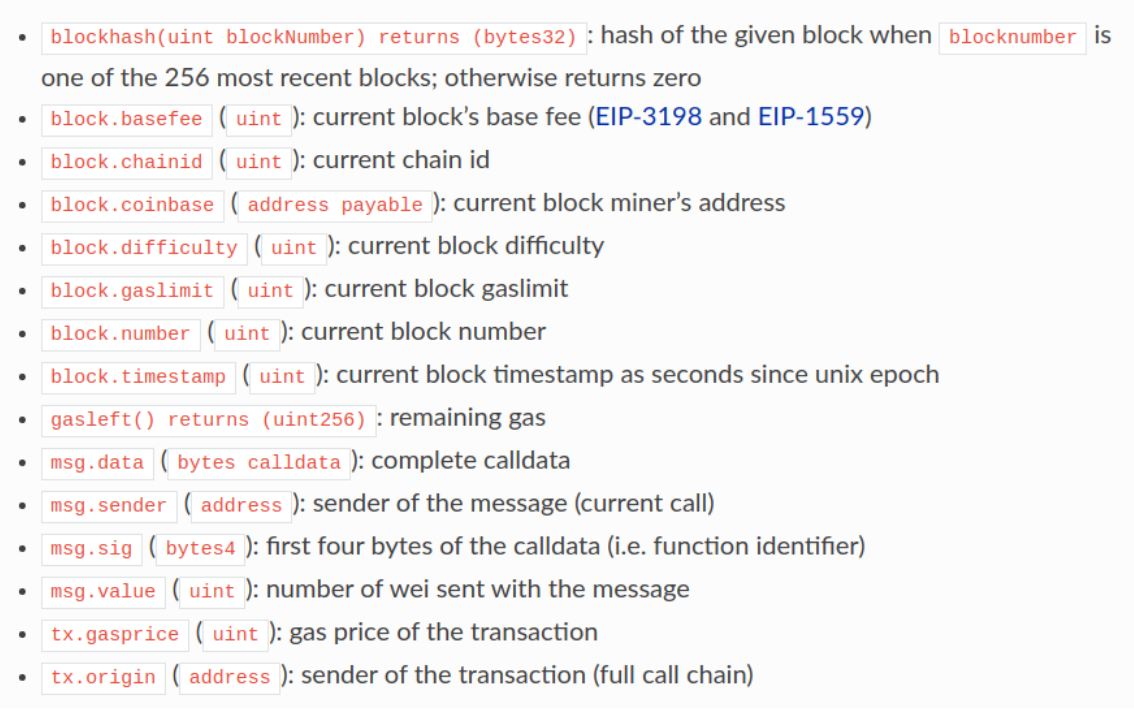
\includegraphics[width=0.9\textwidth]{./figs/vars-funcs.png}
		\caption{Globally available variables and functions.}		
		\label{fig:special-vars}
	\end{center}	
\end{figure}

\begin{figure}[t]
	%	\vspace{-0.3cm}
	\begin{center}
		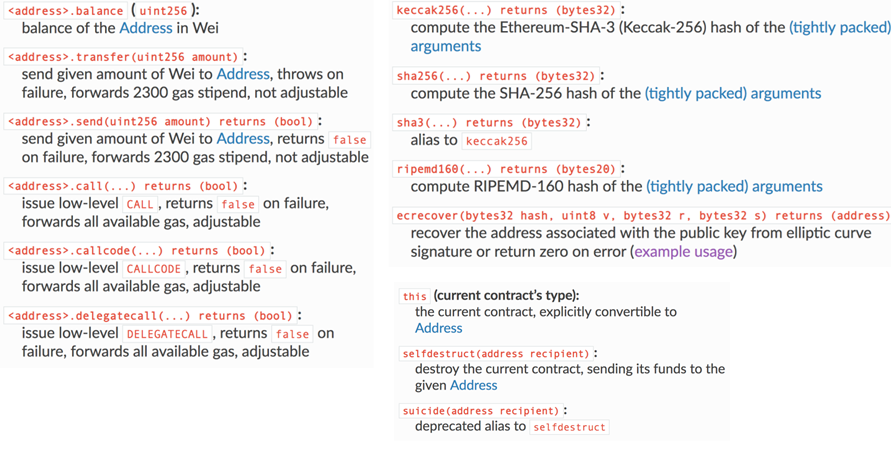
\includegraphics[width=0.99\textwidth]{./figs/functions2.png}
		\caption{Globally available variables and functions.}		
		\label{fig:special-vars2}
	\end{center}	
\end{figure}

\subsubsection{Control Structures}\label{control-structures}

Solidity supports a range of standard control structures that are common
to many programming languages, including:

\begin{itemize}
	\tightlist
	\item
	\textbf{Conditional statements}: \texttt{if}, \texttt{else}
	\item
	\textbf{Loops}: \texttt{while}, \texttt{for}, \texttt{do-while}
\end{itemize}

Solidity also provides three error-handling mechanisms that can be used
to revert the state of the contract if an error occurs:

\begin{itemize}
	\tightlist
	\item
	\textbf{\texttt{require}}: This function is used to validate inputs
	and conditions before executing a function. If the condition is not
	met, the transaction is reverted.
	\item
	\textbf{\texttt{assert}}: This function is used to check for internal
	errors and to validate invariants. If the condition is not met, the
	transaction is reverted.
	\item
	\textbf{\texttt{revert}}: This function is used to revert the
	transaction and provide an error message.
\end{itemize}

\subsubsection{\texorpdfstring{Special Functions: \texttt{receive}
		and
		\texttt{fallback}}{Special Functions: receive and fallback}}\label{special-functions-receive-and-fallback}

Solidity includes two special functions that are used to handle Ether
transfers and calls to non-existent functions:

\begin{itemize}
	\tightlist
	\item
	\textbf{\texttt{receive} function}: This function is executed when a
	contract receives a plain Ether transfer without any accompanying
	data. It must be declared as \texttt{external} and \texttt{payable}.
	\item
	\textbf{\texttt{fallback} function}: This function is executed when a
	contract receives a call to a function that does not exist in the
	contract. It can also be used to receive Ether if no \texttt{receive}
	function is defined.
\end{itemize}

These functions are essential for creating contracts that can interact
with the Ethereum network in a flexible and robust manner.


\subsubsection{Custom function modifiers}\label{sec:modifiers}
Solidity provides custom modifiers of functions that act in a similar fashion as macros in C/C++.
These custom modifiers are usually used to check authorization for calling the function or conditions to be met.
See two examples of custom function modifiers in \autoref{fig:modifiers}.

\begin{figure}[t]
	%	\vspace{-0.3cm}
	\begin{center}
		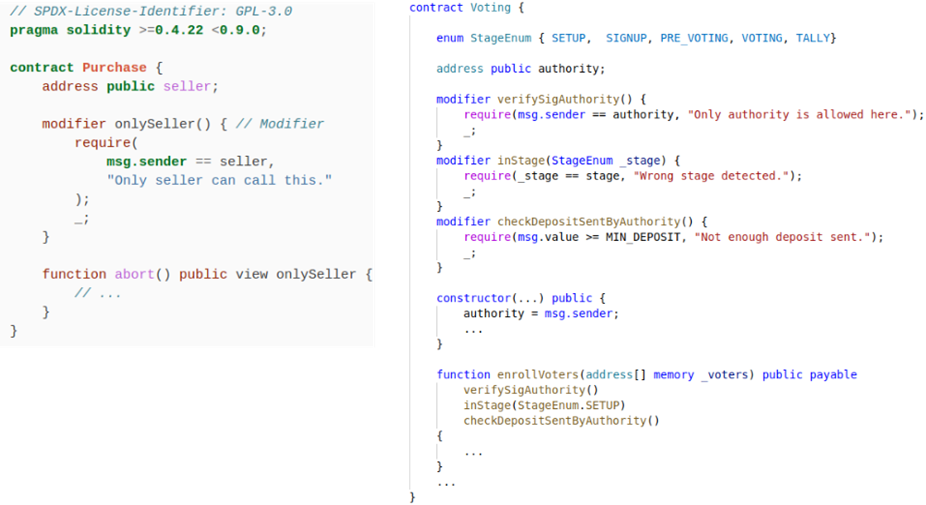
\includegraphics[width=0.9\textwidth]{./figs/modifiers-custom.png}
		\caption{Examples of custom function modifiers.}		
		\label{fig:modifiers}
	\end{center}	
\end{figure}

\subsubsection{Abstract contracts and interfaces}\label{sec:interfaces}
Similarly to  many other object-oriented programming languages, Solidity also supports abstract contracts and interfaces.
Contract is marked as abstract if at least one of its functions is not implemented. In contrast, interfaces must have not any function implemented.
See examples of abstract contract and interface in \autoref{fig:inteface}. 

\begin{figure}[bt]
	%	\vspace{-0.3cm}
	\begin{center}
		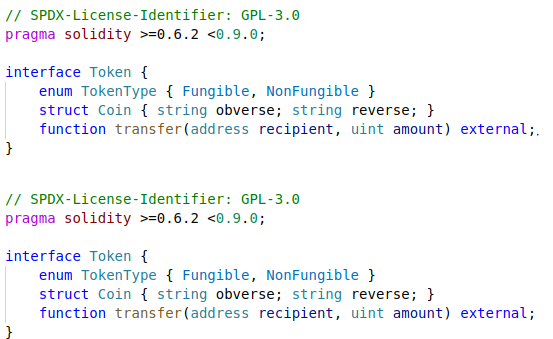
\includegraphics[width=0.7\textwidth]{./figs/abstract-contract.png }
		\caption{Examples of abstract contract and interface.}		
		\label{fig:inteface}
	\end{center}	
\end{figure}



\subsubsection{Libraries}\label{sec:libs}
Libraries are similar to contracts but they are deployed only once and their code is reused using the DELEGATECALL instruction.
If library functions are called, their code is executed in the context of the calling contract (especially modifying the storage of the calling contract).
Therefore, libraries are assumed to be stateless.
Libraries can be also seen as implicit base contracts of the contracts that use them.
An example of the library and its application to a specific data type is depicted in \autoref{fig:library}. 
Another example of library is depicted in \autoref{fig:library2}.


\begin{figure}[bt]
	%	\vspace{-0.3cm}
	\begin{center}
		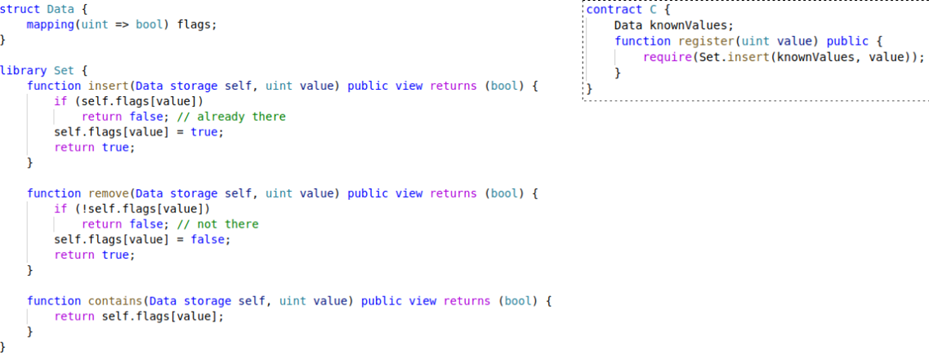
\includegraphics[width=0.99\textwidth]{./figs/library.png }
		\caption{The example of library contract and its application on a data type.}		
		\label{fig:library}
	\end{center}	
\end{figure}

\begin{figure}[bt]
	%	\vspace{-0.3cm}
	\begin{center}
		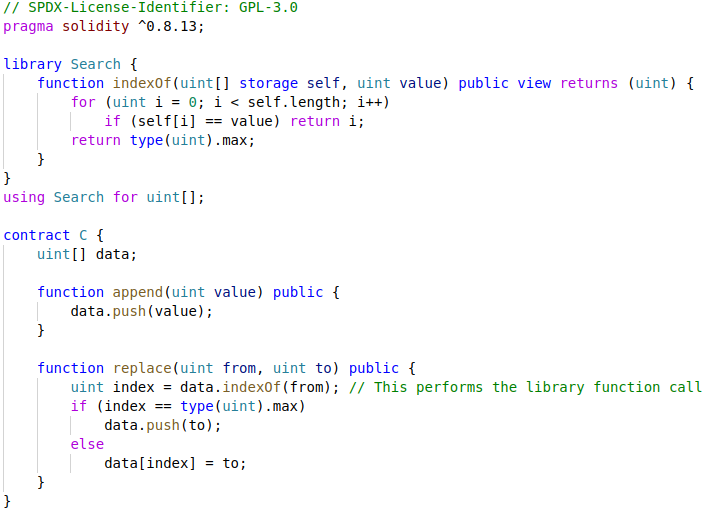
\includegraphics[width=0.8\textwidth]{./figs/library2.png }
		\caption{The example of library contract and its application using ``using'' and ``for''.}		
		\label{fig:library2}
	\end{center}	
\end{figure}



\begin{center}\rule{0.5\linewidth}{0.5pt}\end{center}

\subsection{Token Standards and Smart Contract
	Security}\label{section-3-token-standards-and-smart-contract-security}

\subsubsection{ERC20 and ERC721 Token
	Standards}\label{erc20-and-erc721-token-standards}

To promote interoperability and composability within the Ethereum
ecosystem, the community has developed a set of standards for different
types of tokens. The two most widely adopted standards are ERC20 and
ERC721.

\begin{itemize}
	\tightlist
	\item
	\textbf{ERC20}: This is the standard for fungible tokens, which are
	tokens that are identical and interchangeable. Examples of ERC20
	tokens include stablecoins like USDT and DAI, as well as governance
	tokens for various DeFi protocols. The ERC20 standard defines a common
	interface that includes functions for transferring tokens, checking
	account balances, and approving other accounts to spend tokens on
	behalf of the owner.
	The interface of ERC20 contract is depicted in \autoref{fig:erc20}.
\end{itemize}

\begin{figure}[t]
	%	\vspace{-0.3cm}
	\begin{center}
		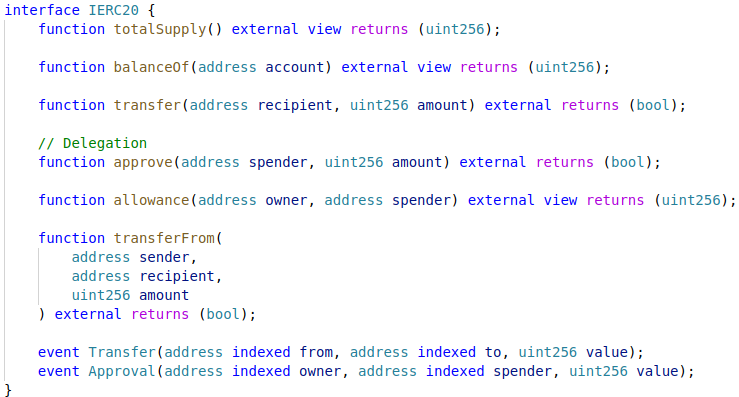
\includegraphics[width=0.9\textwidth]{./figs/ERC20.png }
		\caption{ERC20 interface.}		
		\label{fig:erc20}
	\end{center}	
\end{figure}
\begin{figure}
	%	\vspace{-0.3cm}
	\begin{center}
		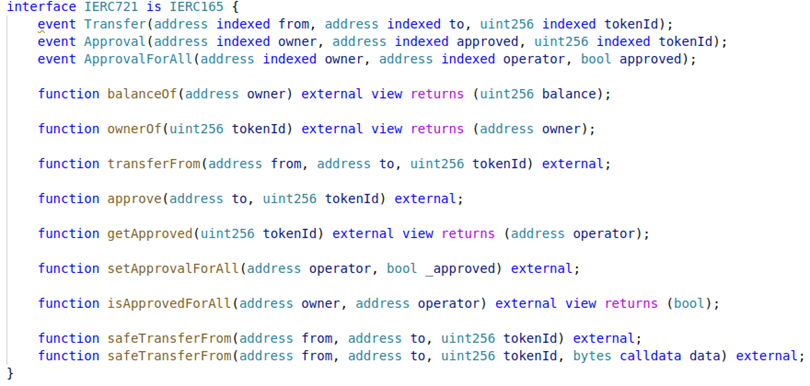
\includegraphics[width=0.9\textwidth]{./figs/ERC721.png }
		\caption{ERC721 interface.}		
		\label{fig:erc721}
	\end{center}	
\end{figure}


\begin{itemize}
	\tightlist
	\item
	\textbf{ERC721}: This is the standard for non-fungible tokens (NFTs),
	which are unique and non-interchangeable. Each ERC721 token has a
	unique ID and can be used to represent a wide range of assets, from
	digital art and collectibles to real estate and intellectual property.
	The ERC721 standard defines a common interface for tracking the
	ownership of each individual token.
	The interface of ERC721 contract is depicted in \autoref{fig:erc721}.
\end{itemize}




These token standards have been instrumental in the growth of the
Ethereum ecosystem, as they allow for seamless integration between
different applications, such as wallets, exchanges, and DeFi protocols.




\clearpage
\subsubsection{Smart Contract
	Security}\label{smart-contract-security}

The immutable nature of blockchains means that bugs and vulnerabilities
in smart contracts can have severe and irreversible consequences, often
leading to significant financial losses. Therefore, smart contract
security is of paramount importance. Some of the most common security
vulnerabilities include:

\begin{itemize}
	\tightlist
	\item
	\textbf{Reentrancy Attacks}: This is a type of attack where a
	malicious contract can repeatedly call a function on a victim contract
	before the first call has completed. This can be used to drain funds
	from the victim contract if it does not follow the
	checks-effects-interactions pattern. The infamous DAO attack was a
	result of a reentrancy vulnerability (see \autoref{fig:dao-bug}).
\end{itemize}


\begin{figure}[t]
	%	\vspace{-0.3cm}
	\begin{center}
		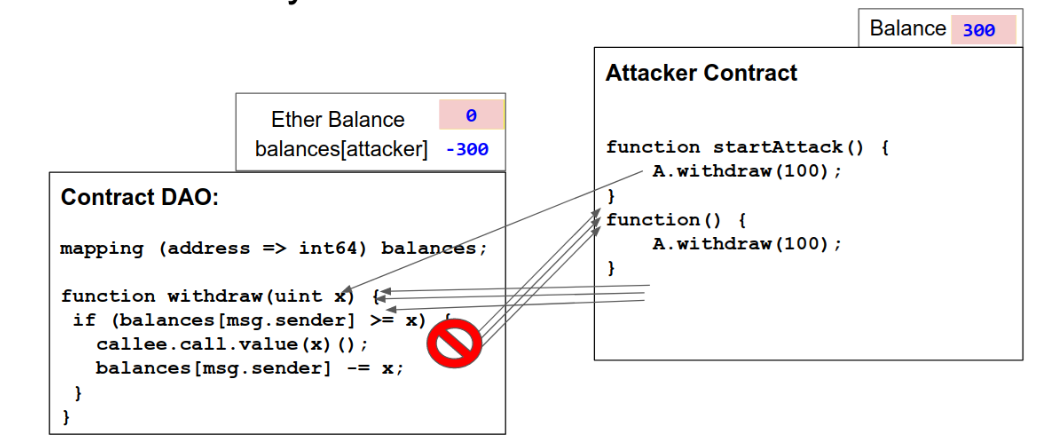
\includegraphics[width=0.9\textwidth]{./figs/DAO.png }
		\caption{Reentrancy vulnerability in DAO bug.}		
		\label{fig:dao-bug}
	\end{center}	
\end{figure}

\begin{itemize}
	\tightlist
	\item
	\textbf{Integer Overflows and Underflows}: These vulnerabilities occur
	when an arithmetic operation results in a value that is outside the
	range of the data type. This can lead to unexpected behavior and can
	be exploited by attackers to manipulate the state of the contract.
	It can, for example, cause out of gas exception due to comparing mismatching data types:  \verb| for (var i = 0; i < 2000; i++) { ... } |. Note that i is of type uint8 and thus will never reach the value 2000.
	
%	\begin{figure}[t]
%		%	\vspace{-0.3cm}
%		\begin{center}
%			\includegraphics[width=0.8\textwidth]{./figs/underflow.png }
%			\caption{Out of gas exception due to integer underflow.}		
%			\label{fig:underflow}
%		\end{center}	
%	\end{figure}
	
	\item
	\textbf{Denial-of-Service (DoS) Attacks}: An attacker can exploit
	certain vulnerabilities to render a contract unusable, for example, by
	causing it to run out of gas or by making it impossible for other
	users to interact with it.
\end{itemize}

Another notable example of smart contract vulnerabilities is the Parity
Wallet bug, which led to the freezing of millions of dollars worth of
Ether. This bug was caused by a flaw in the way the wallet's library
contract was initialized, allowing an attacker to take ownership of the
library and self-destruct it.

\subsubsection{Upgradeable Smart
	Contracts}\label{upgradeable-smart-contracts}

While smart contracts are immutable by default, there are scenarios
where it is desirable to be able to modify them, for example, to fix a
bug or to add new functionality. The Proxy and Implementation pattern is
a common approach to creating upgradeable smart contracts. This pattern
involves a proxy contract that stores the state of the contract and
delegates all calls to an implementation contract (see \autoref{fig:upgradable}). The implementation
contract can be replaced with a new version without affecting the state
of the proxy contract.

\begin{figure}[t]
	%	\vspace{-0.3cm}
	\begin{center}
		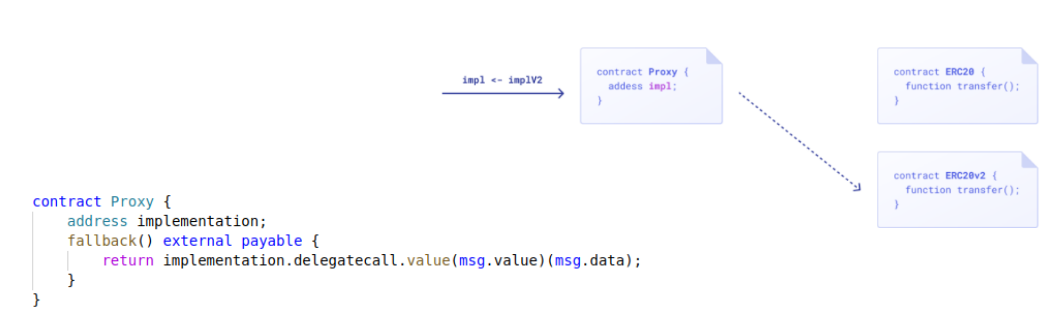
\includegraphics[width=0.99\textwidth]{./figs/upgradable.png}
		\caption{Proxy and implementation pattern.}		
		\label{fig:upgradable}
	\end{center}	
\end{figure}


\subsubsection{Tools for Smart Contract Development and
	Analysis}\label{tools-for-smart-contract-development-and-analysis}

A rich ecosystem of tools has emerged to support the development and
analysis of secure and robust smart contracts. These tools can be
broadly categorized as follows:

\begin{itemize}
	\tightlist
	\item
	\textbf{Development Frameworks}: These provide a comprehensive
	environment for compiling, testing, and deploying smart contracts.
	Popular frameworks include Truffle and Hardhat.
	\item
	\textbf{Browser-Based IDEs}: These provide a convenient and
	user-friendly environment for writing and testing smart contracts
	directly in the browser. Remix is the most widely used browser-based
	IDE.
	\item
	\textbf{Static Analysis Tools}: These tools analyze the source code of
	a smart contract to identify potential vulnerabilities and deviations
	from best practices. Examples include Slither and Solhint.
	\item
	\textbf{Dynamic Analysis Tools}: These tools analyze the behavior of a
	smart contract as it is being executed to identify vulnerabilities
	that may not be apparent from a static analysis. Examples include
	Echidna and Manticore.
\end{itemize}

\begin{center}\rule{0.5\linewidth}{0.5pt}\end{center}

\subsection{Summary / Key Takeaways}\label{summary-key-takeaways}

This section has provided a practical, hands-on introduction to the
world of smart contract programming with Solidity. We have covered the
essential elements of the language, from its basic syntax and data types
to its more advanced features, such as function modifiers and visibility
specifiers.

We have explored the structure of a Solidity contract and the different
data locations that can be used to store variables. We have also
examined the role of special functions like \texttt{receive} and
\texttt{fallback} in handling Ether transfers and interacting with other
contracts.

A key focus of this section has been on the practical application of
Solidity. We have discussed the ERC20 and ERC721 token standards, which
are the foundation of the vibrant DeFi and NFT ecosystems on Ethereum.

Finally, we have addressed the critical importance of smart contract
security. We have identified common vulnerabilities, such as reentrancy
attacks and integer overflows, and we have highlighted the tools and
best practices that developers can use to write secure and robust code.

By the end of this section, you should have a solid foundation in smart
contract programming and be well-equipped to start building your own
decentralized applications on the Ethereum blockchain.

\begin{center}\rule{0.5\linewidth}{0.5pt}\end{center}

\subsection{Keywords}\label{keywords}

\begin{itemize}
	\tightlist
	\item
	\textbf{Solidity}: A high-level, object-oriented programming language
	for writing smart contracts on the Ethereum blockchain.
	\item
	\textbf{Smart Contract}: A self-executing contract with the terms of
	the agreement between buyer and seller being directly written into
	lines of code.
	\item
	\textbf{ERC20}: A technical standard used for smart contracts on the
	Ethereum blockchain for implementing tokens.
	\item
	\textbf{ERC721}: A standard for non-fungible tokens (NFTs) on the
	Ethereum blockchain.
	\item
	\textbf{Reentrancy}: A common smart contract vulnerability where a
	malicious contract can repeatedly call a function on a victim contract
	before the first call has completed.
	\item
	\textbf{Visibility Specifiers}: Keywords in Solidity that control the
	accessibility of functions and state variables.
	\item
	\textbf{Function Modifiers}: Reusable pieces of code that can be used
	to change the behavior of functions in a declarative way.
	\item
	\textbf{Truffle}: A popular development framework for Ethereum that
	provides a suite of tools for compiling, testing, and deploying smart
	contracts.
	\item
	\textbf{Hardhat}: A flexible and extensible Ethereum development
	environment that is widely used for smart contract development.
	\item
	\textbf{Remix}: A browser-based IDE for Solidity that provides a
	convenient environment for writing, testing, and deploying smart
	contracts.
\end{itemize}

\begin{center}\rule{0.5\linewidth}{0.5pt}\end{center}

\subsection{Further Reading}\label{further-reading}

\begin{itemize}
	\tightlist
	\item
	\textbf{Solidity Documentation}: \\
	\url{https://docs.soliditylang.org/}
	\item
	\textbf{OpenZeppelin Contracts}: \\
	\url{https://github.com/OpenZeppelin/openzeppelin-contracts}
	\item
	\textbf{ConsenSys Smart Contract Best Practices}: \\
	\url{https://consensys.github.io/smart-contract-best-practices/}
\end{itemize}



%\chapter{tmp}\label{chapter:intro}
%BLA BLA~\cite{homoliak2019security}




%%%%%%%%%%%%%%%%%%%%%%%%%%%%%%%%%%%%%%%%%%%%%%%%%%%%%%%%%%%%%%%%%%%%%%%%%%%%%%%
\clearpage

\addcontentsline{toc}{chapter}{\\Bibliography}
\bibliographystyle{alpha}
\bibliography{./refs/ref,./refs/ref2,./refs/ref3,./refs/ref4,./refs/ref5,./refs/ref6,./refs/ref7,./refs/ref8,./refs/ref9}
%%%%%%%%%%%%%%%%%%%%%%%%%%%%%%%%%%%%%%%%%%%%%%%%%%%%%%%%%%%%%%%%%%%%%%%%%%%%%%%



\pagenumbering{gobble}


%%%%%%%%%%%%%%%%%%%%%%%%%%%%%%%%%%%%%%%%%%%%%%%%%%%%%%%%%%%%%%%%%%%%%%%%%%%%%%%
\end{document} 
%%%%%%%%%%%%%%%%%%%%%%%%%%%%%%%%%%%%%%%%%%%%%%%%%%%%%%%%%%%%%%%%%%%%%%%%%%%%%%%
